\documentclass[11pt,letterpaper]{article}
\usepackage[margin=0.95in,top=0.95in,bottom=0.95in]{geometry}
\usepackage{fontspec}
\usepackage{xeCJK}
\usepackage{amsmath,amssymb}
\usepackage{booktabs,array,adjustbox,makecell,longtable}
\usepackage[table]{xcolor}
\usepackage{graphicx}
\usepackage{caption}
\usepackage{fancyhdr}
\usepackage{enumitem}
\usepackage[most]{tcolorbox}
\usepackage[hidelinks,bookmarks=true,bookmarksnumbered=false]{hyperref}
\usepackage{titlesec}
\usepackage{needspace}

\setmainfont{Palatino}
\setmonofont[Scale=0.82]{Menlo}
\setCJKmainfont[AutoFakeBold=2.0,ItalicFont={Kaiti SC}]{Songti SC}
\setCJKsansfont{PingFang SC}
\setCJKmonofont{PingFang SC}
\xeCJKsetup{CJKecglue=\hspace{0.12em plus 0.04em minus 0.02em}}
\linespread{1.22}
\setlength{\heavyrulewidth}{0.09em}
\setlength{\lightrulewidth}{0.05em}
\setlength{\cmidrulewidth}{0.04em}

\definecolor{NavyAccent}{HTML}{111827}
\definecolor{CrimsonAccent}{HTML}{9B2C2C}
\definecolor{PanelTint}{HTML}{F8FAFC}
\definecolor{RuleGray}{HTML}{CBD5E1}
\definecolor{MutedText}{HTML}{374151}

\captionsetup[table]{
  font={small,bf},
  labelfont={bf},
  justification=raggedright,
  singlelinecheck=false,
  skip=4pt
}
\captionsetup[figure]{
  font={small},
  labelfont={bf},
  justification=centering,
  skip=6pt
}

\titleformat{\section}[block]{\large\bfseries\color{NavyAccent}}{}{0pt}{}
\titlespacing*{\section}{0pt}{15pt}{5pt}
\titleformat{\subsection}[block]{\normalsize\bfseries\itshape\color{NavyAccent}}{}{0pt}{}
\titlespacing*{\subsection}{0pt}{11pt}{4pt}
\titleformat{\subsubsection}[block]{\normalsize\itshape\color{MutedText}}{}{0pt}{}
\titlespacing*{\subsubsection}{0pt}{8pt}{3pt}

\setlist[itemize]{leftmargin=1.5em,itemsep=2pt,topsep=4pt,parsep=1pt}
\setlist[enumerate]{leftmargin=1.7em,itemsep=2pt,topsep=4pt,parsep=1pt}
\setlength{\parindent}{0pt}
\setlength{\parskip}{6pt}
\setlength{\emergencystretch}{3em}
\sloppy

\newtcolorbox{calloutbox}[2]{
  enhanced,
  breakable,
  colback={#1!5!white},
  colframe={#1},
  boxrule=0pt,
  leftrule=3pt,
  arc=2pt,
  left=8pt,
  right=8pt,
  top=6pt,
  bottom=6pt,
  fonttitle=\small\bfseries,
  coltitle={#1},
  colbacktitle={#1!5!white},
  title={#2}
}

\pagestyle{fancy}
\fancyhf{}
\fancyhead[L]{\scriptsize\color{MutedText} Hong Kong’s IPO Market: A Financial History, 1891–2026}
\fancyhead[R]{\scriptsize\color{MutedText} \rightmark}
\fancyfoot[C]{\small\color{MutedText} \thepage}
\renewcommand{\headrulewidth}{0.3pt}
\renewcommand{\footrulewidth}{0pt}

\begin{document}
\thispagestyle{plain}

\begin{center}
{\LARGE\bfseries Hong Kong’s IPO Market: A Financial History of the City, China, and Global Capital, 1891–2026 \par}
\vspace{10pt}
{\normalsize \textit{Comprehensive Research Monograph — Historical Coverage: 1891–2026; Reconciled IPO Census: January 1994–September 2026; Market Observation Cutoff: November 12, 2026} \par}
\vspace{10pt}
\end{center}

\begin{quote}
\small
\begin{center}\textbf{Abstract}\end{center}
\vspace{-4pt}
\noindent Mainland Chinese companies needed equity capital, and international investors needed confidence that they could enforce their shareholder rights and repatriate their proceeds. Hong Kong connected the two sides through a convertible currency, enforceable shareholder protections, and intermediaries accountable for disclosure. We examine this cross-border bridge across 135 years of market history (1891–2026) and a reconciled census of all 2,866 ordinary operating-company initial public offerings (HK\$5.66 trillion in gross proceeds) completed between January 1994 and September 2026. Our empirical question is how the terms of an offering, namely the entry price, the allocation rules, and the cost of financing an application, change what investors actually receive; the institutional history explains why those terms took the form they did. Investor outcomes were strikingly uneven: by November 2026, roughly three-quarters (77.5\%) of the 2,117 verified IPOs traded below their offer price, yet the shares sold at IPO recorded HK\$3.71 trillion in cumulative net price gains before dividends because just 21 companies, led by Tencent and AIA, generated nearly three-quarters (73.8\%) of gross gains among appreciating offerings. Entry price matters as much as the issuer: the same one-year holding beats an estimated dividend-reinvested Hang Seng benchmark when bought at the offer price and trails it when bought at the first-day close. Ballot schedules show that a 53\% average first-day return from the offer price in 2026 shrank to about 2\% per dollar applied for on a one-lot cash application and to roughly zero on a large financed application. Issuers also paid fixed verification costs that weighed most on small offerings, and the city built a recurring business in trading, clearing, and professional services that exceeds listing fees.
\par\smallskip\noindent \textbf{JEL Classification:} G15, G18, G24, G32, K22, N25
\par\smallskip\noindent \textbf{Keywords:} Hong Kong IPOs, Cross-Border Capital Formation, Trust Production, Institutional Bonding, Cornerstone Investors, Long-Run Return Skewness
\end{quote}
\vspace{8pt}
\noindent\rule{\linewidth}{0.4pt}
\vspace{6pt}

\clearpage
\begingroup
\small
\setlength{\parskip}{2pt}
\setcounter{tocdepth}{2}
\renewcommand{\contentsname}{Contents}
\tableofcontents
\endgroup
\clearpage


\section*{\texorpdfstring{Section 1. Introduction: Capital Formation, Institutional Bridges, and Distributional Trade-offs}{Section 1. Introduction: Capital Formation, Institutional Bridges, and Distributional Trade-offs}}
\addcontentsline{toc}{section}{\texorpdfstring{Section 1. Introduction: Capital Formation, Institutional Bridges, and Distributional Trade-offs}{Section 1. Introduction: Capital Formation, Institutional Bridges, and Distributional Trade-offs}}
\markright{Section 1. Introduction}
\subsection*{\texorpdfstring{1.1 The Cross-Border Financing Problem, Research Question, and Main Findings}{1.1 The Cross-Border Financing Problem, Research Question, and Main Findings}}
\addcontentsline{toc}{subsection}{\texorpdfstring{1.1 The Cross-Border Financing Problem, Research Question, and Main Findings}{1.1 The Cross-Border Financing Problem, Research Question, and Main Findings}}
Mainland Chinese companies needed equity capital, and international investors had money to deploy. To invest across the border, those investors needed confidence that they could enforce their shareholder rights and repatriate their proceeds (La Porta et al., 1998; Stulz, 1999). Hong Kong offered a way for the two sides to transact through a convertible currency, shareholder protections, and intermediaries accountable for the quality of disclosure (Levine, 2005; Ritter and Welch, 2002; Ljungqvist, 2007).

The gains were strikingly uneven. Pairing 135 years of institutional history (1891–2026) with a reconciled census of all 2,866 ordinary operating-company IPOs (2,289 Main Board and 577 Growth Enterprise Market, or GEM; HK\$5,659.4 billion in gross proceeds) completed between January 1994 and September 2026—supplemented by deep filing-level microdata for modern cohorts (2018–2026Q3)—we trace proceeds, allocation, and aftermarket outcomes in one ledger. At the observation cutoff in November 2026, roughly three quarters (\textbf{77.5\%}) of the 2,117 IPOs with verified end-of-period prices were below their offer price. Across the 2,116 verified offerings with recorded proceeds, the shares sold at IPO gained \textbf{HK\$3.71 trillion} in net price appreciation before dividends. Just 21 companies, including Tencent and AIA, accounted for nearly three quarters (\textbf{73.8\%}) of the gross gains among offerings that appreciated (Bessembinder, 2018).

This monograph asks a unified question: \textbf{how did Hong Kong make cross-border equity issuance possible at scale, and how did the gains and costs fall across issuers, investors, and the city itself?} The two halves of that question rest on different kinds of evidence, and we keep them apart. The first half is answered historically. Our data cover completed offerings only, so we cannot estimate how much additional financing the currency board, the listing rules, or gatekeeper liability made possible; Sections 2–4 document, with legal texts, cases, and the issuance record, which constraint each institution addressed. The second half is where the paper makes its empirical contribution. We measure, offering by offering, how entry price, allocation rules, and the cost of financing an application change what investors receive, and we report every money total in a stated unit: the shares sold at IPO, a verified subsample, or the market as a whole.

The scale of that offshore bridge stands out most clearly against the retreat of public listings in the United States. Over the past quarter-century, annual U.S. operating-company IPO volume fell by roughly three-quarters after 2000—from 462.3 listings per year in 1994–1999 to 123.3 per year across 2000–2025—as deregulated private venture pools, compliance costs, and strategic acquisitions kept growing firms private (Gao, Ritter, and Zhu, 2013; Doidge, Karolyi, and Stulz, 2017; Ewens and Farre-Mensa, 2020). Even after stripping out GEM and already-listed A+H shares to match Ritter's U.S. operating-company screen, Hong Kong's \textbf{pure Main Board first-time IPOs} rose by \textbf{63\%}, from \textbf{36.7 listings per year} (US\$2.21B/year) in 1994–1999 to \textbf{59.8 per year} (US\$14.01B/year) across 2000–2025 (alongside 14.0 A+H and 21.9 GEM listings per year, for 95.7 total; Figure 1.1 and Table C.1). This U.S.–Hong Kong contrast is context rather than a causal test of private-versus-public substitution. It shows how large an offshore public-equity corridor Hong Kong became when Mainland China's rapid corporate expansion met a closed capital account and administratively rationed onshore A-share queues (Qian, Ritter, and Shao, 2024).

Why did those gains and costs distribute so unevenly across issuers, investors, and the host city? Geography alone cannot explain the outcome. Hong Kong's primary-market rulebook combines a convertible currency board and statutory gatekeeper liability with hard offer-price ceilings, codified retail allocation rules, locked-up cornerstone tranches, closed-loop Stock Connect trading, and—crucially for empirical measurement—published allotment schedules broken down by order size. Those disclosures allow us to measure directly how entry price, fill rates, order size, and financing terms alter what investors actually receive alongside fixed issuance costs and post-listing liquidity, while keeping clear which patterns reflect accounting identities or institutional associations rather than causal experiments.

\begin{figure}[htbp]
\centering
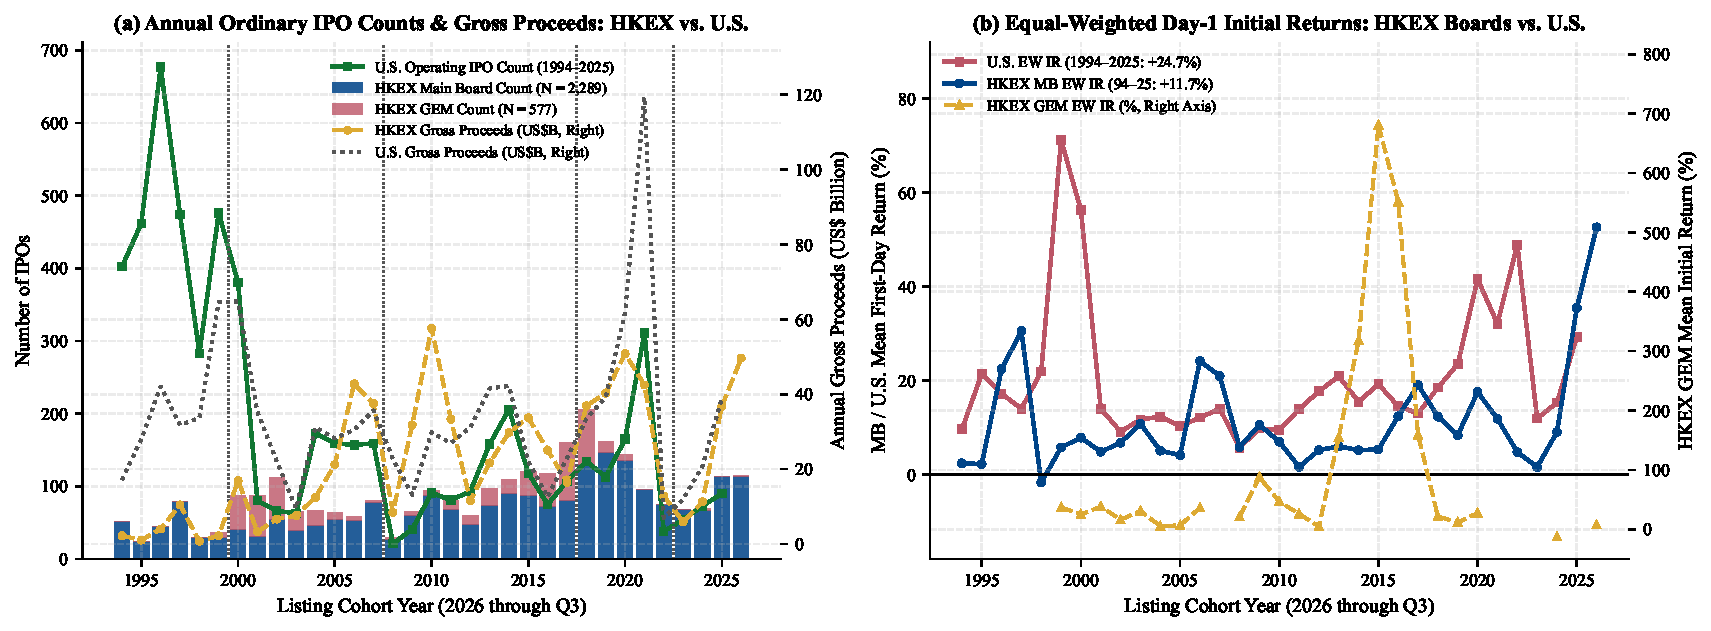
\includegraphics[width=\textwidth,height=0.80\textheight,keepaspectratio]{figures/journal_fig1.pdf}
\caption*{\textbf{Figure 1.1:} Thirty-three years of Hong Kong Main Board and Growth Enterprise Market (GEM) IPO activity paired against U.S. operating-company benchmarks, 1994–2026Q3 ($N = 2,866$ ordinary IPOs on Hong Kong Exchanges and Clearing, HKEX: 2,289 Main Board and 577 GEM). Panel (a) tracks annual HKEX ordinary listing counts and gross proceeds (US\$B) alongside U.S. operating-company IPO counts and proceeds through 2025 from Ritter (2026): while annual U.S. IPO volume fell by roughly three-quarters after 2000 (from 462.3/year in 1994–1999 to 123.3/year in 2000–2025), Hong Kong’s pure Main Board first-time IPOs rose 63\% (from 36.7/year to 59.8/year, alongside 14.0 A+H and 21.9 GEM listings/year). Panel (b) compares annual equal-weighted Day-1 initial returns, $(P_1 - P_0)/P_0$ from offer price $P_0$ to first-day close $P_1$, for HKEX Main Board and U.S. IPOs on the left axis against GEM on a separate, nearly tenfold wider right axis ($N = 2,601$ clean HKEX return records): across 1994–2025 Main Board initial returns averaged +11.7\% (rising to +13.8\% through 2026Q3)—roughly half the U.S. average (+24.7\%) until 2025–2026—whereas GEM surged to +270\%–+742\% during the 2014–2016 placing-only shell boom before collapsing after the February 2018 reform.}
\end{figure}

Four core empirical findings organize the monograph:

\begin{enumerate}
\item \textbf{Cross-System Trust Production, Primary Capital Formation, and Fixed Verification Floors (Sections 2–6).} Hong Kong turned uninvestable cross-border growth into priceable equity by combining a U.S.-dollar currency board, dual Common Law and H-share corporate wrappers, international audits, statutory sponsor liability forged out of repeated crises (1973, 1987, and \textit{Hontex} 2012), and pre-committed cornerstone tranches. Contrary to the concern that offshore IPOs act primarily as insider cash-outs or creditor bailouts, \textbf{83.5\%} of share-verified Main Board offerings sold pure primary shares (97.4\% in 2023–2026), within the 1,862 offerings whose share structure we could verify (HK\$3,428 billion of the census's HK\$5,659 billion), \textbf{94.2\%} of proceeds came from newly issued shares, and only 8.4\% of 214 recent issuers earmarked funds for debt repayment. Producing that cross-border trust carries a steep, indivisible verification floor: while explicit underwriting spreads average just 2.05\%, non-underwriting legal, audit, and sponsor expenses lift mean all-in direct costs from \textbf{3.26\%} in the largest deal quartile to \textbf{17.95\%} in the smallest—screening out small local startups even as Mainland banks rose to sit on nine in ten sponsor teams.
\item \textbf{Price Ceilings, Allocation Rules, and What Applicants Actually Earn (Section 7).} Across all \textbf{1,943} classified offerings with an indicative price range, \textbf{zero} priced above the top of the published offer range, and the gap between first-day close and offer price totals \textbf{HK\$613.6 billion}. When offer-window market news is split at the recorded pricing date, falling markets before pricing pass into first-day returns from the offer price (slope +2.24) while rising markets before pricing do not (-1.43), and news arriving after pricing passes through symmetrically and insignificantly. Offer prices absorb little of a falling market, but positive news does not spill into debut gains as a binding ceiling would predict, so the asymmetry is better read as incomplete downward adjustment than as evidence that the top of the offer range binds. Under Practice Note 18, just above the 15-fold subscription threshold, the retail share of the offer was about 20 percentage points higher (+20.22 pp) and the ratio of the first-day closing price to the offer price was about 22\% lower (-0.247 log points), but the H-share share of issuers also shifts near the threshold, so we treat the drop as an association. After HKEX's August 2025 reform, \textbf{98.0\% (148 of 151)} of eligible non-18C issuers used Mechanism B once six mislabelled prospectuses are corrected; first-day trading volume relative to shares offered was 10 percentage points lower in the before-and-after comparison, a difference that the reform's concurrent bookbuilding and free-float rules prevent us from attributing to Mechanism B alone. Published 2026 allotment schedules ($N = 113$) show what applicants earned: a mean first-day return from the offer price of \textbf{+53.15\%} becomes about \textbf{+1.97\%} net return per dollar applied for on a one-lot cash application (a median gain of HK\$19) and \textbf{-0.06\%} net return per dollar applied for on a Pool B minimum-size financed application ($\ge$ HK\$5M, median fill \textbf{0.11\%}), whose sign depends on how the margin loan is priced. The pattern fits Rock's (1986) rationing, though allocation by order size alone cannot show that informed bidders drove it.
\item \textbf{Entry Price, Screening Gates, and Skewness (Sections 8.1–8.2).} \textbf{77.5\%} of 2,117 split-verified IPOs traded below offer by November 2026, while the shares sold in the 2,116 of them with recorded proceeds gained \textbf{HK\$3.71 trillion} in net price before dividends. The concentration fact is robust: just \textbf{21 companies} generated \textbf{73.8\%} of gross positive gains. Comparisons with a benchmark are more fragile. Defining the \textbf{wealth ratio} as terminal IPO value divided by terminal benchmark value, the ratio against the Hang Seng price index is 1.57; using stock returns with dividends reinvested against an \textit{estimated} dividend-reinvested Hang Seng benchmark the ratio is 1.31, falling to 1.21 if all 475 delistings without terminal quotes are treated as total losses, with a further 274 offerings (HK\$413 billion) outside the analysis because of code or corporate-action problems. Entry price changes the sign of one-year excess returns, +4.9\% from $P_0$ against -4.10\% from the Day-1 close ($N = 1,976$); because $1+R_{P_0} = (1+\text{IR})(1+R_{P_1})$, that reversal measures the first-day return from the offer price itself, not whether secondary buyers overpaid relative to fundamentals. Finally, \textit{weighting by IPO proceeds and board screening} matter: Main Board calendar-time portfolio alphas weighted by IPO proceeds are statistically indistinguishable from zero after adjusting for market, size, momentum, value, and illiquidity, whereas lightly screened GEM suffers persistent negative alphas even under the same five-factor adjustment (-1.27\% per month at 12M). On the Main Board, primary pricing also overlooks pre-IPO accrual quality on Day 1 before low- and high-accrual issuers diverge by 25.6 percentage points over six months.
\item \textbf{A Lasting Local Ecosystem Without Cross-Border Price Integration (Sections 8.3–11).} Listing in Hong Kong inaugurates a continuous financing relationship rather than a one-off cash raise: market-wide follow-on equity by all listed firms exceeded annual IPO proceeds in 16 of 24 benchmark years, roughly half of disclosed listing bills pay for non-underwriting professional services, and HKEX Group's recurring trading, clearing, and data revenues outstrip its listing fees more than elevenfold. These are market and group totals, not amounts attributable to the IPO cohorts in our census. Yet capital-account boundaries and home-market liquidity gravity impose hard limits: Southbound Stock Connect lifted daily trading value (+0.307 log points around automatic A+H admission) and absorbed 25.78\% of A+H float without closing the persistent one-third H-share discount to onshore A-shares, Cayman–PRC lockup gaps reflect issuer-mix drift rather than exposure-scaled expiry selling, and non-Greater-China global brands struggled to retain local secondary trading once listed.
\end{enumerate}

\subsection*{\texorpdfstring{1.2 Theoretical Tension, Hypothesis Development, and Relationship to the Literature}{1.2 Theoretical Tension, Hypothesis Development, and Relationship to the Literature}}
\addcontentsline{toc}{subsection}{\texorpdfstring{1.2 Theoretical Tension, Hypothesis Development, and Relationship to the Literature}{1.2 Theoretical Tension, Hypothesis Development, and Relationship to the Literature}}
We organize the evidence around two bodies of theory: an \textbf{efficiency and institutional-bonding channel} and a \textbf{friction, rationing, and segmentation channel}. The same instruments that make cross-border equity issuance possible (convertible-currency plumbing, statutory sponsor liability, hard offer-price ceilings, retail clawbacks, locked-up cornerstones, and closed-loop trading links) can operate through both at once. A credible disclosure regime can widen access to capital while its fixed compliance cost weighs more heavily on small issuers. Because both channels can hold simultaneously, most of our comparisons do not deliver opposing predictions for the same outcome, and we do not claim to choose between them. We use the two channels as a map of what each test can and cannot show. Where a test does separate them, for example on whether market news passes into offer prices or only into debut prices, we say so; elsewhere the results are descriptive facts about how issuance terms shape investor returns.

\textbf{The Efficiency and Institutional-Bonding Channel.} Under classical law-and-finance and primary-market theory, enforceable legal wrappers, unrestricted currency repatriation, statutory gatekeeper liability, and pre-committed cornerstone investors mitigate cross-border asymmetric information and insider agency risk (La Porta et al., 1998; Coffee, 1999, 2002; Stulz, 1999; Chemmanur and Fulghieri, 1994). By bonding emerging-market issuers to credible disclosure and lowering investor participation barriers—including through retail-access mandates and cross-border trading conduits such as Stock Connect (Merton, 1987)—the market should lower the cost of capital, improve price discovery, broaden liquidity, and narrow cross-market valuation gaps. In long-horizon evaluation, Fama (1998) cautions that abnormal return estimates can depend on portfolio weighting, benchmark choice, and model specification, while Bessembinder (2018) explains how a small number of right-tail winners can account for most cumulative wealth creation even when the median stock underperforms.

\textbf{The Friction, Rationing, and Segmentation Channel.} A complementary set of mechanisms highlights how the rules designed to produce cross-border trust and protect retail investors can introduce binding frictions. First, starting from the partial-adjustment pattern documented in bookbuilding (Benveniste and Spindt, 1989; Hanley, 1993), a statutory ceiling at the top of the published offer range and mandatory retail clawbacks can restrict upward offer-price adjustment and shift excess demand into debut returns and float-scarcity distortions (Derrien, 2005; Ljungqvist, Nanda, and Singh, 2006). Second, under Rock's (1986) winner's-curse equilibrium, uninformed retail applicants are severely rationed out of underpriced issues and disproportionately filled in weak deals, extinguishing scalable economic rents even when first-day returns from the offer price appear lucrative (Koh and Walter, 1989). Third, stringent gatekeeping imposes steep fixed compliance floors that disproportionately burden smaller issuers (Ritter, 1987), while cross-border enforcement remains inherently incomplete (Licht, 2003; Siegel, 2005) and cornerstone tranches may reflect endogenous deal selection and tradable-float compression rather than exogenous certification. Fourth, behavioral market timing, pre-IPO earnings management, and weak junior-board screening expose secondary buyers to persistent post-listing underperformance (Ritter, 1991; Loughran and Ritter, 1995; Teoh, Welch, and Wong, 1998), while non-fungible capital-account borders preserve limits to arbitrage even when trading conduits open (Froot and Dabora, 1999; Jia, Wang, and Xiong, 2017).

Our empirical analysis is organized around \textbf{four sets of comparisons} (summarized in Table 1.1). For each, we state what the two channels would lead one to expect; the final column of Table 1.1 records which comparisons can separate them:

\begin{itemize}
\item \textbf{Hypothesis 1 — Primary Pricing and Allocation: Broad-Access Efficiency vs. Ceiling Distortions and Winner's-Curse Rationing (Section 7).} Under the efficiency and broad-access view (\textit{H1a}), partial adjustment in bookbuilding operates without a binding ceiling distortion—so market news before pricing enters the offer price and first-day close similarly across rising and falling markets—and retail-access rules allow financed subscribers to capture positive net returns per dollar applied for. Under the friction and rationing view (\textit{H1b}), the statutory ceiling at the top of the published offer range prevents pricing above the offer range and creates asymmetric pass-through of market news; mandatory clawback jumps near the 15-fold subscription threshold (and their removal under the August 2025 Mechanism B reform) alter marginal retail supply and first-day trading volume relative to shares offered; and Rock's (1986) adverse-selection rationing drives net returns per dollar applied for on scalable financed orders to zero or below despite elevated first-day returns from the offer price.
\item \textbf{Hypothesis 2 — Gatekeeping and Cornerstones: Credible Bonding and Certification vs. Fixed-Cost Exclusion, Selection, and Float Compression (Sections 5–6).} Under the bonding and certification view (\textit{H2a}), statutory gatekeeping and named, locked-up cornerstone investors credibly screen issuer quality: going-public expenses scale smoothly with deal size, cornerstone backing causally narrows pricing dispersion and improves post-listing survival, and primary pricing impounds pre-IPO accounting quality on Day 1. Under the friction and selection view (\textit{H2b}), compliance verification creates a steep fixed-cost floor that screens out smaller offerings, cornerstone participation reflects endogenous deal selection and assured distribution while compressing tradable float rather than supplying exogenous certification, and differences in pre-IPO accrual quality go unpriced on debut before diverging in aftermarket trading.
\item \textbf{Hypothesis 3 — Long-Horizon Investor Outcomes: Rational Risk Pricing and Right-Tail Compounding vs. Sentiment Overvaluation and Value Destruction (Section 8.1–8.2).} Under the efficient-market and skewness view (\textit{H3a}), once dividends, weighting by IPO proceeds, and seasoned risk factors are properly accounted for, multi-year IPO alphas are indistinguishable from zero and cumulative offered-tranche wealth outperforms passive benchmarks through right-tail compounders. Under the behavioral and agency view (\textit{H3b}), secondary-market buyers who enter at the first-day close systematically overpay during hot issuance windows and suffer persistent negative abnormal returns across listing tiers even after dividend, size, value, and illiquidity adjustments. Testing jointly across entry price ($P_0$ versus $P_1$), portfolio weighting, listing board (Main Board versus GEM), and terminal skewness allows the data to show where each mechanism prevails.
\item \textbf{Hypothesis 4 — Aftermarket Supply and Cross-Border Integration: Investor-Base Convergence vs. Limits to Arbitrage and Supply Frictions (Sections 8.3–8.5).} Under the integration and efficient-supply view (\textit{H4a}), opening Southbound Stock Connect broadens the investor base, simultaneously raising daily trading value and compressing the A–H valuation discount, while predictable statutory lockup expirations are priced ahead of expiry without exposure-scaled sell-offs. Under the segmentation and supply-pressure view (\textit{H4b}), closed-loop, non-fungible capital-account borders allow Stock Connect to expand daily trading value without enabling cross-market arbitrage—leaving the A–H discount intact—while concentrated insider unlocks trigger abnormal price pressure unless staggered by statutory PRC 12-month lockups (Field and Hanka, 2001; Brav and Gompers, 2003).
\end{itemize}

\begin{table}[!htbp]
\centering
\caption*{Table 1.1 — Two Bodies of Theory and the Comparisons Used in This Monograph}
\begin{adjustbox}{max width=\textwidth,max totalheight=0.79\textheight}
\begin{minipage}{\textwidth}\centering
\footnotesize
\setlength{\tabcolsep}{3.5pt}
\renewcommand{\arraystretch}{1.18}
\begin{adjustbox}{max width=\textwidth}
\begin{tabular}{>{\raggedright\arraybackslash}p{2.76cm}>{\raggedright\arraybackslash}p{4.35cm}>{\raggedright\arraybackslash}p{4.35cm}>{\raggedright\arraybackslash}p{4.35cm}}
\toprule
Economic Stage & Efficiency / Bonding Channel ($H_a$) & Friction / Rationing / Segmentation Channel ($H_b$) & Empirical Comparisons, Sections, and Whether They Separate the Channels \\
\midrule
\textbf{H1. Primary Pricing \& Allocation} & Partial adjustment without a binding ceiling distortion; retail access rules let households capture positive net returns per dollar applied for & Statutory ceiling prevents pricing above top of offer range; clawback/Mech. B rules shift retail supply; Rock (1986) rationing eliminates rents on scalable financed orders & Offer-window Hang Seng news split at the pricing date (separates offer-price from debut-price adjustment); PN18 15$\times$ association and Aug 2025 before-and-after comparison (descriptive); 2026 ballot census ($N=113$), net return per dollar applied for \textit{(Section 7)} \\
\textbf{H2. Gatekeeping \& Cornerstones} & Smooth cost scaling; exogenous cornerstone certification narrows dispersion; Day-1 pricing impounds accruals & Regressive fixed compliance floor excludes small deals; cornerstones reflect selection \& float compression; accruals mispriced at debut & Direct cost share by deal quartile ($N=215$); 1,686-placement taxonomy, weak-IV/AR \& Oster bounds; accrual-tercile Day-1 vs. 6M BHR \textit{(Sections 5.3, 6.3, 8.1)} \\
\textbf{H3. Long-Run Wealth \& Pricing} & Zero IPO-proceeds-weighted multi-year alphas; aggregate offered-tranche wealth beats index via right-tail skewness & Persistent negative dividend- and factor-adjusted returns for $P_1$ buyers and weak-screening junior boards & Entry-price ($P_0$ vs. $P_1$) BHARs (linked by the Day-1 return identity); seasoned three-, four-, and five-factor WLS alphas (MB vs. GEM); lifetime skewness (robust) and benchmark wealth ratios (estimated dividend-reinvested Hang Seng benchmark, stated delisting scenarios) \textit{(Sections 8.1–8.2)} \\
\textbf{H4. Lockups \& Cross-Border Links} & Stock Connect lifts daily trading value and closes A–H discount; anticipated lockups cause no expiry drop & Non-fungible Connect expands daily trading value without closing A–H wedge; concentrated unlocks depress prices unless staggered & A+H automatic Connect TWFE DiD ($T_{\text{stab}}+1$) vs. A–H discount path; Cayman vs. PRC Day +180/+240/+365 lockup DiD \& release-fraction tests \textit{(Sections 8.3–8.5)} \\
\bottomrule
\end{tabular}
\end{adjustbox}
\end{minipage}
\end{adjustbox}
\par\vspace{3pt}\noindent\parbox{\textwidth}{\scriptsize\raggedright \textit{Notes}: Synthesis mapping the monograph's comparisons in Sections 5–8 to primary-market, law-and-finance, asset-pricing, and market-segmentation models. The two channels can operate together; only comparisons marked as separating them yield opposing predictions for the same outcome. Abbreviations: \textit{PN18} = Practice Note 18 mandatory retail clawback; \textit{Mech. B} = August 2025 zero-clawback public offer ($\ge 10\%$ initially); \textit{IV / AR} = instrumental variable / Anderson–Rubin; \textit{BHR / BHAR} = buy-and-hold raw / abnormal return; \textit{WLS} = weighted least squares; \textit{MB / GEM} = Main Board / Growth Enterprise Market; \textit{TWFE DiD} = two-way fixed-effects difference-in-differences; \textit{PRC} = People's Republic of China.}
\end{table}

Hanley (1993) documents that IPOs priced above the initial filing range also tend to have higher first-day returns. This pattern motivates a closer look at when information reaches the offer price. Using recorded pricing dates in Hong Kong, we compare how market movements before and after pricing relate to first-day returns. Within the pre-pricing window, we examine rising and falling markets separately and track how far the final offer price moves within the published range.

Agarwal, Liu, and Rhee (2008) link subscription demand to aftermarket performance in Hong Kong, and Vong and Trigueiros (2017) examine how clawback rules affect share allocation and underpricing. Koh and Walter (1989) show why rationing matters when evaluating the returns available to IPO subscribers. We use Hong Kong’s published allotment schedules to compare small cash orders and large financed orders within the same offerings. That comparison measures how fill rates and application costs affect what each strategy earns per dollar applied for.

Coffee (2002) explains how cross-listing can commit issuers to stronger governance standards, while Siegel (2005) examines how those commitments are enforced in practice. Hong Kong offers two institutional arrangements through which to study these commitments: offshore holding companies and mainland-incorporated H-share issuers. We trace the disclosure and enforcement arrangements for each route and use prospectus expense schedules to show how disclosed underwriting and professional fees vary with offering size.

Fama (1998) shows that findings on long-horizon abnormal returns can depend on how those returns are measured. Bessembinder (2018) shows how a small number of stocks can account for a large share of aggregate wealth gains. For Hong Kong IPOs, we compare one-year returns from the offer price and the first-day close for the same offerings. We also measure how much of the cumulative price gain on shares sold at IPO came from the largest winners.

\subsection*{\texorpdfstring{1.3 Data Architecture, Accounting Boundaries, and Roadmap}{1.3 Data Architecture, Accounting Boundaries, and Roadmap}}
\addcontentsline{toc}{subsection}{\texorpdfstring{1.3 Data Architecture, Accounting Boundaries, and Roadmap}{1.3 Data Architecture, Accounting Boundaries, and Roadmap}}
Standard vendor downloads systematically distort historical Hong Kong IPO series by commingling non-capital-raising introductions, GEM-to-Main-Board transfers, investment vehicles, and SPACs with genuine operating IPOs, while leaving recycled tickers, unadjusted share consolidations, missing delisting exits, and blank fee schedules uncorrected (Appendix A details our full diagnostic audit and reconciliation waterfall). To match empirical claims strictly to what historical disclosures permit, we organize the evidence across \textbf{three nested empirical lenses} (Table 1.2)—spanning the complete 33-year census ($N = 2,866$), modern post-2018 and 2025–2026Q3 filing-level microdata ($N = 943$ and $N = 226$), and the exact 2026 retail ballot corpus ($N = 113$)—while separating structural cross-sectional mechanisms from cyclical Era V market heat.

\begin{table}[!htbp]
\centering
\caption*{Table 1.2 — Nested Sample Architecture: Population, Subsamples, Unit of Observation, and Off-Census Ledger}
\begin{adjustbox}{max width=\textwidth,max totalheight=0.79\textheight}
\begin{minipage}{\textwidth}\centering
\footnotesize
\setlength{\tabcolsep}{3.5pt}
\renewcommand{\arraystretch}{1.18}
\begin{adjustbox}{max width=\textwidth}
\begin{tabular}{>{\raggedright\arraybackslash}p{4.39cm}>{\centering\arraybackslash}p{3.19cm}>{\centering\arraybackslash}p{4.11cm}>{\raggedright\arraybackslash}p{4.11cm}}
\toprule
Empirical Lens & Observation Window & Core Sample ($N$) & Primary Analytical Scope \& Disclosure Rationale \\
\midrule
\textbf{1. 33-Year Population Census} \textit{(Full Population)} & Jan 1994 – Sep 2026 \textit{(Cutoff Nov 12, 2026)} & \textbf{2,866} ordinary IPOs \textit{(2,289 MB / 577 GEM; 2,601 clean Day-1; 1,976 1Y MB; 2,117 terminal)} & Macro issuance waves, syndicate shares, hard price ceilings, PN18 clawbacks, FINI HIBOR cycles, 1Y–3Y returns, liquidity decay, and lifetime wealth \\
\textbf{2. Modern Track \& Micro-Contracting Corpus} \textit{(Subset of Lens 1 MB)} & Jan 2018 – Sep 2026 \& \textbf{2025Q1–2026Q3} & \textbf{943} modern MB tracks; within it, \textbf{226} closely reviewed MB deals \textit{(215–216 fee schedules; 1,686 cornerstones)} & Post-2018 Ch. 8A/18A/18C/19C gateways; itemized legal/audit vs. underwriting fees, VC/PRC guidance equity, R\&D \& accruals, lockups, and Mechanism B \\
\textbf{3. Retail Ballot Census} \textit{(Subset of Lens 2 226)} & Jan 2026 – Sep 2026 & \textbf{113} Main Board IPOs & Published allotment-schedule Pool A (1-lot, 10-lot) and Pool B ($\ge$ HK\$5M) fill rates and net FINI margin returns testing Rock (1986) \\
\textbf{Off-Census Historical Ledger} \textit{(Separate Non-Overlapping Set)} & 1891 – 2026 & \textbf{Appendix B} & Pre-1994 milestones, ETFs/REITs (\textit{TraHK}, \textit{Link}), introductions (\textit{0388.HK}), and halted/diverted deals (\textit{Ant Group}, \textit{Alibaba 2014}) kept outside operating-IPO denominators \\
\bottomrule
\end{tabular}
\end{adjustbox}
\end{minipage}
\end{adjustbox}
\par\vspace{3pt}\noindent\parbox{\textwidth}{\scriptsize\raggedright \textit{Notes}: \textit{Unit of observation}: the individual ordinary operating-company IPO offering (except the 1,686 investor-deal cornerstone placements nested inside Lens 2's 226 deals, and historical events in Appendix B). \textit{Sample nesting}: Lens 1 ($N = 2,866$: 2,289 Main Board [MB] and 577 Growth Enterprise Market [GEM] IPOs on Hong Kong Exchanges and Clearing [HKEX]) is the full population; clean Day-1 ($N = 2,601$), matured 1-year Main Board ($N = 1,976$), and split-verified terminal ($N = 2,117$) panels are filtered subsets of Lens 1 (Appendix A). Lens 2 is a strict Main Board subset of Lens 1 ($943 \subset 2,289$, with $226 \subset 943$ closely reviewed 2025Q1–2026Q3 deals), and Lens 3 is a strict 2026 subset of Lens 2 ($113 \subset 226$). The Off-Census Historical Ledger (Appendix B) is a separate, non-overlapping reference catalogue compiled from exchange, regulatory, and court records (cross-referencing in-census MTR 0066.HK as a public-asset comparator). Abbreviations: \textit{PN18} = Practice Note 18 mandatory retail clawback; \textit{FINI} = Fast Interface for New Issuance; \textit{HIBOR} = Hong Kong Interbank Offered Rate; \textit{Ch. 8A / 18A / 18C / 19C} = Main Board listing routes for weighted voting rights, pre-revenue biotech, pre-commercial specialist technology, and secondary listings; \textit{VC} = venture capital; \textit{PRC} = People's Republic of China; \textit{Mechanism B} = August 2025 fixed-tranche public offer with zero clawback; \textit{ETF / REIT} = exchange-traded fund / real estate investment trust. \textit{Source}: Appendix A Sample Waterfall and Appendix B Off-Census Ledger.}
\end{table}

Throughout, we enforce explicit accounting boundaries: gross IPO proceeds (HK\$5,659.4 billion) measure the total value of shares sold at IPO, including shares sold by existing holders, rather than new capital or Hong Kong GDP; the new-share share of proceeds (94.2\%) is measured only in the 1,862 offerings with verified share structures, and follow-on issuance and HKEX revenue are market- or group-level series that are not attributed to the census cohorts (where C\&SD financial-services value added of HK\$816.2 billion, or 26.2\% of 2024 nominal GDP, provides urban context rather than IPO-caused attribution); benchmarked post-listing returns (Section 8.1) are kept distinct from cumulative offered-tranche wealth (Section 8.2); retail ballot returns always state whether denominators are allotted shares or pledged margin capital (Section 7.4); and non-IPO milestones (\textit{Tracker Fund}, \textit{Link REIT}, \textit{HKEX} introduction, \textit{Ant Group} halt) are tracked separately in Appendix B.

The monograph follows a clear economic logic. Credible currency convertibility, enforceable shareholder protections, and statutory gatekeeping should lower the barriers to cross-border equity investment—yet the fixed verification and compliance costs required to produce that trust weigh disproportionately on smaller offerings, whose capital-flow and cost consequences appear first in Section 5. The chapters unfold in three parts:

\begin{itemize}
\item \textbf{Part I (Sections 2–4)} explains which issuing institutions Hong Kong built: the monetary, legal, and agglomeration foundations of cross-border trust (Section 2); the crisis-driven evolution from colonial bourses to central clearing, 1891–1993 (Section 3); and the five modern issuance eras plus stalled and diverted deals, 1994–2026 (Section 4).
\item \textbf{Part II (Sections 5–8)} traces how listing, pricing, and trading rules shape outcomes for each party: issuer capital flows, listing tracks, fixed compliance costs, and follow-on financing (Section 5); sponsors, syndicates, cornerstones, and statutory enforcement (Section 6); price ceilings, clawbacks, margin financing, and stabilization (Section 7); and aftermarket one-year returns, lifetime wealth concentration, lockups, liquidity decay, and Stock Connect (Section 8).
\item \textbf{Part III (Sections 9–12)} tracks where the gains and economic activity ultimately landed: retained urban value in Hong Kong (Section 9); Mainland corporate governance and proceeds-to-operations trajectories (Section 10); global investor origins and non-Mainland international listings (Section 11); and era-by-era counterfactuals, trade-offs, broader finance implications, and stakeholder takeaways (Section 12).
\end{itemize}

Together, the three parts return to a single question: how did Hong Kong make cross-border equity issuance possible at scale, and how did the gains and costs fall across issuers, investors, and the city itself?

\par\vspace{16pt}\needspace{9\baselineskip}
\noindent\rule{\linewidth}{0.85pt}\par\vspace{5pt}
{\centering\Large\bfseries\color{NavyAccent} \texorpdfstring{PART I — THE MAKING OF THE MARKET (1891–2026)}{PART I — THE MAKING OF THE MARKET (1891–2026)}\par}
\vspace{4pt}\noindent\rule{\linewidth}{0.85pt}\par\vspace{8pt}
\addcontentsline{toc}{section}{\texorpdfstring{\textbf{PART I — THE MAKING OF THE MARKET (1891–2026)}}{PART I — THE MAKING OF THE MARKET (1891–2026)}}
\section*{\texorpdfstring{Section 2. Why Hong Kong? The Foundations of a Cross-Border Equity Market}{Section 2. Why Hong Kong? The Foundations of a Cross-Border Equity Market}}
\addcontentsline{toc}{section}{\texorpdfstring{Section 2. Why Hong Kong? The Foundations of a Cross-Border Equity Market}{Section 2. Why Hong Kong? The Foundations of a Cross-Border Equity Market}}
\markright{Section 2. Why Hong Kong? The Foundations of a...}
Why did Mainland Chinese enterprises and international institutional investors converge in Hong Kong rather than onshore in Shanghai and Shenzhen or in rival offshore centers such as Singapore and London? The economic problem is deeper than geographic proximity. An ordinary share carries no maturity date and no pledged collateral; buying equity across a political and legal border requires handing cash today in exchange for a residual claim on profits earned inside another jurisdiction, managed by insiders whom minority shareholders cannot easily remove (La Porta et al., 1998; Stulz, 1999). Any cross-border investor therefore demands credible answers to three practical questions before writing a check: \textit{can proceeds and dividends be repatriated without exchange controls, can minority shareholder rights be enforced, and who is held accountable if a prospectus misstates the facts?} In the early 1990s, Mainland China possessed capital-hungry industrial enterprises, yet operated behind capital-account controls with a non-convertible currency and an incomplete company-law regime. International pension and mutual funds held deep, low-cost capital, yet required internationally audited financial statements, unrestricted currency repatriation, and a credible judicial and regulatory backstop.

Hong Kong bridged this divide by combining four elements: a U.S.-dollar currency board guaranteeing capital convertibility, adaptable legal wrappers separating operating assets from corporate governance, a tripartite cross-border supervisory structure, and dense professional agglomeration capable of turning Mainland commercial operations into standardized prospectuses. None of these foundations was built in advance for Mainland capital raising; each emerged from an earlier local crisis, which is why the pre-1993 institutional history in Section 3 matters.

\subsection*{\texorpdfstring{2.1 Monetary Credibility and the Currency Board}{2.1 Monetary Credibility and the Currency Board}}
\addcontentsline{toc}{subsection}{\texorpdfstring{2.1 Monetary Credibility and the Currency Board}{2.1 Monetary Credibility and the Currency Board}}
Cross-border equity investment begins with repatriation certainty: no foreign portfolio manager will commit long-term equity capital if dividends or liquidation proceeds risk being trapped behind exchange controls. Forged during the 1983 confidence crisis over Hong Kong's political transition, the Linked Exchange Rate System pegs the Hong Kong dollar to the U.S. dollar under a currency board with full foreign-exchange backing and no capital controls, a framework preserved across the 1997 handover.\footnote{After the Hong Kong dollar slid to HK\$9.60 per U.S. dollar in September 1983 during Sino-British negotiations, the government instituted the Linked Exchange Rate System on October 17, 1983 at HK\$7.80 per U.S. dollar, later refined into the HK\$7.75–7.85 convertibility band. Articles 109–112 of the Basic Law (promulgated in 1990) carried full foreign-exchange backing and the prohibition on capital controls across the 1997 handover.}

Convertibility carries a well-defined macroeconomic trade-off. Under open capital flows and a fixed exchange rate, Hong Kong imports U.S. Federal Reserve monetary cycles and global dollar funding costs (the Mundell–Fleming trilemma). Large cross-border IPO subscriptions also transmit directly into short-term domestic interbank funding rates, a link we examine alongside settlement reform in Section 7.3. Yet a convertible currency alone protects no shareholder from inflated revenues or insider tunneling; monetary credibility was a necessary floor, while corporate credibility required legal and supervisory engineering.

\subsection*{\texorpdfstring{2.2 Legal Wrappers and Tripartite Cross-Border Governance}{2.2 Legal Wrappers and Tripartite Cross-Border Governance}}
\addcontentsline{toc}{subsection}{\texorpdfstring{2.2 Legal Wrappers and Tripartite Cross-Border Governance}{2.2 Legal Wrappers and Tripartite Cross-Border Governance}}
Answering the second and third investor questions—whether minority shareholder rights can be enforced and who answers if a prospectus misstates the facts—required separating three attributes that domestic markets normally fuse: \textbf{where the enterprise operates}, \textbf{where its legal entity is incorporated}, and \textbf{who polices its disclosure}. In the cross-listing literature, this separation enables emerging-market issuers to bond themselves to stricter disclosure and enforcement abroad (Coffee, 1999, 2002; Stulz, 1999), though cross-border enforcement against controlling insiders remains inherently incomplete (Licht, 2003; Siegel, 2005).

Two legal wrappers operationalized that separation (Table 2.1). The \textbf{offshore corridor} allowed Hong Kong and Mainland businesses to list through holding companies incorporated in Common Law jurisdictions—first Bermuda and later predominantly the Cayman Islands, including private internet firms using contractual Variable Interest Entity (VIE) structures such as Tencent. The \textbf{H-share corridor} left legal incorporation inside the People's Republic of China while writing Common Law minority protections, international audits, and cross-border dispute safeguards directly into corporate charters under Chapter 19A of the Listing Rules. In short, the offshore corridor moved the issuer to the law, whereas the H-share corridor brought the law to the issuer.

Disclosure accountability rested on a \textbf{tripartite supervisory structure} (Table 2.1): frontline listing vetting by \textbf{Hong Kong Exchanges and Clearing (HKEX)}, statutory oversight and enforcement by the independent \textbf{Securities and Futures Commission (SFC)}, and onshore asset, foreign-exchange, and overseas-listing filing authority retained by \textbf{Mainland Chinese regulators}. Across both corridors, the prospectus is the binding legal interface subjecting directors and intermediaries to Hong Kong statutory liability regardless of where physical factories sit. That accountability was tested publicly in \textit{Hontex} (2012), when the SFC obtained a court order requiring roughly HK\$1 billion in investor restitution for fabricated prospectus financials and sanctioned the deal's sponsor—leading directly to stricter statutory sponsor diligence standards (Section 6.4).

\begin{table}[!htbp]
\centering
\caption*{Table 2.1 — Cross-Border Legal Wrappers, Disclosure Oversight, and Key Institutional Amendments}
\begin{adjustbox}{max width=\textwidth,max totalheight=0.79\textheight}
\begin{minipage}{\textwidth}\centering
\footnotesize
\setlength{\tabcolsep}{3.5pt}
\renewcommand{\arraystretch}{1.18}
\begin{adjustbox}{max width=\textwidth}
\begin{tabular}{>{\raggedright\arraybackslash}p{3.91cm}>{\raggedright\arraybackslash}p{5.80cm}>{\raggedright\arraybackslash}p{5.80cm}}
\toprule
Institutional Layer & Core Mechanism & Detailed Charter / Rule Provisions \& Historical Revisions \\
\midrule
\textbf{Offshore Holding Corridor} & Issuer incorporates in Common Law domicile (\textit{Bermuda}, \textit{Cayman Islands}) while operating in Mainland China or Hong Kong & Precedent set by Jardine Matheson's 1984 Bermuda redomiciliation; Cayman Islands became the primary private-enterprise wrapper, including contractual VIE structures (\textit{Tencent}, 2004). \\
\textbf{PRC H-Share Corridor (Chapter 19A)} & Issuer remains PRC-incorporated while embedding minority protections in its corporate charter & Built on the June 1993 MoU and August 1994 \textit{Mandatory Provisions}: separate H-share class voting vetoes, connected-transaction approvals, IFRS/HKFRS audits, and Hong Kong or international arbitration. China repealed the \textit{Mandatory Provisions} in March 2023 under its unified overseas-listing filing regime; HKEX streamlined Chapter 19A accordingly, with existing charter protections remaining binding until amended. \\
\textbf{Frontline \& Statutory Oversight} & Dual-layer Hong Kong supervision paired with Mainland onshore authority & \textbf{HKEX} (demutualized and self-listed in June 2000) conducts frontline vetting; the independent \textbf{SFC} exercises concurrent prospectus review under the April 2003 dual-filing regime and statutory enforcement (e.g., \textit{Hontex} 2012 restitution and October 2013 Paragraph 17 sponsor rules); \textbf{Mainland authorities} (CSRC and sectoral ministries) control onshore assets, FX approvals, and post-March 2023 overseas-listing filings (evidenced by the November 2020 \textit{Ant Group} halt). \\
\bottomrule
\end{tabular}
\end{adjustbox}
\end{minipage}
\end{adjustbox}
\par\vspace{3pt}\noindent\parbox{\textwidth}{\scriptsize\raggedright \textit{Notes}: Compact institutional reference supporting Section 2.2. Abbreviations: \textit{PRC} = People's Republic of China; \textit{VIE} = Variable Interest Entity; \textit{MoU} = Memorandum of Regulatory Cooperation; \textit{IFRS / HKFRS} = International / Hong Kong Financial Reporting Standards; \textit{HKEX} = Hong Kong Exchanges and Clearing; \textit{SFC} = Securities and Futures Commission; \textit{CSRC} = China Securities Regulatory Commission; \textit{FX} = foreign exchange. \textit{Source}: HKEX Listing Rules (Chapter 19A), SFC Dual-Filing and Enforcement Releases, and Cha (2023).}
\end{table}

\subsection*{\texorpdfstring{2.3 Agglomeration, Institutional Production, and Positional Arbitrage}{2.3 Agglomeration, Institutional Production, and Positional Arbitrage}}
\addcontentsline{toc}{subsection}{\texorpdfstring{2.3 Agglomeration, Institutional Production, and Positional Arbitrage}{2.3 Agglomeration, Institutional Production, and Positional Arbitrage}}
Currency stability and legal architecture still require specialized human capital to operate at scale (Allen, Qian, and Qian, 2005). Hong Kong concentrated investment bankers, cross-border securities lawyers, Big-4 reporting accountants, valuers, financial printers, and regulators within a few blocks of Central, generating \textbf{dual proximity}—combining operational familiarity with Mainland firms and officials with international legal and fiduciary standards. As background context, peer Common Law centers with open capital accounts such as Singapore (which hosted a 2000s wave of Mainland ``S-Chip'' listings later hit by accounting scandals) and London (Alternative Investment Market foreign listings) did not sustain comparable cross-border Chinese issuance, even though Hong Kong faced its own accounting failures such as \textit{Hontex} (2012). Cross-center comparisons cannot isolate which single institution caused differences in listing volume, because proximity, regulatory enforcement, investor clientele, and Beijing's policy choices moved together.

A financial history must therefore keep \textbf{institutional production} distinct from \textbf{positional arbitrage}. Hong Kong's currency board, adaptable legal wrappers, statutory gatekeeping, and professional cluster lowered the cost of cross-border contracting. Yet issuance volume also depended on asymmetries outside the city's control: a closed Mainland capital account, administratively rationed onshore A-share queues (Qian, Ritter, and Shao, 2024), and Beijing's decision since 1993 to channel external equity formation through Hong Kong. Keeping those two forces distinct frames our interpretation of returns (Part II), host-city value (Section 9), and counterfactual alternatives (Section 12).

\subsection*{\texorpdfstring{2.4 Why Hong Kong Matters Beyond Hong Kong: Direct Observation of IPO Allocation}{2.4 Why Hong Kong Matters Beyond Hong Kong: Direct Observation of IPO Allocation}}
\addcontentsline{toc}{subsection}{\texorpdfstring{2.4 Why Hong Kong Matters Beyond Hong Kong: Direct Observation of IPO Allocation}{2.4 Why Hong Kong Matters Beyond Hong Kong: Direct Observation of IPO Allocation}}
The monetary, legal, and supervisory foundations above explain why Hong Kong became a major cross-border listing center. A distinct institutional feature explains why Hong Kong's data also speak directly to a universal question in international IPO research: \textbf{when offerings with larger first-day gains are harder to receive shares in, how much does the average first-day return overstate the return on an actual application strategy?}

For any given application tier, the gross return per dollar applied for equals the \textbf{fill rate} (shares allotted divided by shares applied for) multiplied by the \textbf{first-day return from the offer price}, $(P_1 - P_0)/P_0$. Whenever fill rates are systematically lower in offerings that jump most on debut, negative covariance between allocation and initial return compresses the average gross return per dollar applied for well below the first-day return from the offer price (Rock, 1986). Empirical evidence from the United States shows that institutional allocations correlate systematically with first-day returns under discretionary bookbuilding (Aggarwal, Prabhala, and Puri, 2002), while Singapore's fixed-price rationing data provided an early test of Rock's prediction (Koh and Walter, 1989). Hong Kong extends this literature by letting us measure, within the \textit{same} batch of modern bookbuilt offerings, how order size and margin financing terms alter the return achievable by different investor tiers. What generalizes beyond Hong Kong is this economic mechanism—how rationing covariance, order scale, and funding costs separate first-day returns from the offer price from net returns per dollar applied for—whereas the exact return magnitudes depend on each market's allocation rules, transaction charges, and financing terms.

IPO underpricing measures the first-day gain on an allocated share. The payoff to submitting an order also depends on how many shares the investor receives and what it costs to apply. Hong Kong’s published allotment schedules report the shares applied for and allotted at different order sizes. They allow us to compare small cash applications and large financed applications within the same offerings, holding the offer price and first-day closing price fixed. When allocations are smaller in deals with larger debut gains, rationing reduces the return per dollar applied for. The same question arises in markets where underwriters allocate shares at their discretion, including the United States. Hong Kong’s disclosures let us measure separately how fill rates, order size, and financing terms contribute to the returns of specified application strategies.

\par\medskip\noindent\rule{\linewidth}{0.35pt}\par\medskip
\section*{\texorpdfstring{Section 3. From Trading Port to Financial Infrastructure, 1891–1993}{Section 3. From Trading Port to Financial Infrastructure, 1891–1993}}
\addcontentsline{toc}{section}{\texorpdfstring{Section 3. From Trading Port to Financial Infrastructure, 1891–1993}{Section 3. From Trading Port to Financial Infrastructure, 1891–1993}}
\markright{Section 3. From Trading Port to Financial Infra...}
The prehistory answers one question: \textbf{when Mainland enterprises finally came looking for foreign capital in 1993, why was Hong Kong ready to receive them?} It was not ready because the market had grown smoothly. For most of its first century the exchange served a narrow clientele, played little part in financing local industry, and failed spectacularly more than once. The readiness came from those failures. The 1973 crash brought securities law. The 1987 closure brought an independent regulator. Settlement backlogs brought central clearing. By 1993 a speculative local market had been rebuilt, crisis by crisis, into something an international investor could use.

\subsection*{\texorpdfstring{3.1 A Club That Did Not Finance the Factories (1891–1968)}{3.1 A Club That Did Not Finance the Factories (1891–1968)}}
\addcontentsline{toc}{subsection}{\texorpdfstring{3.1 A Club That Did Not Finance the Factories (1891–1968)}{3.1 A Club That Did Not Finance the Factories (1891–1968)}}
Formal share trading began in February 1891, when mostly expatriate brokers formed the Association of Stockbrokers in Hong Kong, renamed the Hong Kong Stock Exchange in 1914. Rapid postwar-WWI shipping, rubber, and property speculation led rival brokers to form the Hong Kong Stockbrokers' Association in 1921, creating a pre-war duopoly (HKEX, 2000 listing document). Trading stopped under Japanese occupation (1941–1945), and the two bodies merged on March 3, 1947. What emerged was an orderly but narrow, English-speaking market centered on British-linked trading houses, utilities, banks, and property developers.

Then came one of the most striking episodes in the city's economic history. After 1949, refugee industrialists, many of them Shanghai textile families, turned Hong Kong into a global export manufacturer. And the stock exchange had almost nothing to do with it. Factories were financed by retained family profit and, above all, by commercial bank credit, with HSBC at the center.

Why banks and not the bourse? Export orders turned over quickly against letters of credit, which made them natural short-term bank collateral. Family owners valued secrecy and control and saw little reason to share equity while overdraft lines kept rolling. Meanwhile the merged exchange maintained high seat barriers, conducted floor business in English, and offered little secondary liquidity for mid-sized manufacturers. Long-lived infrastructure such as power plants and docks used the equity market; working capital stayed with the banks. This matches standard finance-and-growth theory (Rajan and Zingales, 1998; Levine, 2005) and sets up the rest of the story: on the eve of the 1970s, Hong Kong had a booming industrial economy and a stock market most of its residents never touched.

\subsection*{\texorpdfstring{3.2 Democratization, Mania, and the First Lesson in Regulation (1969–1986)}{3.2 Democratization, Mania, and the First Lesson in Regulation (1969–1986)}}
\addcontentsline{toc}{subsection}{\texorpdfstring{3.2 Democratization, Mania, and the First Lesson in Regulation (1969–1986)}{3.2 Democratization, Mania, and the First Lesson in Regulation (1969–1986)}}
Two decades of manufacturing growth had put savings in Chinese hands, and a new generation of property developers wanted permanent equity capital. The incumbent exchange served neither group well. In December 1969, Ronald Li and local Chinese brokers opened the Far East Exchange, introducing Cantonese trading and smaller board-lot denominations that cut minimum cash tickets for salaried households. The Kam Ngan (1971) and Kowloon (1972) exchanges soon followed, giving the city four competing trading floors. Share ownership became a mass pursuit, and the listings of 1972–1973, led by Cheung Kong and its peers, gave Chinese developers listed equity currency to rival the British \textit{hongs}. Within a decade Cheung Kong would control Hutchison Whampoa and Y.K. Pao would control Wheelock.

Multiple competing exchanges also showed how quickly standards erode when entry venues race for volume. Four broker-owned exchanges competed aggressively for new listings, broker margin credit expanded unchecked, and Hong Kong still had no independent securities regulator. A surge of unseasoned new issues pushed the Hang Seng Index to 1,774.96 in March 1973. Forged share certificates surfaced during paper settlement, interest rates jumped, the oil shock hit, and by December 1974 the index stood at 150.11, a collapse of 91.5\%.

The crash produced the first lasting statutory response to unregulated listing competition. The Securities Ordinance and the Protection of Investors Ordinance of 1974 ended pure \textit{laissez-faire} by creating a formal supervisory framework, and unification legislation pressed the four exchanges to merge. Meanwhile, the 1983 Linked Exchange Rate System resolved currency-repatriation risk by pegging the Hong Kong dollar to the U.S. dollar (Section 2.1). On April 2, 1986 the four floors combined into the Stock Exchange of Hong Kong inside Exchange Square, ending fragmented venue competition—though the structural lesson that competing listing venues without an independent gatekeeper erode standards first and punish retail buyers later would be relearned on GEM four decades on.

\subsection*{\texorpdfstring{3.3 1987 and the Rebuilding That Made H-Shares Possible}{3.3 1987 and the Rebuilding That Made H-Shares Possible}}
\addcontentsline{toc}{subsection}{\texorpdfstring{3.3 1987 and the Rebuilding That Made H-Shares Possible}{3.3 1987 and the Rebuilding That Made H-Shares Possible}}
Unifying the trading floor ended venue fragmentation, but left governance unresolved. Two episodes in 1987 forced structural reform, followed by an operational overhaul of clearing and settlement.

First, minority voting rights were tested in March 1987, when Cheung Kong, Hutchison, and Jardine Matheson proposed ``B shares'' that would give controlling holders votes at a fraction of the economic cost. Investors objected, prices fell, and regulators intervened. Proportional voting was then written into the listing rules (Rule 8.11), protecting minority investors against entrenched control for three decades before costing Hong Kong the Alibaba IPO (Section 4.3).

Seven months later, broker-guild capture broke open. After Wall Street crashed on October 19, the leveraged futures market threatened to exhaust its clearing guarantee, and the exchange, under Ronald Li, closed the stock and futures markets for four trading days. When trading resumed, the Hang Seng fell by a third in one session, requiring a rescue package of about HK\$4 billion. The Hay Davison report of 1988 described an exchange run as an inside club. Its remedy was structural: the Securities and Futures Commission opened in 1989 as an independent statutory regulator, exchange governance was broadened, and risk management was rebuilt.

Clearing capacity posed the final operational bottleneck. Trading still depended on moving paper certificates between brokers and registrars, and volume spikes caused backlogs and forgery risks. The Central Clearing and Settlement System (CCASS) began in June 1992, and automatic order matching (AMS) arrived in November 1993, giving a market that had nearly stalled in 1987 the capacity to clear large international offerings.

This is the point at which the local story met the national one, resolving the cross-border legal-domicile gap. After Deng Xiaoping's 1992 Southern Tour, Mainland leaders sought foreign equity capital and modern corporate discipline for state enterprises without giving up onshore legal domicile. Vice Premier Zhu Rongji backed the effort, and Liu Hongru led the Mainland delegation alongside a Hong Kong team that included Charles Lee, Herbert Hui, and Laura Cha (Cha, 2023). The legal gap was daunting: China had no national Company Law (adopted only in December 1993, effective July 1994), and H-shares remained non-fungible with domestic state-held shares. Negotiators bridged that gap by contractual governance rather than waiting for cross-border statutory convergence. A Memorandum of Regulatory Cooperation was signed in June 1993, Hong Kong inserted Chapter 19A into its Listing Rules, and each issuer wrote enforceable minority safeguards (equal dividend rights, separate H-share class vetoes, international financial reporting audits, and Hong Kong or international arbitration for shareholder disputes) directly into its articles of association, standardized in the \textit{Mandatory Provisions} of August 1994. Internally, candidate state enterprises had to carve operating assets out of cradle-to-grave \textit{danwei} units (schools, hospitals, employee housing) before restating three years of accounts.

On July 15, 1993, Tsingtao Brewery began trading as the first H-share. Each ingredient had solved a specific constraint forged by an earlier crisis: the 1983 currency board removed repatriation risk; the 1989 SFC ended broker self-regulation; Rule 8.11 protected minority votes; CCASS and AMS broke paper settlement bottlenecks; and Chapter 19A bridged PRC legal domicile. \textbf{Hong Kong was ready in 1993 largely because it had already paid for its mistakes.} Section 4 traces how that 1993 bridge expanded and was repeatedly rebuilt over the next thirty-three years.

\begin{table}[!htbp]
\centering
\caption*{Table 3.1 — Institutional and Infrastructure Chronology of the Pre-Modern Market, 1891–1993}
\begin{adjustbox}{max width=\textwidth,max totalheight=0.79\textheight}
\begin{minipage}{\textwidth}\centering
\footnotesize
\setlength{\tabcolsep}{3.5pt}
\renewcommand{\arraystretch}{1.18}
\begin{adjustbox}{max width=\textwidth}
\begin{tabular}{l>{\raggedright\arraybackslash}p{4.83cm}>{\raggedright\arraybackslash}p{4.83cm}>{\raggedright\arraybackslash}p{4.83cm}}
\toprule
Year / Date & Institutional / Infrastructure Milestone & Governance \& Market Plumbing Shift & Real-Economy \& Cross-Border Significance \\
\midrule
\textbf{Feb 1891 / 1914} & \textit{Association of Stockbrokers} founded (HKSE in 1914) & Expatriate guild outcry floor on Ice House Street & Trades colonial \textit{hongs}, shipping, docks, banks, and utilities \\
\textbf{1921 – Mar 1947} & Rival \textit{HK Stockbrokers’ Association} (1921), WWII closure (1941–45), merger (Mar 3, 1947) & Pre-war duopoly consolidated into post-war \textit{HKSE} & Post-1949 Shanghai textile/export industry financed by \textbf{HSBC bank credit}, bypassing the stock market \\
\textbf{Dec 1969 – Jan 1972} & \textit{Far East (1969)}, \textit{Kam Ngan (1971)}, and \textit{Kowloon (1972)} exchanges open & Cantonese outcry, smaller board lots, four competing floors & Democratizes retail share ownership; launches \textbf{Class of 1972} Chinese property giants (\textit{Cheung Kong}, \textit{SHKP}, \textit{New World}) \\
\textbf{Mar 1973 – Dec 1974} & HSI crashes \textbf{91.5\%} (1,774.96 $\to$ 150.11); \textit{Securities Ordinance (1974)} & Ends regulatory \textit{laissez-faire}; creates part-time Securities Commission & Exposes race-to-the-bottom listing competition (a surge of new issues) and forged paper scrip \\
\textbf{Oct 17, 1983} & \textbf{Linked Exchange Rate System (LERS, HK\$7.80/USD)} & Currency board eliminates FX/repatriation risk (enshrined in 1990 Basic Law Arts. 109–112) & Anchors international USD institutional confidence across the 1997 transition; imports US Fed rate cycles into HIBOR \\
\textbf{Apr 2, 1986} & \textbf{Unified Stock Exchange of Hong Kong (SEHK)} opens & Merges the four private exchanges into one Exchange Square floor & Centralizes liquidity, though governance remains broker-dominated \\
\textbf{Mar \& Oct 1987} & \textbf{B-Share revolt} (Mar) \& \textbf{4-day Black Monday closure} (Oct 20–23) & Triggers \textbf{Hay Davison Report (May 1988)}, \textbf{SFC (May 1989)}, and \textbf{Rule 8.11 (1-share-1-vote, 1989)} & Replaces broker-guild capture with statutory independent oversight and strict voting proportionality \\
\textbf{Jun 1992 \& Nov 1993} & \textbf{CCASS (Jun 1992)} paperless depository \& \textbf{AMS (Nov 1993)} matching & Eliminates physical certificate vans; digitizes order matching & Gives Hong Kong industrial-scale clearing and trading capacity \\
\textbf{Jun–Jul 15, 1993} & \textbf{MoU, Chapter 19A, \& Tsingtao Brewery (0168.HK) IPO} & Bilateral legal graft (charter safeguards, IAS audit, class vetoes; standardized in the 1994 \textit{Mandatory Provisions}) & Opens the modern cross-border equity bridge for Mainland China \\
\bottomrule
\end{tabular}
\end{adjustbox}
\end{minipage}
\end{adjustbox}
\par\vspace{3pt}\noindent\parbox{\textwidth}{\scriptsize\raggedright \textit{Notes}: Institutional chronology compiled from Hong Kong Exchanges and Clearing (HKEX) historical archives, the Hay Davison Report (1988), Securities and Futures Commission (SFC) records, and Hong Kong Basic Law Articles 109–112. Each milestone documents the specific cross-border financing or market-integrity friction—currency convertibility (anchoring Hong Kong Interbank Offered Rate [HIBOR] cycles), broker self-regulation, physical settlement congestion, or cross-jurisdictional charter governance—resolved before the 1994 modern IPO census opens. Abbreviations: \textit{HKSE} = Hong Kong Stock Exchange; \textit{SEHK} = Stock Exchange of Hong Kong; \textit{HSI} = Hang Seng Index; \textit{CCASS} = Central Clearing and Settlement System; \textit{AMS} = Automatic Order Matching and Execution System; \textit{IAS} = International Accounting Standards; \textit{MoU} = Memorandum of Regulatory Cooperation.}
\end{table}

\par\medskip\noindent\rule{\linewidth}{0.35pt}\par\medskip
\section*{\texorpdfstring{Section 4. Five Modern Eras and the Listings That Did Not Happen, 1994–2026}{Section 4. Five Modern Eras and the Listings That Did Not Happen, 1994–2026}}
\addcontentsline{toc}{section}{\texorpdfstring{Section 4. Five Modern Eras and the Listings That Did Not Happen, 1994–2026}{Section 4. Five Modern Eras and the Listings That Did Not Happen, 1994–2026}}
\markright{Section 4. Five Modern Eras and the Listings Th...}
How did the bridge built in 1993 change over the next three decades? The short answer is that it was rebuilt about every ten years, usually after a crisis or after losing business to a rival venue. Table 4.1 gives the whole arc in numbers. Five eras stand out, and each has a different central character: state enterprises testing the market; state banks and the first private champions; global fundraising with widening cracks; new-economy listing reform; and an A+H industrial wave under geopolitical pressure.

\begin{table}[!htbp]
\centering
\caption*{Table 4.1 — Five Modern Eras of Ordinary Operating-Company IPOs in Hong Kong, 1994–2026Q3 (N = 2,866)}
\begin{adjustbox}{max width=\textwidth,max totalheight=0.79\textheight}
\begin{minipage}{\textwidth}\centering
\footnotesize
\setlength{\tabcolsep}{3.5pt}
\renewcommand{\arraystretch}{1.18}
\begin{adjustbox}{max width=\textwidth}
\begin{tabular}{>{\raggedright\arraybackslash}p{3.62cm}>{\centering\arraybackslash}p{1.93cm}>{\centering\arraybackslash}p{2.12cm}>{\centering\arraybackslash}p{2.76cm}>{\centering\arraybackslash}p{1.99cm}>{\raggedright\arraybackslash}p{3.39cm}}
\toprule
Era \& Institutional Theme & Total Ordinary IPOs (MB / GEM) & Gross Proceeds (HK\$B) (MB / GEM) & Main Board Clean Mean / Median Day-1 IR (\%) & Main Board Day-1 Break Rate (\%) & Landmark Issuers \& Defining Structural Milestones \\
\midrule
\textbf{Era I (1994–1999)}: \textit{H-Share Pioneers, Red-Chip Mania \& Crisis Rules} & \textbf{263} (256 / 7) & \textbf{161.41} (159.82 / 1.58) & +15.77\% / +4.50\% & 32.6\% & \textit{China Telecom/Mobile (0941.HK)}, \textit{Beijing Ent. (0392.HK)}; \textit{Peregrine} failure, 1998 intervention \& \textit{TraHK} (off-census), \textbf{PN18 (Jun 1998)}, \textbf{GEM (Nov 1999)} \\
\textbf{Era II (2000–2007)}: \textit{HKEX Demutualization, State Banks \& Private Trailblazers} & \textbf{622} (397 / 225) & \textbf{1,158.06} (1,122.92 / 35.14) & +11.70\% / +5.85\% & 24.9\% & \textbf{HKEX (0388.HK, Jun 2000 intro)}, \textit{MTR (0066.HK)}, \textit{China Unicom (0762.HK)}, \textit{BYD (1211.HK)}, \textbf{Tencent (0700.HK)}, \textit{Link REIT (off-census)}, \textbf{CCB / BOC / ICBC (2005–06)}, \textbf{Rule 8.05 (2004)}, \textit{Cornerstones born} \\
\textbf{Era III (2008–2017)}: \textit{Global Crown, Stock Connect \& Structural Strains} & \textbf{933} (693 / 240) & \textbf{2,101.64} (2,079.34 / 22.30) & +8.01\% / +1.59\% & 38.2\% & \textbf{AIA (1299.HK) \& ABC (1288.HK) (2010)}, \textit{Prada / Samsonite / Glencore (2011)}, \textit{Hontex (2012)} \& \textbf{2013 sponsor regime}, \textbf{Stock Connect (2014/16)}, \textit{GEM shell boom}, \textit{Alibaba (2014) lost to NYSE}, \textbf{Trading Hall closed (Oct 2017)} \\
\textbf{Era IV (2018–2022)}: \textit{New Economy Overhaul \& Valuation Reversal} & \textbf{681} (582 / 99) & \textbf{1,429.77} (1,423.13 / 6.64) & +11.50\% / +0.31\% & 40.9\% & Feb 2018 GEM reform, \textbf{Apr 2018 Ch. 8A / 18A / 19C} (\textit{Xiaomi, Meituan, Innovent, Alibaba 9988.HK}), Rule 6.01A delistings, \textit{Ant Group (Nov 2020) suspended}, \textit{Kuaishou (1024.HK)}, \textbf{Aug 2022 Sponsor-OC} \\
\textbf{Era V (2023–2026Q3)}: \textit{Geopolitical Rewiring, FINI \& Mechanism B} & \textbf{367} (361 / 6) & \textbf{808.53} (808.08 / 0.45) & +29.59\% / +5.00\% & 31.1\% & \textbf{Ch. 18C \& CSRC Filing (Mar 2023)}, \textbf{FINI T+2 (Nov 2023)}, \textbf{Apr 2024 Five Measures}, \textit{Midea (0300.HK)}, \textbf{CATL (3750.HK)}, \textbf{Aug 2025 Mechanism B}, \textit{Zijin Gold (2259.HK)}, \textit{Zhongji Innolight (3308.HK)} \\
\textbf{33-Year Census Total} & \textbf{2,866} (2,289 / 577) & \textbf{5,659.40} (5,593.29 / 66.11) & \textbf{+13.80\% / +2.50\%} \textit{(MB)} & \textbf{35.1\%} \textit{(MB)} & Excludes 259 non-ordinary admissions (transfers, introductions, SPACs; Appendices A–B) \\
\bottomrule
\end{tabular}
\end{adjustbox}
\end{minipage}
\end{adjustbox}
\par\vspace{3pt}\noindent\parbox{\textwidth}{\scriptsize\raggedright \textit{Notes}: Across the five eras, Hong Kong issuance scaled from fixed-price state-enterprise pioneers (Era I, 263 deals, HK\$161.4B) to state-bank mega-privatizations (Era II, HK\$1,158.1B) and peak-volume global fundraising (Era III, 933 deals, HK\$2,101.6B), before the 2018 new-economy overhaul and post-2021 valuation reversal lifted Main Board break rates to 40.9\% (Era IV) and the 2023–2026Q3 A+H industrial wave drove mean Main Board Day-1 returns to +29.59\% even as the median stayed at +5.00\% and 31.1\% still broke issue (Era V). Ordinary operating-company IPO census reconciled from Hong Kong Exchanges and Clearing (HKEX) \textit{Fact Books}, HKEXnews filings, and Bloomberg Equity Capital Markets / Deal Records (ECDR) (January 1994–September 2026; Appendix A). \textit{MB} = Main Board; \textit{GEM} = Growth Enterprise Market; \textit{Day-1 IR} is $(P_1 - P_0)/P_0$ from offer price $P_0$ to first-day close $P_1$; \textit{Break Rate} is the share closing strictly below offer ($P_1 < P_0$). Clean return statistics ($N = 2,601$ across both boards) exclude recycled stock codes and unadjusted reverse-split distortions. Gross proceeds include over-allotment exercises where reported and exclude 259 non-ordinary admissions (transfers, introductions, and SPACs). Key rule labels: \textit{PN18} = Practice Note 18 mandatory retail clawback; \textit{Ch. 8A / 18A / 18C / 19C} = Main Board listing chapters for weighted voting rights, pre-revenue biotech, pre-commercial specialist technology, and secondary listings; \textit{CSRC} = China Securities Regulatory Commission; \textit{FINI} = Fast Interface for New Issuance (T+2 settlement); \textit{Mechanism B} = August 2025 fixed-tranche public offer ($\ge 10\%$ retail, zero clawback).}
\end{table}

\subsection*{\texorpdfstring{4.1 Era I (1994–1999): H-Share Pioneers, Red Chips, and the First Great Test}{4.1 Era I (1994–1999): H-Share Pioneers, Red Chips, and the First Great Test}}
\addcontentsline{toc}{subsection}{\texorpdfstring{4.1 Era I (1994–1999): H-Share Pioneers, Red Chips, and the First Great Test}{4.1 Era I (1994–1999): H-Share Pioneers, Red Chips, and the First Great Test}}
With Chapter 19A lifting the legal-domicile barrier for PRC state enterprises, Era I opened Hong Kong to provincial infrastructure, power, airlines, and heavy industry, followed by ``Red Chips'': Hong Kong- or Bermuda-incorporated conglomerates backed by Mainland ministries and municipal governments. Early primary architecture looked very different from today. Almost every Era I issue used a \textbf{fixed-price public subscription} rather than institutional range bookbuilding (0.0\% of Era I Main Board deals in our 33-year census carried a classified indicative price range; Appendix A.2), with household demand concentrating in physical queues outside receiving-bank branches. Enthusiasm peaked just before the July 1997 handover: Beijing Enterprises (0392.HK), listed in May 1997, raised about HK\$2.15 billion at a public subscription ratio of 1,276 times (Lee and Poon, 2004), and China Telecom (Hong Kong, 0941.HK, later China Mobile) raised over HK\$30 billion in October 1997.

The Asian Financial Crisis immediately tested both market liquidity and primary-market plumbing. Speculators attacked the Hong Kong dollar and equities together, local investment bank Peregrine collapsed in January 1998, and new issuance nearly halted. In August 1998 the government intervened by purchasing about HK\$118 billion of Hang Seng constituent equities, later unwound smoothly into household portfolios through the Tracker Fund (Table B.1). Out of that crisis came two lasting rule changes that reshaped allocation and entry constraints. First, \textbf{Practice Note 18 (June 1998)} codified mandatory retail clawbacks, requiring dual-tranche hybrid bookbuilt offerings to transfer shares mechanically from institutional books to retail pools once public oversubscription crossed 15x, 50x, and 100x thresholds. Second, the \textbf{Growth Enterprise Market (GEM, November 1999)} removed the historical-profit gate on a separate disclosure-based board for younger firms, followed in 1999 by the HKEXnews electronic disclosure portal.

GEM shows how far early reform leaned on caveat-emptor disclosure. Its 1999 rules required no historical profit record and only a two-year business history, relying instead on prominent prospectus risk warnings and signed investor acknowledgements (``let the buyer beware''; Stock Exchange of Hong Kong, 1999). Whether disclosure alone could discipline a small-cap board without tight sponsor screening would be tested over the next two decades; Section 4.4 records why the easy transfer path from GEM to the Main Board was closed in 2018.

\subsection*{\texorpdfstring{4.2 Era II (2000–2007): The Exchange Becomes a Company and the State Banks Arrive}{4.2 Era II (2000–2007): The Exchange Becomes a Company and the State Banks Arrive}}
\addcontentsline{toc}{subsection}{\texorpdfstring{4.2 Era II (2000–2007): The Exchange Becomes a Company and the State Banks Arrive}{4.2 Era II (2000–2007): The Exchange Becomes a Company and the State Banks Arrive}}
Era II expanded entry from single industrial SOEs to mega-scale state commercial banks and the first wave of private Mainland growth firms, as exchange restructuring and broadened eligibility rules lifted size and profit-test constraints. In 2000, the stock exchange, futures exchange, and clearing houses merged and demutualized into \textbf{Hong Kong Exchanges and Clearing (HKEX)}, which listed its own shares by introduction in June 2000. Turning a broker mutual into a listed for-profit utility aligned commercial incentives toward attracting marquee issuers, yet sharpened a structural tension between commercial revenue and frontline listing discipline.

Two regulatory fixes defined Era II's response to that governance constraint. The penny-stock episode of July 2002, when an HKEX consultation proposing forced consolidation and potential delisting for shares trading below HK\$0.50 wiped roughly HK\$10.9 billion (about 10\%) off small-cap market capitalization in a single day before being withdrawn, exposed strained coordination with the Listing Committee and the SFC (Panel of Inquiry, 2002). The \textbf{April 2003 dual-filing arrangement} gave the statutory SFC concurrent review powers over listing applications (Securities and Futures Commission, n.d.). In parallel, HKEX mandated electronic filing of prospectuses and allotment notices under \textbf{Rule 2.07C (February 2002)}, ending the fragmented pre-2002 paper disclosure era responsible for the early historical coverage gaps in Appendix A, and overhauled Main Board entry eligibility under \textbf{Rule 8.05 (March 2004)}, adding Market-Cap/Revenue and Cash-Flow tests alongside the legacy Profit Test so capital-intensive infrastructure and industrial firms could qualify.

China's December 2001 WTO entry then unlocked the largest capital-raising wave in Asian history. Following telecom and energy majors, the state commercial banks (\textit{China Construction Bank} in 2005, \textit{Bank of China} in 2006, and \textit{ICBC} in 2006) completed joint-stock restructuring and massive Hong Kong IPOs that no onshore or regional bourse could have absorbed. To solve the distribution constraint of anchoring books of unprecedented scale, lead banks revived and standardized pre-committed institutional tranches, initially labelled \textbf{``corporate investors''} or \textbf{``corporate placings''} in 2005–2009 filings before codification as \textbf{cornerstone investors} (Section 6.3). Alongside those state giants listed private firms then scarcely noticed globally: \textit{BYD} in 2002 and \textit{Tencent} raising less than HK\$2 billion in 2004, destined to become the single largest creator of long-run equity wealth in the 33-year census (Section 8.2).

\subsection*{\texorpdfstring{4.3 Era III (2008–2017): The Fundraising Crown and Three Structural Cracks}{4.3 Era III (2008–2017): The Fundraising Crown and Three Structural Cracks}}
\addcontentsline{toc}{subsection}{\texorpdfstring{4.3 Era III (2008–2017): The Fundraising Crown and Three Structural Cracks}{4.3 Era III (2008–2017): The Fundraising Crown and Three Structural Cracks}}
Following a sharp contraction during the 2008 Global Financial Crisis, Era III broadened the issuer base to regional financial spin-offs, non-Mainland consumer and resource brands, and a surge of small-cap listings, producing Hong Kong's largest decade by cumulative primary proceeds (HK\$2,101.6 billion across 933 ordinary IPOs), anchored in 2010 by AIA's landmark regional insurance spin-off and Agricultural Bank of China's mega-privatization. Seeking to extend its reach beyond Greater China, HKEX actively courted global brands including Glencore, Prada, Samsonite, and L'Occitane (Section 11.3). Two infrastructural milestones lowered cross-border trading friction: Shanghai–Hong Kong Stock Connect (November 2014) and Shenzhen–Hong Kong Stock Connect (December 2016) opened closed-loop secondary order flow, while the closure of the Exchange Square physical trading hall in October 2017 completed Hong Kong's transition into a fully electronic market.

Yet global fundraising leadership obscured three mounting constraints that reshaped who could—and could not—list credibly. First, cross-border accounting fraud reached the Main Board gate: the \textit{Hontex} scandal revealed materially fabricated prospectus financials and deficient sponsor diligence, compelling the SFC to tighten gatekeeping through the Paragraph 17 sponsor regime in October 2013 (Section 6.4). Second, the one-share-one-vote principle codified after the 1987 B-share revolt collided head-on with the intangible-asset internet economy. When HKEX declined to accommodate Alibaba's founder-controlled partnership structure in 2013, the company routed its US\$25 billion IPO to the New York Stock Exchange in September 2014, demonstrating the tangible competitive cost of institutional rigidity.

Third, and most damaging to retail investors, the Growth Enterprise Market (GEM) degenerated from a venture incubator into a speculative shell-manufacturing pipeline. Four interlocking mechanisms drove that breakdown. Unlike the Main Board, GEM allowed \textbf{placing-only listings} (244 placing-only offerings across the census) with no public retail tranche, concentrating initial floats among narrow cliques of related placees; during the 2014–2016 peak, GEM equal-weighted Day-1 initial returns exploded to \textbf{+269.5\% (2014)}, \textbf{+742.2\% (2015)}, and \textbf{+522.2\% (2016)} (with a 2015 median debut gain of +566.6\%; Figure 1.1b), only to collapse subsequently (median one-year BHARs of -61.2\% in 2015\% and -72.4\% in 2016). Simultaneously, long onshore A-share listing queues created a lucrative market for Hong Kong ``backdoor'' shells, amplified by HKEX's pre-2018 \textbf{Chapter 9A streamlined transfer route} (140 GEM-to-Main-Board transfers in Table A.1), which allowed small issuers to use GEM as a low-friction stepping stone toward a Main Board shell valuation. In a jurisdiction lacking U.S.-style private class-action litigation and liquid small-cap short-selling, lowering the entry gate under pure \textit{caveat emptor} disclosure did not build a Nasdaq; it replicated the 1973–1974 race-to-the-bottom lesson inside a segmented board and explains why GEM remains the sole segment exhibiting severe negative four-factor alphas (Section 8.1).

\subsection*{\texorpdfstring{4.4 Era IV (2018–2022): The New-Economy Overhaul and the Valuation Reversal}{4.4 Era IV (2018–2022): The New-Economy Overhaul and the Valuation Reversal}}
\addcontentsline{toc}{subsection}{\texorpdfstring{4.4 Era IV (2018–2022): The New-Economy Overhaul and the Valuation Reversal}{4.4 Era IV (2018–2022): The New-Economy Overhaul and the Valuation Reversal}}
In 2018, Hong Kong executed its most consequential regulatory overhaul since the 1993 H-share compact, shutting out speculative GEM shells while lifting the voting-rights and profitability constraints that had barred founder-controlled technology platforms, pre-revenue biotechs, and overseas-listed Chinese homecomings. In February 2018, HKEX abolished GEM's placing-only listings and streamlined Main Board transfer path, raised minimum market-capitalization and cash-flow thresholds, and paired those reforms with tighter reverse-takeover and cash-company rules (Rule 14.06B) and delisting powers for long-suspended issuers (Rule 6.01A). The anti-shell crackdown took immediate effect: GEM's annual issuance plunged from 74–75 listings in 2017–2018 to 15 in 2019, 8 in 2020, 1 in 2021, and zero in 2022, while GEM Day-1 mean returns normalized from +135.1\% (2017) to +22.0\% (2018).

Two months later, in April 2018, HKEX opened three landmark Main Board gateways: weighted voting rights for innovative founders (\textbf{Chapter 8A}), pre-revenue biotechnology companies (\textbf{Chapter 18A}), and secondary listings for qualifying overseas-listed Greater China issuers (\textbf{Chapter 19C}). Xiaomi, Meituan, Innovent Biologics, BeiGene, and Alibaba's 2019 homecoming rapidly reshaped the exchange's sector composition, and escalating U.S.–China audit disputes under the 2020 U.S. Holding Foreign Companies Accountable Act (HFCAA) transformed Chapter 19C from a commercial convenience into a strategic geopolitical insurance policy. That new-economy surge, however, reversed abruptly after mid-2021 as Mainland regulatory campaigns across internet platforms, private tutoring, and property collided with aggressive global interest-rate tightening. By 2021, nearly half of Main Board IPOs closed below offer on debut, and Era IV demonstrated that rulebook modernization cannot insulate an offshore capital market from sovereign policy shifts and global monetary cycles.

\subsection*{\texorpdfstring{4.5 Era V (2023–2026Q3): Geopolitical Rewiring and the A+H Industrial Wave}{4.5 Era V (2023–2026Q3): Geopolitical Rewiring and the A+H Industrial Wave}}
\addcontentsline{toc}{subsection}{\texorpdfstring{4.5 Era V (2023–2026Q3): Geopolitical Rewiring and the A+H Industrial Wave}{4.5 Era V (2023–2026Q3): Geopolitical Rewiring and the A+H Industrial Wave}}
Era V opened Hong Kong to pre-commercial specialist technology firms and a surge of seasoned onshore A-share industrial leaders seeking convertible offshore equity, as both cross-border regulatory approvals and primary-market plumbing changed simultaneously. Primary fundraising bottomed at HK\$46.3 billion in 2023 before rebounding forcefully to HK\$88.0 billion in 2024, HK\$286.9 billion in 2025, and HK\$387.3 billion across the first nine months of 2026. Five institutional shifts eased distinct constraints: Chapter 18C admitted pre-commercial specialist technology firms (March 2023); China's CSRC replaced case-by-case overseas approvals with a unified filing regime (March 2023); tighter onshore A-share issuance after August 2023 combined with the CSRC's April 2024 ``Five Measures'' actively encouraging leading Mainland companies to list in Hong Kong; the FINI platform compressed settlement cycles and cash prefunding (November 2023); and the August 2025 allocation reform (Mechanism B) lifted mandatory retail clawbacks (Section 7.2).

These forces altered both issuer identity and debut price behavior. PRC-incorporated H-share issuers rose from roughly one in seven Main Board offerings in Era IV to about two in three in Era V, led by established A-share industrial and technology leaders such as CATL, Midea, Zijin Gold, Luxshare, and Zhongji Innolight seeking convertible offshore capital and international shareholder registers. Notably, Era V also exhibited a striking divergence in first-day returns: Main Board mean Day-1 initial returns jumped to \textbf{+29.59\%} (more than triple Era III's +8.01\%), yet the median stayed modest at \textbf{+5.00\%} and nearly one-third (\textbf{31.1\%}) still broke issue, reflecting a bimodal market split between tightly anchored A+H dual listings and heavily cornerstoned, float-constrained domestic growth offerings (Section 7.1–7.2). Throughout this monograph, A+H deals remain inside the Hong Kong IPO census as initial public offerings on HKEX, while their analytical treatment explicitly recognizes that they are seasoned public companies rather than first-time entrants to public equity markets.

\subsection*{\texorpdfstring{4.6 The Parallel Ledger: Non-Completed, Diverted, and Withdrawn Offerings}{4.6 The Parallel Ledger: Non-Completed, Diverted, and Withdrawn Offerings}}
\addcontentsline{toc}{subsection}{\texorpdfstring{4.6 The Parallel Ledger: Non-Completed, Diverted, and Withdrawn Offerings}{4.6 The Parallel Ledger: Non-Completed, Diverted, and Withdrawn Offerings}}
A financial history restricted to completed listings suffers from survivorship bias; the transactions that stalled, migrated to rival exchanges, or faded after listing reveal how individual deals run into hard institutional limits (Table 4.2). Many applications lapse or withdraw without public fanfare when valuation windows close or regulators press due-diligence inquiries. Others expose hard sovereignty boundaries: the November 2020 suspension of \textbf{Ant Group's} approximately US\$34.5–37 billion dual listing, just 48 hours before trading, demonstrated the operational resilience of Hong Kong's clearing banks in refunding over HK\$1.3 trillion of T+5 retail subscriptions without systemic stress, while proving that Mainland sectoral regulators hold an overriding veto over onshore fintech business models.

Equally instructive are venue diversions and post-listing exits. For two decades prior to 2018, China's leading internet platforms bypassed Hong Kong for New York because Rule 8.11 barred dual-class voting structures and early operating losses. Conversely, non-Mainland multinationals lured during HKEX's 2010–2011 international push struggled to sustain secondary trading once listed, prompting Glencore (whose Hong Kong register shrank to roughly 0.3\% of shares), Coach, and L'Occitane to exit (Section 11.3). Finally, dormant regulatory tracks, including Chapter 18B SPACs (only 5 listings in 2022) and the post-2018 GEM revival (6 deals across 2023–2026Q3), confirm that supply-side rulebook innovation cannot conjure primary issuance once market sentiment shifts or board credibility has been damaged.

\begin{table}[!htbp]
\centering
\caption*{Table 4.2 — Taxonomy of Non-Completed, Diverted, and Off-Census Landmark Events}
\begin{adjustbox}{max width=\textwidth,max totalheight=0.79\textheight}
\begin{minipage}{\textwidth}\centering
\footnotesize
\setlength{\tabcolsep}{3.5pt}
\renewcommand{\arraystretch}{1.18}
\begin{adjustbox}{max width=\textwidth}
\begin{tabular}{>{\raggedright\arraybackslash}p{3.43cm}>{\raggedright\arraybackslash}p{5.53cm}c>{\raggedright\arraybackslash}p{5.53cm}}
\toprule
Category & Representative Case(s) & Date & Economic \& Institutional Lesson \\
\midrule
\textbf{Suspended Dual Mega-IPO} & \textbf{Ant Group (6688.HK)} & Nov 2020 & Proved HK\$1.3T+ refund resilience (T+5 era) while confirming Mainland sector regulators’ ultimate veto over onshore fintech operations \\
\textbf{Governance Venue Diversion} & \textbf{Alibaba (BABA, NYSE)} \& early China ADRs & Sep 2014 & Showed real opportunity cost of rigid Rule 8.11 (1-share-1-vote) when intangible-asset founders demand control protection; catalyzed 2018 Ch. 8A/19C \\
\textbf{International Register Exit} & \textbf{Glencore (0805.HK)}, \textbf{Coach (6388.HK)}, \textbf{L’Occitane (0973.HK)} & 2018 / 2024 & Demonstrated that initial Asia-branding multiples wither without local analyst coverage, index gravity, and natural investor clientele \\
\textbf{Dormant Rule Tracks} & \textbf{Chapter 18B SPACs} (5 in 2022); \textbf{GEM Revival} (6 in 2023–26Q3) & 2022–2026 & Regulatory supply of a new rulebook cannot manufacture demand once global sentiment turns or board reputation is damaged \\
\textbf{Public-Asset / Intro Landmarks} & \textbf{TraHK (2800.HK)}, \textbf{HKEX (0388.HK)}, \textbf{Link REIT (0823.HK)} & 1999–2005 & Shaped market architecture and household equity ownership (Section 9.2) without representing operating-company corporate IPOs (Appendix B) \\
\bottomrule
\end{tabular}
\end{adjustbox}
\end{minipage}
\end{adjustbox}
\par\vspace{3pt}\noindent\parbox{\textwidth}{\scriptsize\raggedright \textit{Notes}: \textit{Analytical role}: Whereas the main census captures completed ordinary IPOs, Table 4.2 counters completed-listing survivorship bias by isolating five binding institutional ceilings—sovereign regulatory vetoes (\textit{Ant Group}), governance rigidity (\textit{Alibaba} 2014), foreign-issuer liquidity gravity (\textit{Glencore}, \textit{Coach}, \textit{L'Occitane}), limits to supply-side rulebook reform (Chapter 18B special purpose acquisition companies [SPACs] and the dormant post-2018 Growth Enterprise Market [GEM]), and public-asset exclusions—while keeping non-operating vehicles, zero-proceeds introductions, and halted deals out of the 2,866 census denominator. Appendix B (Table B.1) supplies the fuller chronological ledger from 1891–2025 with pre-1994 origins, exact deal scales, and enforcement landmarks (\textit{SFC v. Hontex}). Compiled from Hong Kong Exchanges and Clearing (HKEX) listing notices, Securities and Futures Commission (SFC) enforcement releases, and privatization circulars.}
\end{table}

\subsection*{\texorpdfstring{4.7 Cross-Border Substitution: When Does the Policy Valve Actually Open?}{4.7 Cross-Border Substitution: When Does the Policy Valve Actually Open?}}
\addcontentsline{toc}{subsection}{\texorpdfstring{4.7 Cross-Border Substitution: When Does the Policy Valve Actually Open?}{4.7 Cross-Border Substitution: When Does the Policy Valve Actually Open?}}
The deals that stalled show why switching venues can be hard for an individual issuer. The monthly issuance data show when Mainland policy changes coincided with a shift in Hong Kong’s listing mix. Conventional market commentary often portrays Hong Kong as an automatic overflow valve whenever Mainland authorities freeze onshore A-share IPOs. Monthly issuance counts across 393 months (1994–2026Q3) refute that mechanical view. Like other equity markets, Hong Kong exhibits pronounced hot- and cold-issue waves correlated with prior stock returns and liquidity conditions (Lowry and Schwert, 2002; Pástor and Veronesi, 2005). During historical A-share IPO freezes prior to mid-2021, however, Hong Kong averaged roughly five offerings per month compared with eight per month in non-freeze periods, because onshore freezes typically coincided with broader Greater China equity downturns and re-routing an issuer across legal and accounting regimes required far longer than a temporary pause lasted. Even that lower freeze-period issuance rate cannot cleanly isolate substitution from macro shocks—if freezes coincided with market downturns, Hong Kong issuance might have fallen further in their absence—so monthly averages across policy regimes should be read strictly as descriptive co-movement rather than causal substitution.

\begin{figure}[htbp]
\centering
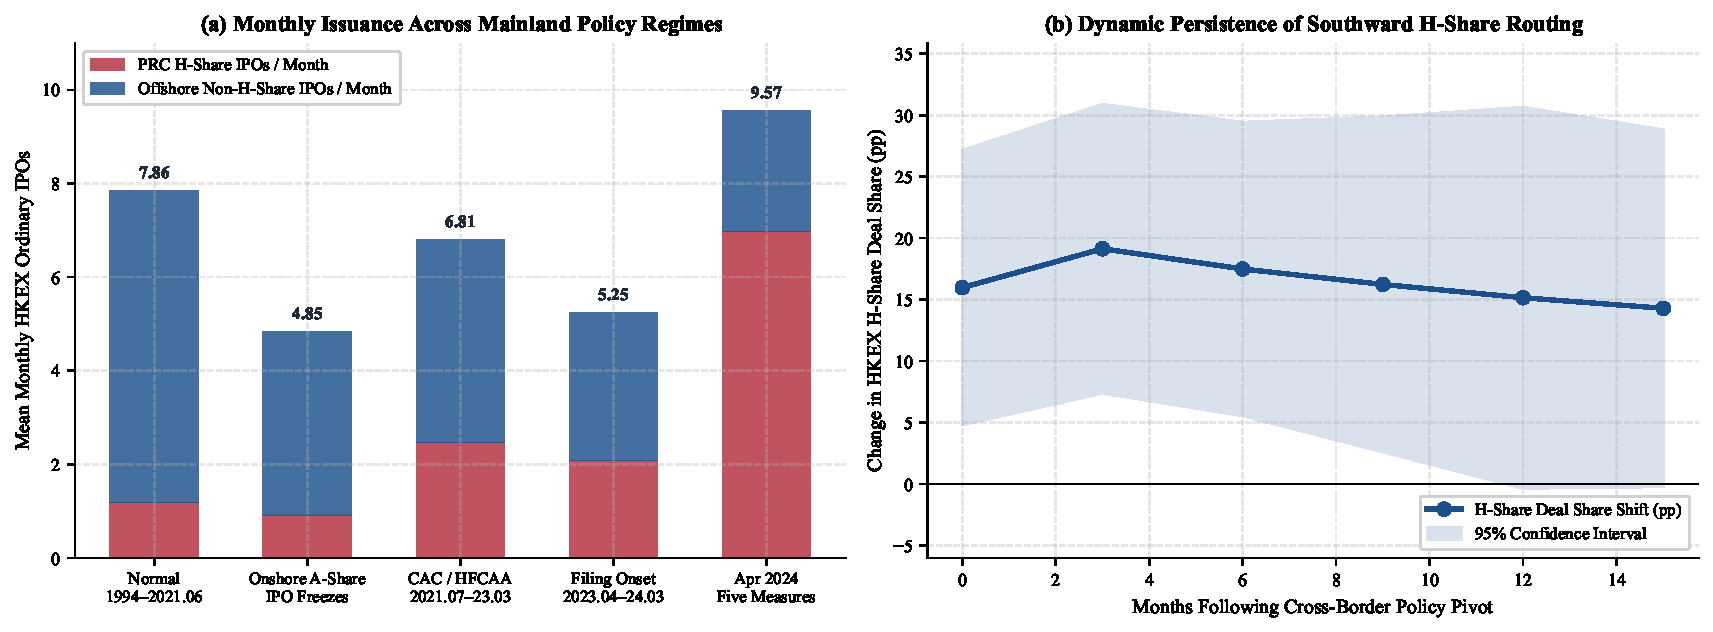
\includegraphics[width=\textwidth,height=0.80\textheight,keepaspectratio]{figures/master_fig4_1_policy_valve.pdf}
\caption*{\textbf{Figure 4.1:} Cross-border issuance across Mainland policy regimes, 1994–2026Q3 ($T = 393$ monthly observations; $N = 2,866$ ordinary IPOs on Hong Kong Exchanges and Clearing, HKEX). Panel (a) compares mean monthly People's Republic of China (PRC) H-share versus offshore non-H-share listing counts across five Mainland regulatory regimes, showing that historical A-share IPO freezes did not trigger automatic substitution (falling to \textasciitilde{}5 deals/month versus \textasciitilde{}8 in normal periods) and that southward routing surged only after the April 2024 Five Measures aligned onshore tightening with the March 2023 filing framework. Panel (b) traces the multi-month persistence of HKEX H-share deal share following major cross-border policy pivots.}
\end{figure}

The substitution channel activated forcefully only after April 2024, when three necessary conditions aligned simultaneously: onshore A-share issuance tightened persistently, the CSRC's March 2023 filing framework provided a predictable legal pathway, and Beijing explicitly endorsed Hong Kong listings by leading Mainland enterprises. Monthly HKEX issuance climbed toward ten deals, and PRC H-share issuers—historically about one deal in six—surged to roughly seven in ten offerings and four-fifths of total funds raised. The policy valve is therefore real, but conditional: it opens only when onshore rationing, a standardized cross-border legal pipeline, and a prepared cohort of seasoned issuers coincide.

Taken as a whole, Part I establishes a clear pattern of \textbf{endogenous, crisis-driven institutional evolution}: the 1973–1974 crash produced statutory supervision and the 1986 exchange merger; the 1987 B-share revolt and Black Monday closure forced the creation of the SFC, proportional voting, and paperless clearing; the 1998 market intervention yielded the Tracker Fund; the 2002 penny-stock crisis accelerated dual filing; the 2012 \textit{Hontex} fraud catalyzed Paragraph 17 sponsor accountability; losing Alibaba's 2014 IPO forced the 2018 Chapter 8A/18A/19C overhaul; GEM's shell excesses prompted the 2018–2019 anti-shell crackdown; and T+5 subscription freezes alongside post-2021 market weakness triggered FINI (2023) and Mechanism B (2025). Because historical sequencing cannot isolate individual reform effects from concurrent global liquidity cycles and Mainland policy pivots, Part II turns to micro-level mechanism tests across issuers, intermediaries, pricing rules, and aftermarket trading.

\par\vspace{16pt}\needspace{9\baselineskip}
\noindent\rule{\linewidth}{0.85pt}\par\vspace{5pt}
{\centering\Large\bfseries\color{NavyAccent} \texorpdfstring{PART II — HOW THE MARKET WORKS}{PART II — HOW THE MARKET WORKS}\par}
\vspace{4pt}\noindent\rule{\linewidth}{0.85pt}\par\vspace{8pt}
\addcontentsline{toc}{section}{\texorpdfstring{\textbf{PART II — HOW THE MARKET WORKS}}{PART II — HOW THE MARKET WORKS}}
Having traced the institutional architecture built between 1891 and 2026, Part II works through the four sets of comparisons framed in Section 1.2 (Table 1.1) in the order capital moves: from issuers, balance sheets, and gatekeeping costs (Section 5; \textit{H2}), through sponsors, syndicates, and cornerstone investors (Section 6; \textit{H2}), into bookbuilding ceilings, retail clawbacks, and margin financing (Section 7; \textit{H1}), and out into aftermarket one-year returns, lifetime wealth concentration, lockups, liquidity decay, and Stock Connect (Section 8; \textit{H3}–\textit{H4}). Five empirical regularities anchor the analysis. Most Hong Kong IPOs sell new primary shares onto corporate balance sheets rather than cashing out insiders. Direct going-public expenses exhibit steep fixed-cost scale economies, falling sharply with deal size. Mainland banks now sit on roughly nine in ten sponsor teams. Offer prices never breach the top of the published range, leaving substantial positive average first-day gains alongside a roughly one-in-three break rate. Finally, secondary-market buyers trail passive benchmarks on average over the first year, the typical listing trades well below offer in the long run, and a handful of compounding winners generate most of the aggregate gain. Throughout each section, we separate structural mechanisms verified across three decades from patterns tied to recent disclosure regimes or cyclical market heat.

\par\medskip\noindent\rule{\linewidth}{0.35pt}\par\medskip
\section*{\texorpdfstring{Section 5. Issuers: Who Lists, Who Gets the Money, and What It Costs}{Section 5. Issuers: Who Lists, Who Gets the Money, and What It Costs}}
\addcontentsline{toc}{section}{\texorpdfstring{Section 5. Issuers: Who Lists, Who Gets the Money, and What It Costs}{Section 5. Issuers: Who Lists, Who Gets the Money, and What It Costs}}
\markright{Section 5. Issuers}
Across the verified historical sample, Hong Kong IPOs serve primarily as corporate capital-raising transactions rather than insider exits: more than four in five offerings sell only new primary shares, directing about 94 cents of each gross dollar onto corporate balance sheets. Direct going-public costs exhibit steep economies of scale, falling from roughly 18\% of proceeds for the smallest issuers to about 3\% for the largest. Moreover, the initial offering rarely marks the end of public equity financing; for many listed firms, post-IPO follow-on issuance exceeds the original deal.

\subsection*{\texorpdfstring{5.1 Who Receives the Money?}{5.1 Who Receives the Money?}}
\addcontentsline{toc}{subsection}{\texorpdfstring{5.1 Who Receives the Money?}{5.1 Who Receives the Money?}}
A persistent concern surrounding offshore listings is that they operate mainly as cash-out exits for founders and pre-IPO insiders. Across the 1,862 offerings with verified share structures (1,494 on the Main Board and 368 on GEM), the evidence runs strongly the other way: pure primary offerings account for 83.5\% of verified Main Board deals (67.4\% on GEM), channeling 94.19\% of gross verified dollar proceeds directly onto corporate balance sheets. Secondary vendor sales were more common between 2000 and 2017, largely because Mainland state-enterprise privatization rules required overseas-listed SOEs to transfer shares equivalent to 10\% of IPO proceeds to the National Social Security Fund. Once that transfer mechanism was reformed in 2017 and regulatory scrutiny of pre-IPO insider sell-downs intensified, secondary tranches virtually disappeared, leaving Era V Main Board issuance almost exclusively primary (97.4\%).

Even when cash enters the corporate treasury rather than insiders' pockets, however, a natural objection remains: distressed issuers, or commercial-bank-affiliated sponsors facing lender conflicts of interest (Puri, 1996; Drucker and Puri, 2005), could still use primary equity simply to bail out existing creditors and retire troubled loans rather than to fund productive growth. If creditor bailouts or lender moral hazard drove Hong Kong issuance, prospectus use-of-proceeds disclosures should feature widespread debt retirement, commercial-bank-affiliated sponsors should systematically steer proceeds toward loan repayment, and market participants should discount offerings displaying those warning signs. Across 214 recent prospectuses with itemized allocations, the evidence weighs against a creditor-bailout channel: issuers direct proceeds predominantly toward manufacturing capacity, equipment, R\&D pipelines, overseas supply chains, and working capital, while only 18 issuers (8.4\%) earmark any proceeds for debt repayment, and commercial-bank-affiliated sponsors show little tendency to funnel equity proceeds into retiring existing bank debt. Consistent with Leone, Rock, and Willenborg (2007), moreover, primary-market investors treat debt-retirement earmarks as an adverse-selection signal over capital-allocation intent: debt-repaying issuers attract far weaker retail subscription demand (median 212.9x versus 771.9x) and lower mean Day-1 returns (+20.60\% versus +44.69\%, though the difference is not statistically significant; Table C.1). By six months post-listing, the raw buy-and-hold return differential disappears (+16.12\% versus +15.17\%), indicating that initial pricing largely absorbs the signal, although given the small 18-firm debt-repaying cell we treat the debut gap as suggestive rather than decisive. Stated allocations establish that cash entered the corporate treasury and record management's commitments, not whether capital was deployed productively; Section 10.2 examines that deployment question through matched firm trajectories.

\subsection*{\texorpdfstring{5.2 Six Doors into the Main Board}{5.2 Six Doors into the Main Board}}
\addcontentsline{toc}{subsection}{\texorpdfstring{5.2 Six Doors into the Main Board}{5.2 Six Doors into the Main Board}}
Following the 2018–2023 reforms, the Main Board ceased to operate as a single uniform gate and became a segmented architecture of six entry routes defined by issuer type, profitability, and existing public-market status (Table 5.1, Panel A). Seeing elevated post-2018 average initial returns (+18.31\%) alongside widespread cornerstone contracting (61.8\%), one might attribute both patterns to indiscriminate market sentiment across the exchange. Comparing outcomes across routes shows instead that pricing and institutional pre-commitment align sharply with observable issuer characteristics and valuation opacity (Beatty and Ritter, 1986; Rock, 1986)—while also underscoring an important caveat: because eligibility rules sort firms simultaneously by sector, scale, and financing stage, cross-route differences in Day-1 returns reflect issuer composition as well as valuation uncertainty rather than a pure effect of the listing rule itself.

At the low-opacity pole sit \textbf{already-listed dual issuers with an active onshore stock price} (A+H shares under Chapter 19A, $N = 156$), mature industrial and financial companies whose Shanghai or Shenzhen market price already anchors valuation; they raise large pools (median HK\$1,777 million) yet average just \textbf{+3.49\%} on Day 1. In the middle sit \textbf{conventional profitable companies} meeting standard profit, revenue, or cash-flow gates—either offshore holding companies (Rule 8.05, $N = 523$; median HK\$311 million; +13.07\% mean Day-1 return) or first-time Mainland-incorporated issuers without an onshore listing (non-A+H Chapter 19A H-shares, $N = 122$; +41.74\% mean)—alongside \textbf{large founder-controlled dual-class firms and overseas-listed secondary homecomings} (Chapters 8A and 19C, $N = 22$; median HK\$5,339 million; +24.65\% mean). At the high-opacity pole sit \textbf{pre-commercial biotechnology companies} eligible without revenue if a core drug candidate passes Phase I trials (Chapter 18A, $N = 95$) and \textbf{pre-commercial specialist-technology firms} in R\&D-intensive hardware, AI, and clean-tech sectors (Chapter 18C, $N = 25$); entering on unproven pipelines rather than audited profits, these issuers rely heavily on pre-committed cornerstone tranches (90.5\% and 72.0\% incidence) and exhibit the widest debut swings (+29.07\% and +59.84\%).

\begin{table}[!htbp]
\centering
\caption*{Table 5.1 — Modern Main Board Listing Tracks, Pre-IPO Ownership, and Governance (2018–2026Q3)}
\begin{adjustbox}{max width=\textwidth,max totalheight=0.79\textheight}
\begin{minipage}{\textwidth}\centering
\par\noindent{\footnotesize\bfseries Panel A: Six Statutory Main Board Gateways (2018–2026Q3, N = 943)}\par\vspace{2pt}
\footnotesize
\setlength{\tabcolsep}{3.5pt}
\renewcommand{\arraystretch}{1.18}
\begin{adjustbox}{max width=\textwidth}
\begin{tabular}{>{\raggedright\arraybackslash}p{4.03cm}cc>{\centering\arraybackslash}p{2.75cm}c>{\centering\arraybackslash}p{4.40cm}}
\toprule
Listing Track (2018–2026Q3) & Deals (N) & Med. Proceeds (HK\$M) & Cornerstone Incidence (\%) & Mean Day-1 IR (\%) & Mean 1Y BHAR vs. Hang Seng Benchmark (\%) \\
\midrule
\textbf{Rule 8.05 Offshore (Cayman / HK)} & 523 & 311 & 48.9\% & +13.07\% & -3.49\% \\
\textbf{Pure Ch. 19A PRC H-Shares (Non-A+H)} & 122 & 608 & 65.6\% & +41.74\% & -16.78\% \\
\textbf{A+H Dual-Listed Issuers} & 156 & 1,777 & 81.4\% & +3.49\% & -4.29\% \\
\textbf{Ch. 18A Pre-Revenue Biotech} & 95 & 1,260 & 90.5\% & +29.07\% & -22.14\% \\
\textbf{Ch. 18C Specialist Technology} & 25 & 981 & 72.0\% & +59.84\% & — \\
\textbf{Ch. 8A WVR / Ch. 19C Secondary} & 22 & 5,339 & 72.7\% & +24.65\% & -31.48\% \\
\textbf{All Modern Main Board} & \textbf{943} & \textbf{637} & \textbf{61.8\%} & \textbf{+18.31\%} & \textbf{-7.56\%} \\
\bottomrule
\end{tabular}
\end{adjustbox}
\par\vspace{5pt}
\par\noindent{\footnotesize\bfseries Panel B: Pre-IPO Venture Capital, State Guidance Equity, and Control Structure (2025Q1–2026Q3, N = 226)}\par\vspace{2pt}
\footnotesize
\setlength{\tabcolsep}{3.5pt}
\renewcommand{\arraystretch}{1.18}
\begin{adjustbox}{max width=\textwidth}
\begin{tabular}{>{\raggedright\arraybackslash}p{3.37cm}c>{\centering\arraybackslash}p{2.15cm}c>{\centering\arraybackslash}p{2.87cm}c>{\centering\arraybackslash}p{2.06cm}>{\centering\arraybackslash}p{2.15cm}}
\toprule
Listing Route & Deals (N) & Private VC/PE Backed (\%) & Corporate VC (\%) & PRC State / Guidance Pre-IPO (\%) & SOE Cornerstone (\%) & Med. Pre-IPO Hold (Yrs) & Med. Top-5 Customers (\%) \\
\midrule
\textbf{Ch. 18A Pre-Revenue Biotech} & 26 & 100.0\% & 75.0\% & \textbf{96.2\%} & 26.9\% & 6.9 & \textbf{94.9\%} \\
\textbf{Ch. 18C Specialist Hard-Tech} & 23 & 100.0\% & 100.0\% & \textbf{100.0\%} & 23.8\% & 8.1 & 42.3\% \\
\textbf{A+H Dual-Listed (Conventional)} & 55 & 91.3\% & 35.3\% & 28.8\% & 48.1\% & 10.2 & 41.5\% \\
\textbf{Standard Main Board (Rule 8.05 / 8A)} & 122 & 88.0\% & 64.8\% & 67.8\% & 31.1\% & 8.1 & 44.0\% \\
\textbf{All 2025–2026 IPOs} & \textbf{226} & \textbf{91.5\%} & \textbf{68.2\%} & \textbf{65.3\%} & \textbf{34.0\%} & \textbf{8.0} & \textbf{46.2\%} \\
\bottomrule
\end{tabular}
\end{adjustbox}
\end{minipage}
\end{adjustbox}
\par\vspace{3pt}\noindent\parbox{\textwidth}{\scriptsize\raggedright \textit{Notes}: Across statutory gateways, valuation opacity, institutional backing, and debut returns stratify sharply: onshore-anchored A+H dual listings show the lowest mean Day-1 return (+3.49\%) and lowest People's Republic of China (PRC) state-guidance pre-IPO equity (28.8\%), whereas pre-revenue biotechnology entrants (Chapter 18A) and pre-commercial specialist-technology entrants (Chapter 18C, the Main Board gateway for R\&D-stage hard-tech firms) carry near-universal private venture capital/private equity (VC/PE, 100\%) and PRC state-guidance backing (96.2\%–100\%), high cornerstone reliance (72.0\%–90.5\%), and the widest debut gains (+29.07\% and +59.84\%) alongside steep negative 1-year returns (-22.14\% for Chapter 18A; -31.48\% for Chapter 8A weighted voting rights [WVR] / Chapter 19C secondary listings). Reconciled modern Main Board census ($N = 943$ in Panel A, 2018–2026Q3) and closely reviewed 2025Q1–2026Q3 prospectus panel ($N = 226$ in Panel B). \textit{Day-1 IR} is initial return $(P_1 - P_0)/P_0$ from offer price $P_0$ to first-day close $P_1$; \textit{1Y BHAR vs. Hang Seng Benchmark} is one-year buy-and-hold abnormal return from $P_1$ over the estimated dividend-reinvested Hang Seng benchmark for matured listings (Chapter 18C cohorts have not yet matured to one year). In Panel B, \textit{SOE} = state-owned enterprise; backing shares use issuers with verified disclosure (private VC/PE status known for 189 of 226 issuers), while overall control across $N = 226$ is 89.4\% founder/individual/family, 6.2\% widely held, and 4.4\% directly state-asset controlled. Table 5.2 reports audited pre-IPO accounts by listing period.}
\end{table}

Pre-IPO ownership structures in the 2025–2026 cohort (Table 5.1, Panel B) clarify how Hong Kong's role in the corporate lifecycle evolved across the thirty-three-year span. Among the 189 issuers with verified pre-IPO backing status, 91.5\% carry private venture capital or private equity investment (because status is unobserved for 37 of 226 issuers, a conservative floor is at least three-quarters of all offerings), with a median pre-IPO holding period of \textbf{8.0 years} (Megginson and Weiss, 1991). That eight-year private incubation period highlights a major structural change within Hong Kong's own market. In the United States, deep private capital pools and strategic acquisitions allow many high-growth firms to stay private for a decade or more (Ewens and Farre-Mensa, 2020; Doidge, Karolyi, and Stulz, 2017). Across Greater China, by contrast, domestic markets lack an equally deep U.S.-dollar M\&A exit pool and onshore A-share queues have been periodically rationed, while dollar venture funds and finite-life renminbi guidance funds face 7-to-10-year fund-life expirations and contractual redemption (\textit{duidu}) clauses. Thus, whereas Eras I–III included younger growth listings such as Tencent (2004) alongside state privatizations, by Eras IV–V Hong Kong increasingly served as a \textbf{Year-8 hard-currency exit venue} for venture- and state-guidance-backed firms (though without private-round valuation data, completed listings alone cannot measure how much return accrued before listing; Section 8.2).

Equally distinctive is the hybrid alignment of private corporate control with state-linked pre-IPO capital. Across the 226 closely reviewed 2025–2026 issuers, 89.4\% are controlled by founders, individuals, or families and only 4.4\% are directly controlled by state-asset agencies. Yet \textbf{65.3\%} carry PRC state or municipal guidance-fund equity on the pre-IPO register—rising to \textbf{96.2\%} in Chapter 18A biotechnology and \textbf{100.0\%} in Chapter 18C specialist technology. In China's modern innovation model, private entrepreneurs retain operational control while provincial and municipal guidance funds co-finance early research and industrialization, relying on Hong Kong's public market to convert those long-duration stakes into liquid, convertible equity.

Audited pre-IPO financial statements across two decades (2005–2024; Table 5.2) confirm how those new listing channels transformed issuer fundamentals. Following our fixed financial-period rule (Appendix A.2), Year-1 is the latest audited period in each prospectus's Accountants' Report (whether a full fiscal year or a 3-to-11-month stub), Years-2 and -3 are the two complete fiscal years preceding it, and only net sales, pre-tax profit, and net profit are annualized for stub periods. Prior to 2013, virtually every Main Board issuer with verified accounts entered profitable (1.1\%–1.2\% loss-making). Following the post-2018 opening of Chapters 8A, 18A, and 18C, the Main Board loss-making share climbed to 9.2\% in 2018–2020 and jumped to \textbf{32.3\%} in 2021–2024. That shift reflects both economic design—pre-revenue biotech and hard-tech firms operate at deliberate R\&D deficits—and IFRS fair-value accounting charges on convertible preferred shares held by late-stage venture backers. That rising incidence of loss-making, late-stage venture-backed entrants pairs directly with the eight-year pre-IPO holding periods in Table 5.1: modern issuers arrive later in their valuation cycle and with heavier accounting losses than the profitable industrial and banking pioneers of the 2000s. By contrast, balance-sheet leverage remained strikingly stable across two decades, with median liabilities holding near 58\%–65\% of total assets, while median issuer scale dipped during the 2013–2017 small-cap wave (HK\$365 million in assets) before rebounding to HK\$1,458 million in 2021–2024 after minimum listing thresholds were raised. Section 8.1 examines how pre-IPO accrual quality relates to six-month post-listing returns, while Appendix C.2 reports supplementary 2025–2026 accounting comparisons on IAS 38 R\&D capitalization and thin-margin issuers near the Main Board profit threshold.

\begin{table}[!htbp]
\centering
\caption*{Table 5.2 — Audited Pre-IPO Accounts by Listing Period (2005–2024)}
\begin{adjustbox}{max width=\textwidth,max totalheight=0.79\textheight}
\begin{minipage}{\textwidth}\centering
\scriptsize
\setlength{\tabcolsep}{3.5pt}
\renewcommand{\arraystretch}{1.18}
\begin{adjustbox}{max width=\textwidth}
\begin{tabular}{lc>{\centering\arraybackslash}p{2.29cm}ccc>{\centering\arraybackslash}p{2.57cm}>{\centering\arraybackslash}p{2.38cm}>{\centering\arraybackslash}p{2.76cm}}
\toprule
Listing Period & IPOs & Usable Income Statements & Usable Balance Sheets & Med. Revenue (HK\$M) & Loss-Making, All (\%) & Loss-Making, Main Board (\%) & Med. Total Assets (HK\$M) & Med. Liabilities / Assets (\%) \\
\midrule
\textbf{2005–2007} & 203 & 94 & 67 & 920 & 1.1\% & 1.1\% & 1,523 & 65.1\% \\
\textbf{2008–2012} & 329 & 187 & 136 & 894 & 1.1\% & 1.2\% & 1,001 & 58.7\% \\
\textbf{2013–2017} & 604 & 406 & 310 & 410 & 11.1\% & 2.8\% & 365 & 57.9\% \\
\textbf{2018–2020} & 510 & 363 & 316 & 499 & 14.0\% & 9.2\% & 777 & 60.7\% \\
\textbf{2021–2024} & 309 & 234 & 229 & 936 & 32.1\% & 32.3\% & 1,458 & 61.4\% \\
\bottomrule
\end{tabular}
\end{adjustbox}
\end{minipage}
\end{adjustbox}
\par\vspace{3pt}\noindent\parbox{\textwidth}{\scriptsize\raggedright \textit{Notes}: Across cohorts, Main Board loss-making entrants jumped nearly thirtyfold after the 2018 listing-track reforms—from 1.1\%–1.2\% in 2005–2012 to 9.2\% in 2018–2020 and 32.3\% in 2021–2024—while median issuer total assets dipped to HK\$365M during the 2013–2017 small-cap wave before rebounding to HK\$1,458M after threshold hikes, and median leverage (liabilities/assets) held nearly constant at 57.9\%–65.1\%. \textit{Source}: Accountants' Reports in Hong Kong Exchanges and Clearing (HKEX) prospectuses, converted to Hong Kong dollars. Year-1 is the latest audited period, and revenue and net profit for shorter stub periods are annualized. Percentages and medians use usable statements only, so issuers whose accounts could not be confirmed are excluded rather than estimated (Appendix A.2).}
\end{table}

\subsection*{\texorpdfstring{5.3 What Does Going Public Cost?}{5.3 What Does Going Public Cost?}}
\addcontentsline{toc}{subsection}{\texorpdfstring{5.3 What Does Going Public Cost?}{5.3 What Does Going Public Cost?}}
Evaluated on explicit underwriting commissions alone, Hong Kong appears markedly less expensive than the United States, displaying none of the U.S. mid-market clustering at 7\% (Chen and Ritter, 2000; Abrahamson, Jenkinson, and Jones, 2011). Across 1,758 deals with clean fee records, underwriting spreads average 2.05\% on a proceeds-weighted basis and decline steadily with offering scale. Taken at face value, that low headline commission invites the conclusion that Hong Kong's cross-border trust architecture is nearly frictionless and equally accessible to firms of every size.

Testing whether cross-border certification instead imposes an \textbf{indivisible fixed verification cost} requires separating variable distribution fees from quasi-fixed gatekeeping outlays across offering scale (Ritter, 1987). Underwriting commissions compensate banks for scalable placement effort, whereas cross-border sponsors, multi-jurisdictional legal counsel, Big-4 reporting accountants, property and industry valuers, bilingual financial printers, and statutory filing fees represent largely fixed verification costs that must be paid whether an issuer raises HK\$300 million or HK\$30 billion. If going-public expenses were predominantly proportional, non-underwriting expense ratios would stay flat across offering scale. Decomposing the full prospectus expense schedule across proceeds quartiles refutes that proportional view (Table 5.3). Where offering scale is smallest (Q1; median proceeds HK\$400.0 million), indivisible non-underwriting legal, audit, and sponsor expenses consume 14.64\% of gross proceeds—more than four times the 3.31\% underwriting spread—pushing mean all-in direct costs to \textbf{17.95\%} (median 16.50\%; reaching 25.85\% mean below HK\$250 million). Where scale allows those fixed verification costs to amortize (Q4; median HK\$4,882.0 million), non-underwriting outlays shrink to 1.89\%, pulling total direct costs down to \textbf{3.26\%} (and below 1\% for mega-offerings such as CATL at 0.81\%). The sharp divergence between flat variable commissions and steeply regressive verification bills cleanly rules out the claim that Hong Kong's low underwriting spreads imply low entry barriers for small firms.

\begin{figure}[htbp]
\centering
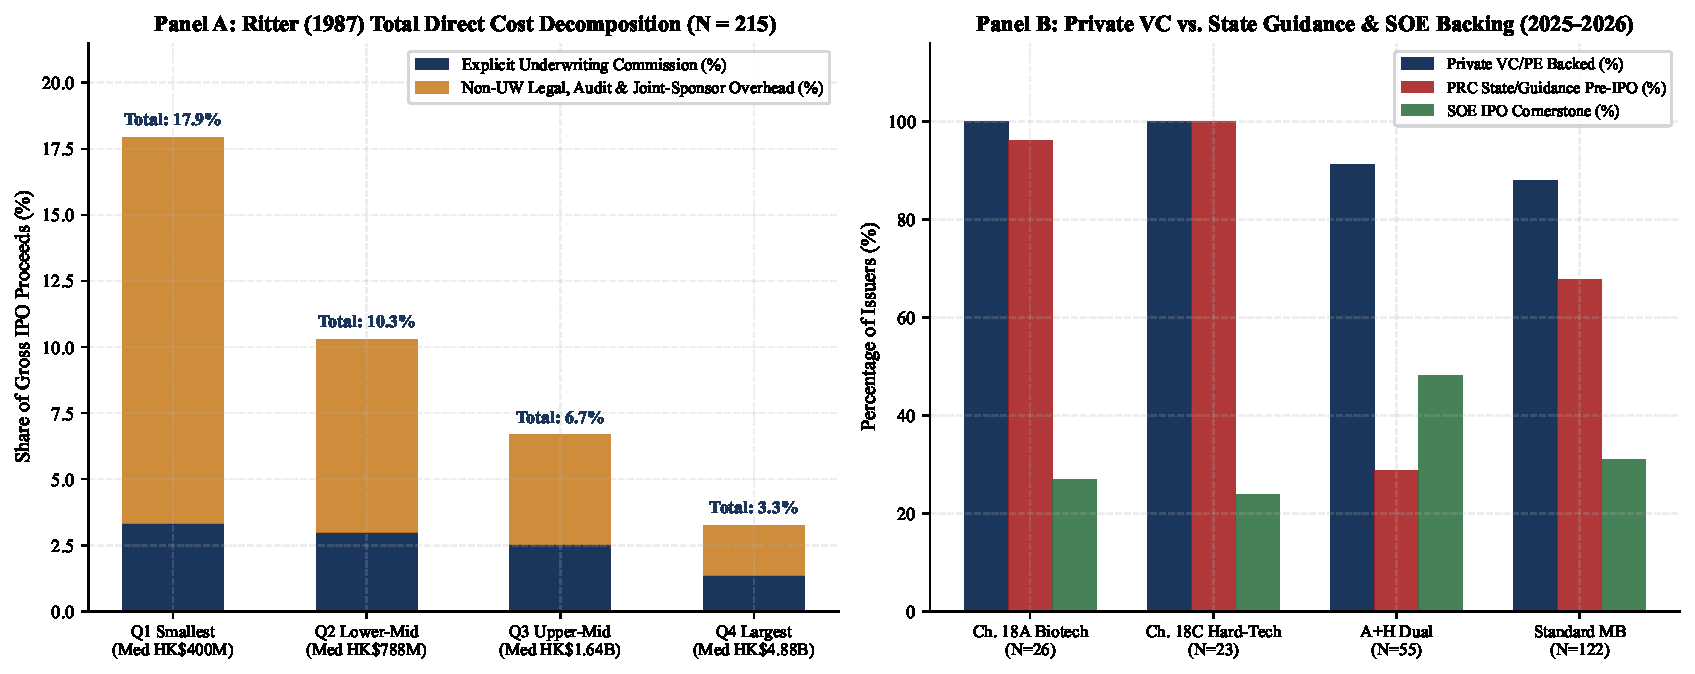
\includegraphics[width=\textwidth,height=0.80\textheight,keepaspectratio]{figures/fig10_ritter1987_total_direct_costs_and_vc_state.pdf}
\caption*{\textbf{Figure 5.1:} Direct going-public cost regressivity across deal-size quartiles and pre-IPO venture and state-guidance backing, 2025Q1–2026Q3. Panel (a) decomposes total prospectus listing expenses into explicit underwriting spreads versus non-underwriting legal, audit, and sponsor costs across Q1–Q4 gross proceeds quartiles ($N = 215$, trimming one micro-cap outlier exceeding 60\% of proceeds): mean all-in direct costs fall more than fivefold from 17.95\% in Q1 to 3.26\% in Q4 because fixed non-underwriting verification bills drop from 14.64\% to 1.89\% of proceeds. Panel (b) contrasts private venture capital/private equity (VC/PE), People's Republic of China (PRC) state/guidance fund, and state-owned enterprise (SOE) cornerstone incidence across statutory Main Board routes ($N = 226$): paired beside Panel (a), it shows which issuers clear that HK\$50M+ fixed verification floor—predominantly late-stage, institutionally incubated firms backed by VC/PE (91.5\%) and PRC state-guidance funds (65.3\%, reaching 96.2\%–100\% in pre-revenue biotech Chapter 18A and pre-commercial specialist-technology Chapter 18C), rather than unbacked small startups.}
\end{figure}

\begin{table}[!htbp]
\centering
\caption*{Table 5.3 — Direct Going-Public Cost Decomposition by Deal-Size Quartile (2025Q1–2026Q3, N = 215)}
\begin{adjustbox}{max width=\textwidth,max totalheight=0.79\textheight}
\begin{minipage}{\textwidth}\centering
\footnotesize
\setlength{\tabcolsep}{3.5pt}
\renewcommand{\arraystretch}{1.18}
\begin{adjustbox}{max width=\textwidth}
\begin{tabular}{>{\raggedright\arraybackslash}p{2.13cm}cc>{\centering\arraybackslash}p{2.41cm}c>{\centering\arraybackslash}p{3.06cm}>{\centering\arraybackslash}p{2.50cm}>{\centering\arraybackslash}p{2.50cm}}
\toprule
Gross Proceeds Quartile & Deals (N) & Med. Proceeds (HK\$M) & Med. Total Expense (HK\$M) & Explicit UW Spread (\%) & Non-UW Legal, Audit \& Sponsor (\%) & Mean All-In Direct Cost (\%) & Med. All-In Direct Cost (\%) \\
\midrule
\textbf{Q1: Smallest (\textless{} P25)} & 54 & 400.0 & 56.4 & 3.31\% & \textbf{14.64\%} & \textbf{17.95\%} & 16.50\% \\
\textbf{Q2: Lower-Mid (P25–P50)} & 54 & 787.6 & 78.2 & 2.98\% & 7.32\% & 10.30\% & 10.20\% \\
\textbf{Q3: Upper-Mid (P50–P75)} & 53 & 1,639.0 & 105.4 & 2.52\% & 4.18\% & 6.68\% & 6.55\% \\
\textbf{Q4: Largest (\textgreater{} P75)} & 54 & 4,882.0 & 169.2 & 1.37\% & 1.89\% & \textbf{3.26\%} & 2.82\% \\
\textbf{All Matched IPOs} & \textbf{215} & \textbf{1,100.0} & \textbf{89.1} & \textbf{2.55\%} & \textbf{7.02\%} & \textbf{9.56\%} & \textbf{7.97\%} \\
\bottomrule
\end{tabular}
\end{adjustbox}
\end{minipage}
\end{adjustbox}
\par\vspace{3pt}\noindent\parbox{\textwidth}{\scriptsize\raggedright \textit{Source}: 2025Q1–2026Q3 Main Board prospectus expense schedules. Of the 226 closely reviewed deals, 216 disclose both total listing expenses and percentage underwriting commissions (5 lack total listing expenses and 5 lack percentage commission rates). Table 5.3 trims one extreme micro-cap outlier exceeding 60\% of gross proceeds (Quantgroup Holding Limited, 2685.HK, whose HK\$118.4M listing bill equaled 90.52\% of its HK\$130.8M offering) so equal-weighted quartile averages ($N = 215$) are not distorted by a single small deal (retaining it lifts the equal-weighted all-deal mean from 9.56\% to 9.94\%). Section 9.2 retains all $N = 216$ complete schedules for aggregate dollar-weighted fee sums totaling HK\$24.08B on HK\$597.64B of gross proceeds (4.03\%). Across all 226 deals with usable total-expense ratios, mean total direct cost is 9.77\% and median 7.98\%, reaching 25.85\% mean / 22.08\% median below HK\$250M.}
\end{table}

The economic implication is straightforward: cross-border trust production carries a steep fixed-cost floor exceeding HK\$50 million even for the smallest Main Board entrants. The same diligence architecture that reassures international institutional investors therefore imposes a regressive entry tax on small issuers, a trade-off whose enforcement origins we trace in Section 6.4 and whose distributional consequences we weigh in Section 12.2.

\subsection*{\texorpdfstring{5.4 The IPO as the Beginning of a Financing Relationship}{5.4 The IPO as the Beginning of a Financing Relationship}}
\addcontentsline{toc}{subsection}{\texorpdfstring{5.4 The IPO as the Beginning of a Financing Relationship}{5.4 The IPO as the Beginning of a Financing Relationship}}
An initial public offering in Hong Kong is rarely a terminal capital-raising event; it inaugurates a continuing public-equity financing relationship. Across 16 of the 24 benchmark years with verified exchange statistics between 2000 and 2025, listed companies raised more equity through post-IPO placements, rights issues, and seasoned offerings than new entrants raised through IPOs (Table 5.4 and Figure 5.2). The countercyclical resilience of follow-on equity is especially pronounced during systemic downturns: in 2008, when the Global Financial Crisis shut the primary IPO window down to HK\$66.0 billion, seasoned Hong Kong issuers raised HK\$361.3 billion in follow-on equity (84.6\% of total equity raised), more than five times IPO volume; similarly, during the 2023 primary drought (HK\$46.3 billion in IPOs), follow-on issuance supplied HK\$109.7 billion (70.3\%).

\begin{table}[!htbp]
\centering
\caption*{Table 5.4 — HKEX Primary IPO vs. Post-IPO Follow-On Equity Funds Raised (Benchmark Years, 2000–2025, HK\$ Billion)}
\begin{adjustbox}{max width=\textwidth,max totalheight=0.79\textheight}
\begin{minipage}{\textwidth}\centering
\footnotesize
\setlength{\tabcolsep}{3.5pt}
\renewcommand{\arraystretch}{1.18}
\begin{adjustbox}{max width=\textwidth}
\begin{tabular}{l>{\centering\arraybackslash}p{2.24cm}>{\centering\arraybackslash}p{2.24cm}>{\centering\arraybackslash}p{2.66cm}>{\centering\arraybackslash}p{2.24cm}>{\centering\arraybackslash}p{2.01cm}>{\raggedright\arraybackslash}p{3.11cm}}
\toprule
Benchmark Year & HKEX Official IPO Funds Raised (HK\$B) & Census Ordinary IPOs (MB + GEM, HK\$B) & HKEX Post-IPO Follow-On Equity Raised (HK\$B) & Total HKEX Equity Funds Raised (HK\$B) & Post-IPO Share of Total Equity (\%) & Market Regime Context \\
\midrule
\textbf{2000} & \textasciitilde{}132.0 & 130.36 & \textasciitilde{}135.5 & \textasciitilde{}267.5 & \textasciitilde{}50.7\% & Telecom privatization \& dot-com wave (\textit{China Unicom}) \\
\textbf{2001} & 25.7 & 25.72 & \textbf{38.7} & 64.4 & \textbf{60.1\%} & Post-dot-com slump; secondary placings exceed IPOs \\
\textbf{2004} & 97.2 & 97.16 & \textbf{\textasciitilde{}179.0} & 276.2+ & \textbf{\textasciitilde{}64.8\%} & Post-SARS recovery (\textit{Tencent} IPO + heavy placings) \\
\textbf{2005} & 191.5 & 165.66 & 135.6 & 327.1 & 41.5\% & Start of SOE bank wave (\textit{BOCOM, CCB}; official incl. \textit{Link REIT}) \\
\textbf{2006} & 333.9 & 333.85 & 171.9 & 505.8 & 34.0\% & \textit{BOC} \& \textit{ICBC} mega-IPOs dominate primary total \\
\textbf{2008} & 66.0 & 65.98 & \textbf{361.3} & 427.3 & \textbf{84.6\%} & GFC freezes IPOs; balance-sheet rescues via rights/placings \\
\textbf{2009} & 248.3 & 248.23 & \textbf{393.8} & 642.1 & \textbf{61.3\%} & Post-GFC corporate \& bank equity replenishment \\
\textbf{2010} & \textasciitilde{}445.0 & 449.48 & \textasciitilde{}405.1 & \textasciitilde{}850.1 & \textasciitilde{}47.7\% & \textit{AIA} \& \textit{ABC} IPOs paired with \textit{ICBC/BOC} rights issues \\
\textbf{2014} & \textasciitilde{}227.7 & 232.33 & \textbf{\textasciitilde{}708.1} & \textasciitilde{}935.8 & \textbf{\textasciitilde{}75.7\%} & Shanghai Connect launch \& M\&A consideration shares \\
\textbf{2015} & \textasciitilde{}263.1 & 263.09 & \textbf{\textasciitilde{}848.0} & \textasciitilde{}1,111.1 & \textbf{\textasciitilde{}76.3\%} & Peak HK\$848B secondary placing/rights boom \\
\textbf{2017} & \textasciitilde{}128.2 & 128.54 & \textbf{\textasciitilde{}443.7} & \textasciitilde{}571.9 & \textbf{\textasciitilde{}77.6\%} & Secondary follow-ons outpace primary 3.5x \\
\textbf{2018} & \textasciitilde{}288.1 & 287.78 & \textasciitilde{}194.6 & \textasciitilde{}482.7 & \textasciitilde{}40.3\% & Ch. 8A/18A launch (\textit{Xiaomi, Meituan, BeiGene, Innovent}) \\
\textbf{2021} & 331.3 & 330.99 & \textbf{441.9} & 773.3 & \textbf{57.1\%} & Tech/biotech follow-on boom before mid-2021 tightening \\
\textbf{2023} & 46.3 & 46.32 & \textbf{109.7} & 156.0 & \textbf{70.3\%} & Primary drought; listed issuers tap rapid top-up placings \\
\textbf{2024} & 88.0 & 87.97 & \textbf{104.2} & 192.2 & \textbf{54.2\%} & \textit{Midea} recovery + ongoing post-IPO equity placings \\
\textbf{2025} & \textbf{285.8} & 286.89 & \textbf{358.6} & \textbf{644.4} & \textbf{55.6\%} & A+H mega-revival (\textit{CATL}) alongside surging follow-ons (\textit{Innovent}) \\
\bottomrule
\end{tabular}
\end{adjustbox}
\end{minipage}
\end{adjustbox}
\par\vspace{3pt}\noindent\parbox{\textwidth}{\scriptsize\raggedright \textit{Notes}: \textit{Measure definition}: Hong Kong Exchanges and Clearing (HKEX)'s published ``post-IPO funds raised'' series captures the exchange's \textbf{broad equity issuance total} across all listed Main Board (MB) and Growth Enterprise Market (GEM) firms rather than pure cash financing, because it combines cash-raising placements, rights issues, and open offers with non-cash consideration shares (such as M\&A share swaps, prominent in 2014–2015) and warrant/option exercises. Even with that broad definition noted, follow-on issuance exceeds primary IPO proceeds in 16 of 24 verified benchmark years and supplies a major countercyclical equity channel during primary droughts (84.6\% of total equity in 2008; 70.3\% in 2023). Abbreviations: \textit{SOE} = state-owned enterprise; \textit{GFC} = Global Financial Crisis; \textit{REIT} = real estate investment trust. \textit{Source}: HKEX \textit{Fact Books}, \textit{Annual Market Statistics}, and \textit{Annual Reports} (2002–2003 omitted where benchmark series are unverified) paired with our ordinary operating-company IPO census (Figure 5.2 plots all 24 verified benchmark years across 2000–2025).}
\end{table}

\begin{figure}[htbp]
\centering
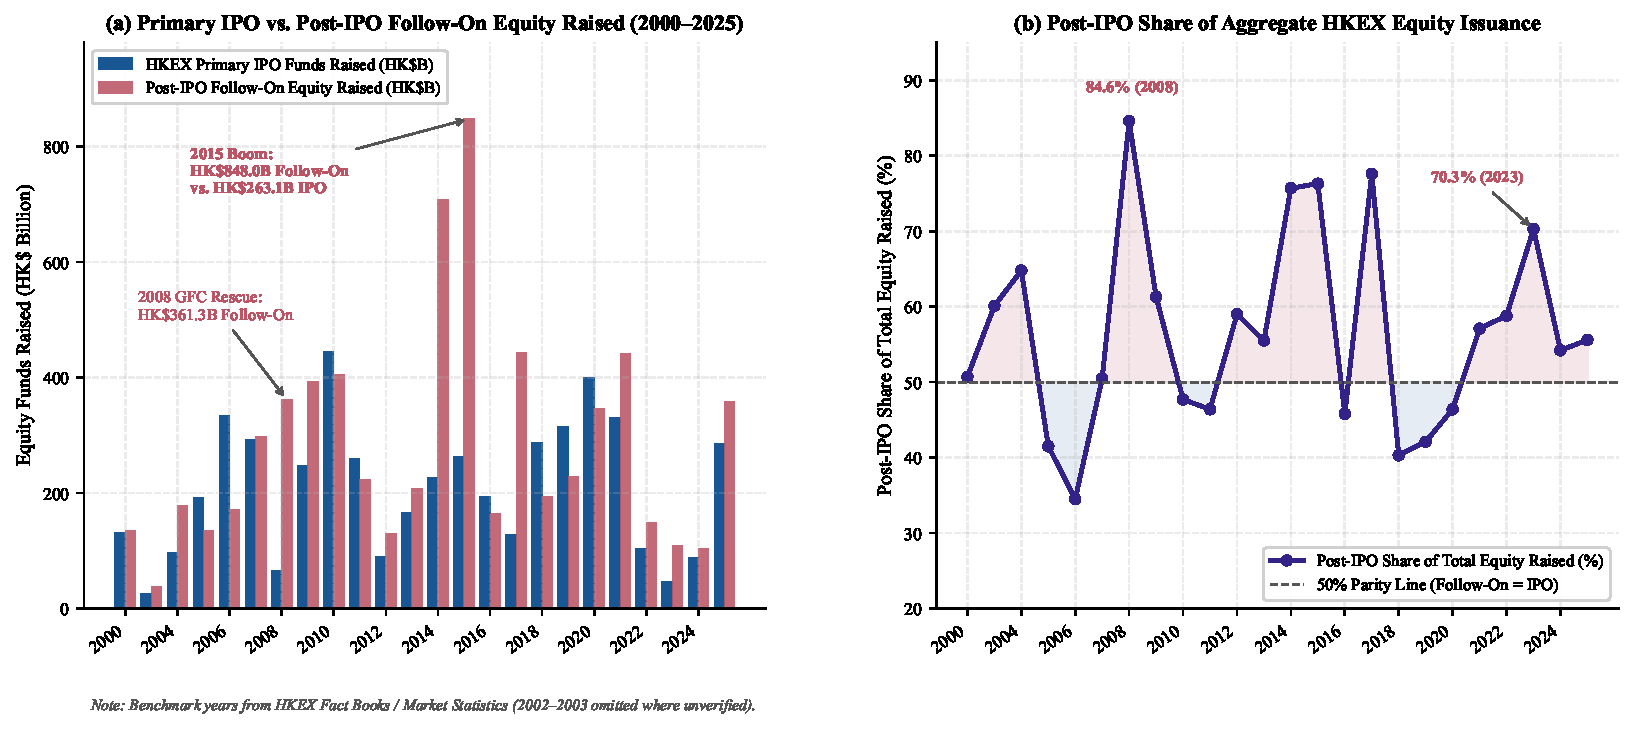
\includegraphics[width=\textwidth,height=0.80\textheight,keepaspectratio]{figures/master_fig5_2_post_ipo_lifecycle.pdf}
\caption*{\textbf{Figure 5.2:} Primary IPO versus post-IPO follow-on equity issuance on Hong Kong Exchanges and Clearing (HKEX) across 24 verified benchmark years, 2000–2025 (Main Board and Growth Enterprise Market, GEM, combined; HKEX \textit{Fact Books}). Panel (a) compares annual primary IPO proceeds against HKEX's broad post-IPO equity issuance total (HK\$B, covering cash placements, rights issues, and open offers as well as non-cash consideration shares and warrant/option exercises). Panel (b) plots the post-IPO share of total annual equity issued against the 50\% parity line, showing that follow-on issuance exceeded IPOs in 16 of 24 years and surged during primary IPO droughts (84.6\% in 2008 and 70.3\% in 2023).}
\end{figure}

Follow-on equity serves two purposes an IPO cannot. It lets existing firms repair balance sheets quickly when new listings are impossible, and it lets long-gestation firms return to investors stage by stage. Innovent is an example (Section 10.2). Tencent shows the opposite path: after its IPO it financed growth with internal cash and debt instead of public placings or rights issues.

One limit is important. The exchange totals cover all listed issuers, including long-established firms that never appear in our IPO sample, and they include some non-cash items such as consideration shares. They show that the market is a continuing source of equity, but they do not yet show how much the IPO cohorts themselves raise after listing. An issuer-level follow-on panel is the natural next step.

Several scope boundaries qualify these findings. The dominance of primary shares and the scale economies in issuance are long-run or structurally grounded facts, although share structure is verified for only part of the historical sample. The ownership, accounting, and full-cost evidence comes from 2025–2026, when the market was hot and the issuer mix was unusual. The longer history of issuer accounts in Table 5.2 starts in 2005 and covers about two-thirds of IPOs in its income-statement columns. It supports broad comparisons across periods, but the covered firms are not a random sample, and we do not use it to compare individual listing routes.

Smaller deals paid a larger share of their proceeds to list. To understand what issuers paid for, we turn to the institutions that verify, market, and distribute an offering.

\par\medskip\noindent\rule{\linewidth}{0.35pt}\par\medskip
\section*{\texorpdfstring{Section 6. Intermediaries and Enforcement: Who Vouches for the Deal?}{Section 6. Intermediaries and Enforcement: Who Vouches for the Deal?}}
\addcontentsline{toc}{section}{\texorpdfstring{Section 6. Intermediaries and Enforcement: Who Vouches for the Deal?}{Section 6. Intermediaries and Enforcement: Who Vouches for the Deal?}}
\markright{Section 6. Intermediaries and Enforcement}
Issuers paying those fixed listing bills buy verification, marketing, and distribution from a specialized group of intermediaries whose roles are strictly separated in Hong Kong. Over the past three decades, the underwriting and gatekeeping architecture of the Main Board also underwent a thorough institutional handover: where Hong Kong and British houses once led most offerings, Mainland banks now lead roughly three in four deals and appear on the sponsor team in about nine in ten, while bookrunner syndicates expanded from an average of roughly one bank to about eight and cornerstone investors grew from roughly two in five deals during 2008–2017 to three in four today. These shifts frame the central governance question of cross-border issuance: who vouches for an offering, and what happens when gatekeepers fail?

\subsection*{\texorpdfstring{6.1 Four Different Jobs}{6.1 Four Different Jobs}}
\addcontentsline{toc}{subsection}{\texorpdfstring{6.1 Four Different Jobs}{6.1 Four Different Jobs}}
A Hong Kong IPO divides work that a U.S. reader may expect to see combined under one lead underwriter. \textbf{Due-diligence gatekeepers} (\textit{sponsors}) verify the issuer's business and prospectus claims and interface directly with HKEX and the SFC. \textbf{Bookbuilding and allocation underwriters} (\textit{overall coordinators and bookrunners}) run the institutional sale and advise on final pricing and share allocation.\footnote{Under HKEX and SFC bookbuilding conduct rules effective August 2022, a sponsor-affiliated overall coordinator must generally be appointed at least two months before the listing application is filed.} \textbf{Retail distribution and margin agents} (\textit{receiving banks and retail brokers}) collect public applications and often extend subscription financing. \textbf{Financial and asset verifiers} (\textit{reporting accountants and valuers}) audit historical accounts and appraise properties or mineral assets; major international accounting firms and their predecessors worked on more than four-fifths of all IPOs in the census.

\subsection*{\texorpdfstring{6.2 From British Houses to Mainland Banks}{6.2 From British Houses to Mainland Banks}}
\addcontentsline{toc}{subsection}{\texorpdfstring{6.2 From British Houses to Mainland Banks}{6.2 From British Houses to Mainland Banks}}
Who leads Hong Kong's IPOs has changed as dramatically as who issues them. Sorting Main Board lead roles into three groups gives a clear three-act story (Table 6.1). Local and British-linked houses dominated the 1990s. Global banks rose with the large privatizations of the 2000s and peaked in Era III. Mainland institutions then took over as their clients, capital, and Hong Kong platforms grew. Since underwriter reputation is one way an issuer borrows credibility (Beatty and Ritter, 1986; Carter and Manaster, 1990), this handover also changed whose name stands behind a deal.

\begin{figure}[htbp]
\centering
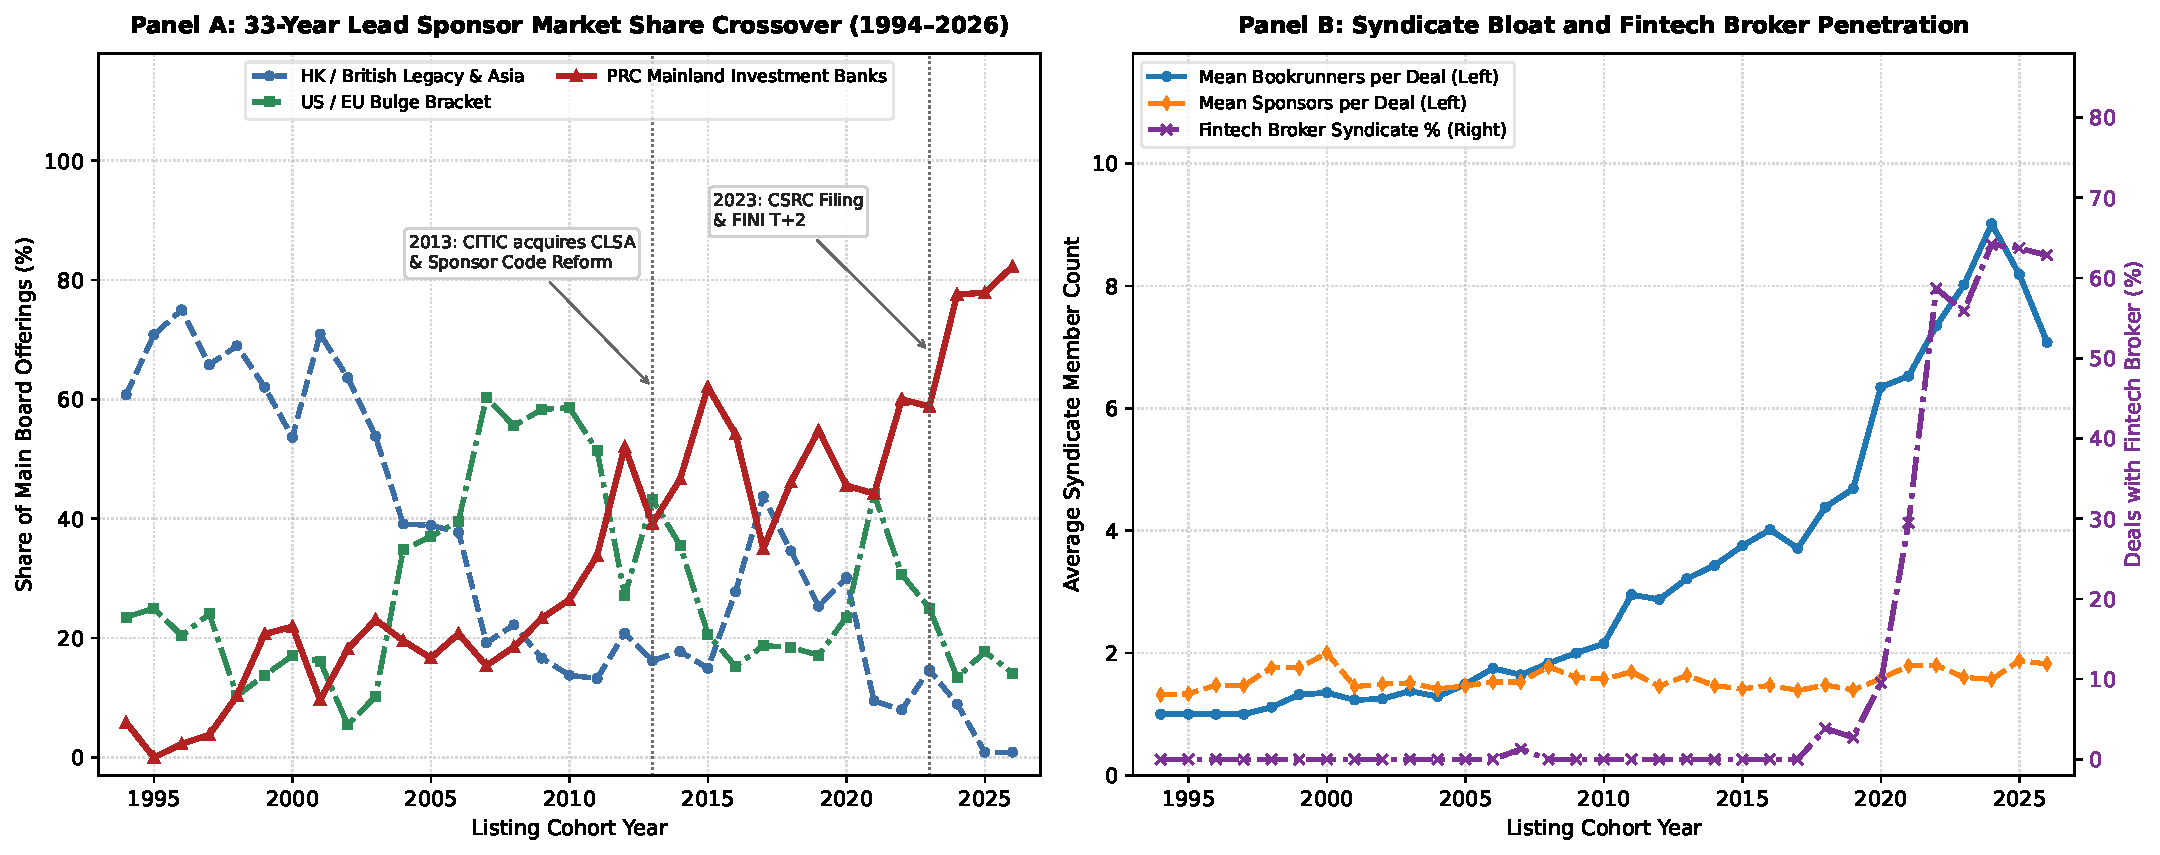
\includegraphics[width=\textwidth,height=0.80\textheight,keepaspectratio]{figures/fig11_geopolitical_ib_crossover_and_syndicate_bloat.pdf}
\caption*{\textbf{Figure 6.1:} Thirty-three-year handover in Hong Kong investment banking leadership and syndicate structure, 1994–2026Q3 ($N = 2,289$ Main Board IPO offerings). Panel (a) plots annual Main Board primary lead-sponsorship shares across Hong Kong/British legacy, U.S./European bulge-bracket, and People's Republic of China (PRC) Mainland investment banks, showing lead leadership passing from legacy houses (66.8\% in Era I) through global bulge-bracket banks (37.1\% in Era III) to PRC Mainland banks (75.6\% in Era V). Panel (b) tracks mean bookrunner counts (expanding nearly eightfold from 1.05 to 7.96), mean sponsor counts, and FinTech retail brokerage penetration (reaching 62.1\% of Era V syndicates) across the same offerings.}
\end{figure}

\begin{table}[!htbp]
\centering
\caption*{Table 6.1 — Thirty-Three-Year Main Board Syndicate Evolution, Rule 144A Retrenchment, and FinTech Distribution (N = 2,289)}
\begin{adjustbox}{max width=\textwidth,max totalheight=0.79\textheight}
\begin{minipage}{\textwidth}\centering
\scriptsize
\setlength{\tabcolsep}{3.5pt}
\renewcommand{\arraystretch}{1.18}
\begin{adjustbox}{max width=\textwidth}
\begin{tabular}{>{\raggedright\arraybackslash}p{2.13cm}c>{\centering\arraybackslash}p{1.90cm}>{\centering\arraybackslash}p{1.90cm}c>{\centering\arraybackslash}p{1.90cm}c>{\centering\arraybackslash}p{2.02cm}>{\centering\arraybackslash}p{1.90cm}c}
\toprule
Institutional Era (Main Board) & Deals (N) & HK / British Legacy Lead (\%) & U.S. / EU Bulge Lead (\%) & PRC Mainland Lead (\%) & PRC Sponsor Participation (\%) & Mean Bookrunners (N) & FinTech Broker in Syndicate (\%) & Rule 144A All / $\ge$HK\$1B (\%) & Big-4/5 Auditor (\%) \\
\midrule
\textbf{Era I (1994–1999)} & 256 & \textbf{66.8\%} & 20.7\% & 6.3\% & 12.5\% & 1.05 & 0.0\% & 0.0\% / 0.0\% & 93.4\% \\
\textbf{Era II (2000–2007)} & 397 & 43.8\% & 31.0\% & 18.1\% & 22.9\% & 1.45 & 0.3\% & 4.7\% / 12.9\% & 91.7\% \\
\textbf{Era III (2008–2017)} & 693 & 20.6\% & \textbf{37.1\%} & 40.7\% & 48.9\% & 3.14 & 0.0\% & 23.8\% / 44.3\% & 86.6\% \\
\textbf{Era IV (2018–2022)} & 582 & 23.7\% & 25.1\% & 49.7\% & 66.5\% & 5.65 & 16.2\% & 30.4\% / \textbf{62.0\%} & 85.6\% \\
\textbf{Era V (2023–2026Q3)} & 361 & \textbf{5.0\%} & \textbf{17.2\%} & \textbf{75.6\%} & \textbf{90.8\%} & \textbf{7.96} & \textbf{62.1\%} & 24.9\% / \textbf{40.8\%} & 87.5\% \\
\textbf{All Main Board} & \textbf{2,289} & \textbf{28.1\%} & \textbf{28.0\%} & \textbf{40.7\%} & \textbf{51.4\%} & \textbf{4.08} & \textbf{13.9\%} & \textbf{19.9\% / 41.1\%} & \textbf{88.1\%} \\
\bottomrule
\end{tabular}
\end{adjustbox}
\end{minipage}
\end{adjustbox}
\par\vspace{3pt}\noindent\parbox{\textwidth}{\scriptsize\raggedright \textit{Notes}: Across 33 years, primary lead leadership shifted from Hong Kong/British legacy houses (66.8\% in Era I to 5.0\% in Era V) through U.S./European bulge-bracket banks (peaking at 37.1\% in Era III) to People's Republic of China (PRC) Mainland banks (75.6\% primary lead and 90.8\% sponsor participation in Era V), while mean bookrunners expanded nearly eightfold (1.05 to 7.96), FinTech retail brokers entered 62.1\% of Era V syndicates, and Rule 144A deal incidence among HK\$1B+ offerings retreated from 62.0\% in Era IV to 40.8\% in Era V. \textit{Definitions}: 33-year Main Board syndicate census ($N = 2,289$ offerings; unit of observation is the IPO deal). Lead shares classify the primary sponsor/lead house; \textit{PRC Sponsor Participation} counts the fraction of deals with any PRC sponsor mandate; \textit{Rule 144A All / $\ge$HK\$1B} reports the \textbf{percentage of IPO deals} (not the share of stock placed) that include a Rule 144A private-placement tranche for U.S. qualified institutional buyers (QIBs)—the U.S. SEC exemption permitting offshore issuers to market shares directly to large U.S. institutions without full U.S. registration.}
\end{table}

Two related changes followed. The first concerns cross-border distribution reach. A Rule 144A tranche brings U.S. qualified institutional buyers into an offering but requires additional legal work and U.S. sales infrastructure; it became common for large IPOs in Era IV before retreating in Era V. Deals led by a U.S. or European bookrunner are far more likely to include a Rule 144A tranche (+57.3 percentage points; Table C.1), yet that association cannot be read as a causal bank-origin effect: endogenous issuer–intermediary matching means that companies actively seeking U.S. buyers hire banks equipped to reach them.

The second concerns the size and shape of syndicates. Bookrunner lists kept growing even after the 2022 conduct rules, so those rules did not end large syndicates. Meanwhile online brokers such as Futu and Tiger moved from almost nowhere to a place in most recent deals, changing how retail investors reach an IPO.

\begin{figure}[htbp]
\centering
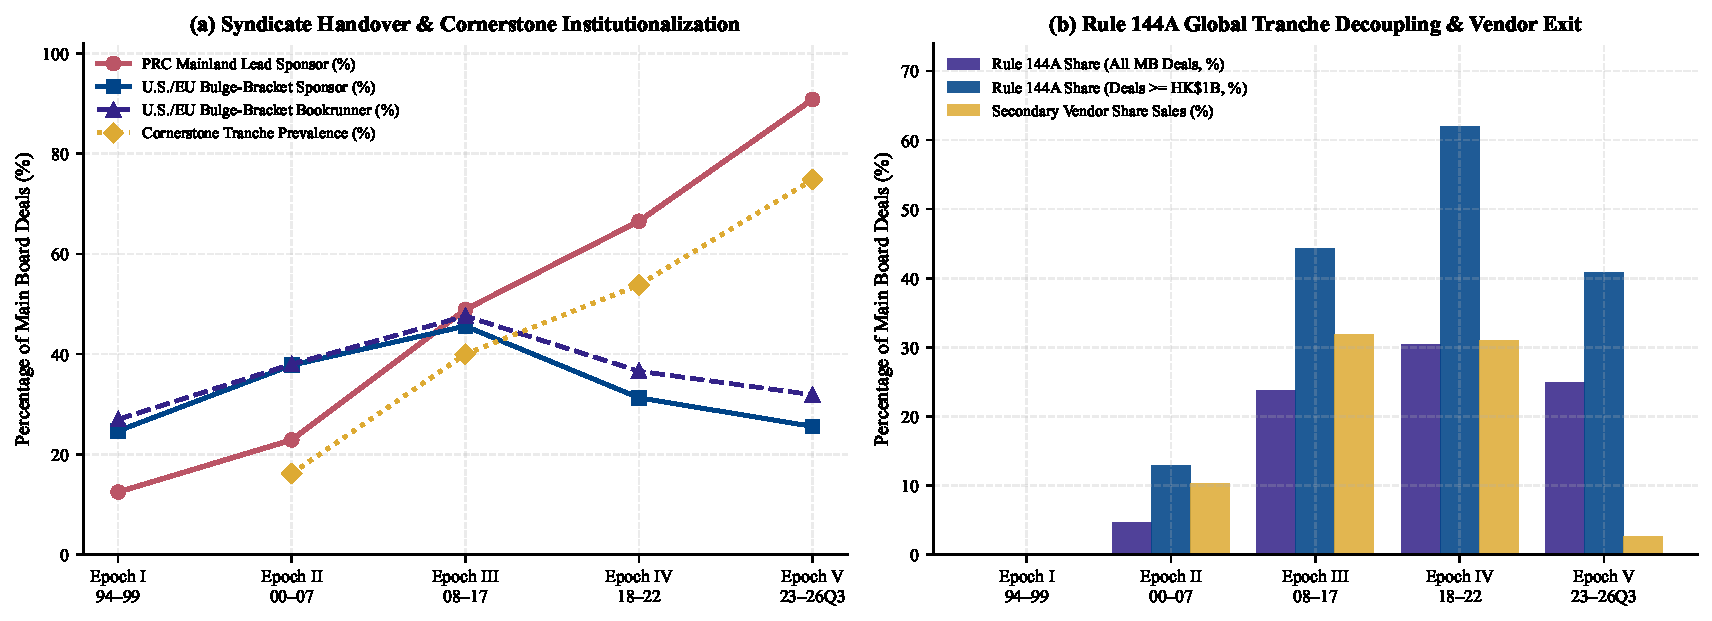
\includegraphics[width=\textwidth,height=0.80\textheight,keepaspectratio]{figures/journal_fig3.pdf}
\caption*{\textbf{Figure 6.2:} Syndicate handover, cornerstone institutionalization, and Rule 144A global tranche decoupling on the Main Board, 1994–2026Q3 ($N = 2,289$ IPO offerings). Panel (a) tracks the share of deals with People's Republic of China (PRC) versus U.S./European sponsor and bookrunner mandates alongside confirmed cornerstone tranche incidence across the five eras, showing PRC sponsor participation climbing to 90.8\% and cornerstone prevalence to 74.8\% in Era V. Panel (b) compares the \textbf{fraction of deals} carrying a Rule 144A private-placement tranche for U.S. qualified institutional buyers (QIBs, the SEC exemption for marketing offshore offerings to large U.S. institutions) across all deals and HK\$1B+ offerings against secondary vendor share sales: Rule 144A deal incidence among HK\$1B+ IPOs fell from 62.0\% in Era IV to 40.8\% in Era V as secondary vendor sales nearly vanished.}
\end{figure}

\subsection*{\texorpdfstring{6.3 Cornerstone Investors: Certification or Selection?}{6.3 Cornerstone Investors: Certification or Selection?}}
\addcontentsline{toc}{subsection}{\texorpdfstring{6.3 Cornerstone Investors: Certification or Selection?}{6.3 Cornerstone Investors: Certification or Selection?}}
Before bookbuilding closes, named cornerstone institutions commit to buy guaranteed dollar or share allocations at whatever final offer price clears the book, are disclosed in the prospectus, and accept a six-month lockup. The institution took shape during the 2005–2007 state-bank privatizations (initially contracted as ``corporate investors'' or ``corporate placings'') and was later codified in exchange guidance (HKEX-GL51-13; McGuinness, 2014). Our repaired filing series shows how far reliance on that contract has grown: among confirmed cornerstone deals on the Main Board, the conditional median tranche share of the initial pre-greenshoe offering rose from \textbf{17.0\%} in Era II (2000–2007; 16.2\% prevalence) to \textbf{28.0\%} in Era III (2008–2017), \textbf{34.6\%} in Era IV (2018–2022), and \textbf{41.4\%} in Era V (2023–2026Q3; \textbf{33.9\%} across all verified deals). Notably, as Rule 144A U.S. QIB participation in large offerings ($\ge$ HK\$1B) retreated from 62.0\% in Era IV to 40.8\% in Era V, cornerstones increasingly shifted from external prestige certification toward pre-funded, long-only anchor capacity inside an Asia-centric book.

Why did cornerstone reliance expand so dramatically, and what economic friction does the contract actually resolve? Three competing economic mechanisms could explain Table 6.2. Under an \textbf{asymmetric-information certification} channel, when sophisticated investors with reputational capital at stake, or informed insiders who already know the firm, commit locked-up capital before bookbuilding closes, their visible stake credibly signals deal quality and dampens pricing uncertainty (Beatty and Ritter, 1986; Chemmanur and Fulghieri, 1994). Under an \textbf{assured-distribution} channel, cornerstones primarily insure issuers against placement risk by pre-funding a large share of the book, a role that grew vital as Rule 144A U.S. QIB participation receded and Mainland state-linked and local-government funds stepped in. Under an unintended \textbf{float-restriction} channel, locking up 30\% to 45\% of the base offering for six months shrinks the tradable supply available to outside buyers, mechanically shaping debut volatility, the lockup calendar, and post-listing liquidity examined in Section 8 (Sections 8.3–8.4).

To probe whether cornerstone commitments operate as credible certification rather than mere placement insurance, Table 6.2 exploits cross-sectional variation in \textbf{investor information advantage and reputational capital}. If the certification story is right, pricing discipline and downside protection should be sharpest where the cornerstone possesses either private inside knowledge or repeat-market reputation to defend. Two proxies test that prediction directly. First, Panel A contrasts Chapter 18A/18C/8A offerings granted statutory waivers to bring existing pre-IPO \textbf{crossover investors} in as cornerstones—the investors with the deepest private information about pipeline quality—against peer growth issuers without crossover anchors and standard Rule 8.05/A+H offerings barred from crossover participation under Rule 10.04; crossover-backed deals post strong debut outcomes (+77.7\% mean, +103.5\% median, 14.3\% break rate), aligning with informed-insider certification, although only seven deals fall in that cell. Second, Panel B separates \textbf{global Tier-1 sovereigns and long-only managers} and \textbf{repeat hub cornerstones} ($\ge 3$ deals, carrying ongoing reputational stakes) from one-off or domestic private funds and PRC state guidance funds: offerings anchored by global Tier-1 institutions (17.8\%) or repeat hub investors (25.2\%) break issue markedly less often than those backed only by domestic private funds (35.7\%) or lacking cornerstones altogether (31.0\%).

\begin{table}[!htbp]
\centering
\caption*{Table 6.2 — Cornerstone Taxonomy Across 1,686 Placements and Network Tiers (2025Q1–2026Q3, N = 226)}
\begin{adjustbox}{max width=\textwidth,max totalheight=0.79\textheight}
\begin{minipage}{\textwidth}\centering
\scriptsize
\setlength{\tabcolsep}{3.5pt}
\renewcommand{\arraystretch}{1.18}
\begin{adjustbox}{max width=\textwidth}
\begin{tabular}{>{\raggedright\arraybackslash}p{6.20cm}ccccccccc}
\toprule
Institutional / Statutory Cornerstone Tier & Deals (N) & Mean CS Share (\%) & Mean CS Count & Med. Retail Sub (x) & Mean Day-1 IR (\%) & Med. Day-1 IR (\%) & Day-1 Break Rate (\%) & Day +180 CAR (\%) & Mean 6M BHR (\%) \\
\midrule
\rowcolor{PanelTint} \multicolumn{10}{>{\raggedright\arraybackslash}p{16.5cm}}{\textbf{Panel A: Statutory Crossover Waiver vs. Rule 10.04 Ban}} \\
Ch. 18A/18C/8A w/ Pre-IPO Crossover CS (GL92-18 / 18C.08) & 7 & \textbf{41.9\%} & 9.1 & 1,092x & +77.7\% & \textbf{+103.5\%} & \textbf{14.3\%} & -41.5\% & +12.6\% \\
Ch. 18A/18C/8A without Crossover CS & 49 & 28.9\% & 3.0 & 3,074x & +63.5\% & +28.8\% & 24.5\% & -14.1\% & +69.2\% \\
Standard Rule 8.05 \& A+H (Rule 10.04: 0\% Crossover) & 170 & 30.7\% & 5.2 & 429x & +36.1\% & +10.1\% & 28.2\% & -7.7\% & +1.5\% \\
\addlinespace[4pt]
\rowcolor{PanelTint} \multicolumn{10}{>{\raggedright\arraybackslash}p{16.5cm}}{\textbf{Panel B: Investor-Type \& Network-Centrality Taxonomy}} \\
\textbf{Global Tier-1 SWFs \& Institutions} (\textit{GIC, UBS AM, Hillhouse, Fidelity, etc.}) & 73 & \textbf{43.9\%} & 8.1 & 463x & +33.2\% & +13.3\% & \textbf{17.8\%} & -11.4\% & -5.6\% \\
\textbf{PRC State / Municipal Guidance Funds Only} (\textit{Patient Capital}) & 41 & 33.2\% & 7.0 & 551x & +36.8\% & +11.6\% & 24.4\% & \textbf{-6.3\%} & \textbf{+39.2\%} \\
\textbf{Domestic Private Corporate / Fund Cornerstones Only} & 70 & 33.9\% & 2.3 & 289x & +38.5\% & +4.4\% & 35.7\% & -11.9\% & +21.4\% \\
\textbf{Backed by Repeat Hub Cornerstones ($\ge 3$ Deals)} & 135 & 40.2\% & — & 447x & +32.9\% & +10.3\% & \textbf{25.2\%} & -7.5\% & +12.9\% \\
\textbf{One-Off / Low-Degree Cornerstones Only (1–2 Deals)} & 49 & 30.8\% & — & 301x & +44.8\% & +6.4\% & 28.6\% & -15.1\% & +26.8\% \\
\textbf{Zero Cornerstone Tranche (0\% CS)} & 42 & 0.0\% & — & 2,044x & +75.2\% & +54.2\% & 31.0\% & — & +4.2\% \\
\bottomrule
\end{tabular}
\end{adjustbox}
\end{minipage}
\end{adjustbox}
\par\vspace{3pt}\noindent\parbox{\textwidth}{\scriptsize\raggedright \textit{Notes}: \textit{Unit and sample structure}: Every row summarizes \textbf{IPO offerings} ($N = 226$ closely reviewed 2025Q1–2026Q3 Main Board deals, aggregating 1,686 individual investor-deal cornerstone placements across the 184 cornerstone-backed deals plus 42 zero-cornerstone deals). Panel A partitions all 226 offerings into three mutually exclusive statutory groups ($7 + 49 + 170 = 226$). Panel B shows two alternative, \textbf{overlapping} partitions of the same 184 cornerstone-backed offerings—first mutually exclusively by highest investor tier ($73 + 41 + 70 = 184$) and second by repeat-network centrality ($135 + 49 = 184$)—alongside the common 42 zero-cornerstone offerings ($184 + 42 = 226$). \textit{Principal contrast}: Offerings anchored by global Tier-1 sovereign wealth funds (SWFs) and long-only institutions (17.8\% break rate) or repeat hub cornerstones participating in $\ge 3$ deals (25.2\%) break issue substantially less often than deals backed only by domestic private funds (35.7\%) or lacking cornerstones (31.0\%), whereas People's Republic of China (PRC) state-fund-only deals show a higher mean 6M BHR (+39.2\%) driven by right-tail winners; formal two-stage least-squares (2SLS) weak-instrumental-variable (IV), Anderson–Rubin, and Oster (2019) bounds (Table C.1 and Appendix C.3) indicate that these differences reflect endogenous deal selection and assured distribution rather than cleanly identified causal certification. \textit{Definitions}: \textit{CS Share} is cornerstone shares divided by initial pre-greenshoe offer shares; \textit{Day-1 IR} is initial return $(P_1 - P_0)/P_0$ from offer price $P_0$ to first-day close $P_1$; \textit{Break Rate} is the share closing below offer ($P_1 < P_0$); \textit{Day +180 CAR} is cumulative abnormal return over \texttt{\small [-20,+20]} trading days around six-month lockup expiry; \textit{6M BHR} is raw six-month buy-and-hold return from $P_1$ across 161 matured issuers (to November 12, 2026); \textit{Ch. 18A / 18C / 8A} = pre-revenue biotech, pre-commercial specialist technology, and weighted voting rights routes. Repeat hub cornerstones are led by Taikang Life (32 deals), UBS Asset Management (31), Hillhouse / HHLR (29), GF Fund (29), Fullgoal (19), Perseverance (18), ICBC Wealth Management (16), Harvest (15), CICC Financial Trading (15), 3W Fund (15), Tencent (12), and GIC (12).}
\end{table}

Even after seeing lower break rates for global Tier-1 and repeat-hub cornerstones—and a 5.70 percentage-point narrower absolute first-day price dispersion ($|\text{IR}|$) across the 33-year Main Board panel ($N = 1,857$, nearly a quarter of the non-cornerstone baseline)—a skeptic should remain unconvinced that cornerstones \textit{causally} certify quality. Two competing economic channels generate the exact same pattern: \textbf{endogenous deal selection}, as sophisticated investors cherry-pick stronger or more conservatively priced deals while sponsors recruit cornerstones in anticipation of demand, and \textbf{mechanical float compression paired with Cap. 571W stabilization}, since calling $|\text{IR}|$ a ``pricing error'' treats the Day-1 close as an independent valuation benchmark even when locked cornerstone blocks shrink tradable float and stabilizing bids support the close. Formal identification tests using sponsors' pre-determined cornerstone norms, public-float thresholds, and coefficient-stability bounds confirm that none of these instruments supplies clean exogenous variation separating certification from endogenous matching (full weak-IV, Anderson–Rubin, and Oster diagnostics are reported in Table C.1 and Appendix C.3). Six-month outcomes reinforce that caution: state-fund-only deals post a higher mean return driven by a handful of winners, whereas their median is negative and close to global-institution deals. Absent data on who sells at lockup expiry, the evidence documents who anchors which deals and confirms assured distribution, without isolating a causal certification channel.

\subsection*{\texorpdfstring{6.4 What Makes the Promise Credible?}{6.4 What Makes the Promise Credible?}}
\addcontentsline{toc}{subsection}{\texorpdfstring{6.4 What Makes the Promise Credible?}{6.4 What Makes the Promise Credible?}}
Cross-border investing works only if a false prospectus has consequences even when assets sit across a border (Coffee, 2002; Siegel, 2005). Hong Kong's response developed in steps. The 2003 dual-filing arrangement gave the SFC a direct role in reviewing listing disclosure. \textit{Hontex} tested enforcement: a Mainland fabric company that listed in 2009 was found to have materially overstated its prospectus figures, and in 2012 the SFC secured a court order requiring about HK\$1 billion to be returned to public investors. Its sponsor, Mega Capital, was fined and lost its license for the relevant business.

The case led directly to reform. From October 2013, Paragraph 17 of the SFC Code of Conduct set out detailed sponsor duties, and draft Application Proofs became public early in the process. Paragraph 17 is a licensing standard enforced through regulatory sanctions. Prospectus liability itself rests in the general law, and the SFC's 2012 proposals specifically asked how that law should apply to sponsors. The practical effect was to make diligence more demanding and failure more costly. In 2018 the exchange added another tool by allowing long-suspended companies to be delisted, reducing the number of shells left in limbo.

This closes a loop with Section 5.3. Better gatekeeping is part of what makes the market acceptable to global investors. It is also part of the fixed cost that weighs most heavily on small issuers.

These institutional patterns carry clear empirical limits. The change in intermediary leadership is a 33-year fact, though classifying banks by origin involves judgment because Mainland-owned banks operate through Hong Kong entities and global banks may employ Mainland-focused teams. The cornerstone taxonomy is rich but covers only 21 months, and six-month outcomes exist for the 161 issuers that had reached that horizon by the cutoff. It supports description of who invests where, but does not identify a causal cornerstone effect. Once sponsors, syndicates, and cornerstones bring an offering to market, the next question is how Hong Kong's pricing and allocation rules divide the first-day gain.

\par\medskip\noindent\rule{\linewidth}{0.35pt}\par\medskip
\section*{\texorpdfstring{Section 7. Pricing and Allocation: Who Gets the First-Day Gain?}{Section 7. Pricing and Allocation: Who Gets the First-Day Gain?}}
\addcontentsline{toc}{section}{\texorpdfstring{Section 7. Pricing and Allocation: Who Gets the First-Day Gain?}{Section 7. Pricing and Allocation: Who Gets the First-Day Gain?}}
\markright{Section 7. Pricing and Allocation}
Across thirty-three years, Hong Kong Main Board IPOs have averaged an initial return of about 14\%, yet the median offering gains only about 2.5\% and roughly one in three finishes below its offer price. Not one of nearly two thousand offerings with an indicative price range priced above the top of that range. Aggregated over the full sample, the gap between first-day closing prices and offer prices represents more than HK\$600 billion left on the table. Who captures that surplus depends on how shares are allocated, how retail applications are financed, and how far subscription demand exceeds supply.

\subsection*{\texorpdfstring{7.1 Why the Top of the Range Binds}{7.1 Why the Top of the Range Binds}}
\addcontentsline{toc}{subsection}{\texorpdfstring{7.1 Why the Top of the Range Binds}{7.1 Why the Top of the Range Binds}}
A Hong Kong Main Board IPO follows a fixed four-stage sequence: \textbf{publication of an indicative price range} in the prospectus, \textbf{concurrent retail public subscription and institutional bookbuilding}, \textbf{final offer-price determination and share allotment}, and \textbf{first-day exchange trading}. In a U.S. bookbuild, strong institutional demand routinely pushes the final offer price \textbf{above the top of the filing range} (distinct from simply pricing above the range midpoint), rewarding bidders who reveal positive valuation information (Benveniste and Spindt, 1989; Hanley, 1993; Cornelli and Goldreich, 2001). Hong Kong inverted that mechanism because retail applicants subscribe simultaneously at the \textbf{top of the published offer range}, so raising that ceiling mid-offer would invalidate submitted public applications and require cancelling or re-soliciting the offering.\footnote{Historically, retail subscribers submitted physical white or yellow application forms at receiving-bank branches accompanied by cashier orders or cheques funded at $P_{\max}$ plus statutory brokerage and transaction levies, with unallotted funds refunded after allotment.} Even after electronic settlement eliminated paper applications, the \textbf{statutory hard ceiling} remained in place as a retail-protection rule. Across all 1,943 HKEX deals with a classified price range (1,702 Main Board and 241 GEM), not a single offering priced above the top of the published offer range. A small number priced below the range, and they performed poorly.

Observing zero offerings priced above the top of the published offer range alone does not prove that the statutory ceiling constrains price discovery. Pricing above the top of the range requires cancelling the offer and relaunching with a supplemental or new prospectus, HKEX declined to introduce an upward flexibility mechanism in 2025, and an offer that would have needed one may simply never complete. Zero breaches are therefore also compatible with wide initial ranges and with selection on completed deals.

To ask whether the ceiling binds in a way that moves value into Day-1 trading, we follow how Hang Seng price index news passes into prices (Hanley, 1993), and we split the offer window at the recorded pricing date. News that arrives before pricing can move both the offer price $P_0$ and the debut price $P_1$; news that arrives after pricing can move only $P_1$. If the ceiling binds, good news before pricing cannot push $P_0$ above the top of the published offer range and should therefore show up as a higher first-day return from the offer price. An earlier version of this analysis measured the window from the prospectus date to the day before listing, which mixed the two kinds of news. On the full window, a falling market passes into first-day returns from the offer price (slope +1.49) and a rising market does not (-0.08). Splitting the window for the 1,727 Main Board offerings with a usable pricing date locates that asymmetry \textit{before} pricing: a 5\% drop in the index between launch and pricing lowers the first-day return by about 11 percentage points (slope +2.24, $t = 3.36$), whereas a rise of the same size is associated with a slightly \textit{lower} first-day return (-1.43, $t = -2.78$). News after pricing passes through at about 0.7 in both directions and is not statistically distinguishable from zero. Offer prices do respond to falling markets, but only a little: within the range, a 5\% pre-pricing drop in the index lowers the final offer price relative to the top of the published offer range by about 2.7\%, and a 5\% rise does not move it measurably (Appendix C.3).

These patterns do not support the reading that the ceiling pushes positive news into debut gains. They fit an offer price that adjusts only partly to bad news before pricing, consistent with the partial adjustment documented by Hanley (1993) and Loughran and Ritter (2002), here concentrated on the downside. Fixed-price offerings, which cannot adjust at all, show larger pass-through in both directions, but there are only 134 of them in the split sample and many priced at launch, so we do not lean on that comparison.

\begin{table}[!htbp]
\centering
\caption*{Table 7.1 — Comparative Primary Pricing \& Allocation Architecture: Hong Kong, United States, and Mainland A-Shares}
\begin{adjustbox}{max width=\textwidth,max totalheight=0.79\textheight}
\begin{minipage}{\textwidth}\centering
\footnotesize
\setlength{\tabcolsep}{3.5pt}
\renewcommand{\arraystretch}{1.18}
\begin{adjustbox}{max width=\textwidth}
\begin{tabular}{>{\raggedright\arraybackslash}p{2.90cm}>{\raggedright\arraybackslash}p{4.30cm}>{\raggedright\arraybackslash}p{4.30cm}>{\raggedright\arraybackslash}p{4.30cm}}
\toprule
Institutional Feature & Hong Kong (HKEX Main Board) & United States (NYSE / Nasdaq) & Mainland China (SSE / SZSE A-Shares) \\
\midrule
\textbf{Retail / Institutional Timeline} & Simultaneous public prospectus + institutional bookbuilding & Institutional bookbuilding first; retail receives post-pricing allocations & Separate online retail lottery (\textit{wangshang}) + offline institutional allotment (\textit{wangxia}) \\
\textbf{Pricing Above Top of Offer Range} & \textbf{0.0\%} (0 / 1,943 range deals; statutory hard ceiling) & \textbf{21.4\%} of operating IPOs price above top of filing range & Historically capped by \textbf{23x P/E ceiling} (pre-registration reform) \\
\textbf{Minimum / Mandatory Retail Tranche} & Legacy \textbf{PN18} (10\% $\to$ 50\% clawback); \textbf{Aug 2025 Mech. B} ($\ge 10\%$ initially, 0\% mandatory clawback) & No statutory retail tranche; discretionary broker distribution & High statutory retail lottery allocation with 100\% pre-settlement/post-lottery rules \\
\textbf{Pre-IPO Cornerstone Lockups} & \textbf{74.8\%} of Era V deals (median \textbf{41.4\%} of base offer; 6M lockup) & Rare; informal anchor indications without statutory 6M lockup & Strategic placement (\textit{zhanlue peishou}) with 12M+ lockup on large STAR/ChiNext deals \\
\textbf{Settlement \& Margin Mechanics} & \textbf{FINI T+2} credit-cap confirmation (Nov 2023; 90\% retail margin) & T+1 / T+2 DVP institutional settlement; no retail lottery margin & Pre-allocated market-value quota (\textit{shizhi peishou}); cash paid upon winning \\
\textbf{Price Stabilization} & \textbf{Cap. 571W} (30-day greenshoe up to 15\% + stabilizing bids at $\le P_0$) & SEC \textbf{Reg M} (30-day 15\% greenshoe + syndicate short covering) & Restricted; 30-day greenshoe permitted only on select mega-IPOs \\
\bottomrule
\end{tabular}
\end{adjustbox}
\end{minipage}
\end{adjustbox}
\par\vspace{3pt}\noindent\parbox{\textwidth}{\scriptsize\raggedright \textit{Notes}: \textit{Why Hong Kong is informative}: Unlike the United States (where institutional bookbuilding precedes discretionary retail allocation and 21.4\% of IPOs price above the top of the filing range) or Mainland A-shares (historically capped by P/E ceilings and separate lotteries), Hong Kong Exchanges and Clearing (HKEX) is the only major market pairing simultaneous public/institutional bookbuilding with a \textbf{binding statutory price ceiling} at the top of the published offer range (never breached across 1,943 range deals), codified mechanical retail clawbacks (legacy Practice Note 18 [PN18], superseded in August 2025 by Mechanism B setting an initial public subscription share of at least 10\% with no mandatory clawback), statutory 6-month cornerstone lockups (74.8\% of Era V deals), and exact published ballot schedules settled via Fast Interface for New Issuance (FINI, T+2 credit-cap confirmation). Abbreviations: \textit{NYSE / Nasdaq} = New York Stock Exchange / Nasdaq; \textit{SSE / SZSE} = Shanghai / Shenzhen Stock Exchanges; \textit{SEC Reg M} = U.S. Securities and Exchange Commission Regulation M; \textit{DVP} = delivery versus payment; \textit{Cap. 571W} = Hong Kong Securities and Futures (Price Stabilizing) Rules. \textit{Source}: Institutional synthesis from HKEX Listing Rules, SEC Regulation M, Qian, Ritter, and Shao (2024), and the census ($N = 2,866$).}
\end{table}

Yet a further puzzle arises from Era V's headline distribution: how can the exact same offer-range rulebook simultaneously generate a striking mean first-day return from the offer price (\textbf{+29.59\%}; \textbf{+53.15\%} in 2026Q1–Q3), a modest median (\textbf{+5.00\%}), and a \textbf{31.1\%} break rate (Table 4.1)? If ceiling-induced mispricing is driven by \textbf{unanchored valuation uncertainty colliding with restricted tradable float and leveraged retail demand}, then explosive debut pops should vanish wherever an external market price already anchors valuation, and concentrate precisely where tradable supply is tightest. Separating Era V offerings by the presence of an active cross-market price anchor resolves the bimodal puzzle cleanly. Where liquid onshore A-share quotes anchor pricing directly, among \textbf{A+H dual-listed issuers}, valuation disagreement is bounded and first-day returns from the offer price average a modest \textbf{+3.49\%} (Table 5.1, Panel A), pulling down the cross-sectional median. Where no public price anchor exists (Pure Chapter 19A H-shares at +41.74\% mean, Chapter 18A biotechs at +29.07\%, and Chapter 18C specialist-technology listings at +59.84\%), \textbf{41.4\%} median six-month cornerstone lockups (Section 6.3), Mechanism B's \textbf{initial public subscription tranche of at least 10\% with no mandatory oversubscription clawback}, the statutory ceiling at the top of the published offer range, and \textbf{62.1\%} FinTech retail brokerage penetration (Table 6.1) leave leveraged online retail demand chasing a compressed unrestricted Day-1 float, generating an extreme right tail without insulating weak issues from breaking offer.

\subsection*{\texorpdfstring{7.2 Retail Clawback and the 2025 Reform}{7.2 Retail Clawback and the 2025 Reform}}
\addcontentsline{toc}{subsection}{\texorpdfstring{7.2 Retail Clawback and the 2025 Reform}{7.2 Retail Clawback and the 2025 Reform}}
For 27 years, Practice Note 18 (1998) paired that hard price ceiling with an automatic supply transfer from institutions to retail applicants triggered by the \textbf{public oversubscription multiple}—defined as public shares applied for divided by the initial pre-clawback public offer shares (typically 10\% of the base offering). Crossing the first statutory trigger at \textbf{15x} expanded the retail share from 10\% to 30\%, with further mandatory steps at higher demand tiers up to 50\% (Vong and Trigueiros, 2017).\footnote{Under legacy Practice Note 18 (1998–July 2025), the standard 10\% initial public offer tranche stepped up automatically to 30\% when retail oversubscription reached 15x–50x, 40\% at 50x–100x, and 50\% at 100x or above.} Just above the 15-fold subscription threshold, the retail share of the offer was about 20 percentage points higher, and the ratio of the first-day closing price to the offer price was about 22\% lower (Figure 7.1a, for IPOs near the 15-fold subscription threshold). That drop poses an immediate economic puzzle: does shifting marginal supply into short-horizon retail hands genuinely absorb secondary-market buying pressure, or do issuers crossing 15x simply price higher at the offer or sort endogenously around the cutoff? Both the offer price ($P_0$) and where the final offer price falls within the range are flat across the threshold once deal scale is accounted for, so the lower debut ratio is not explained by higher offer prices above 15x. Two features keep us from reading it causally. Pre-determined issuer characteristics shift near the 15-fold subscription threshold: the share of PRC H-share issuers falls by 18.5 percentage points, and deal proceeds and cornerstone backing also differ nearby. And the subsample of “non-waiver” contracts, where the drop is larger (-0.372 log points), is chosen by whether the final allocation matched the PN18 schedule, which is itself an outcome of the clawback; it is not a clean test of waivers (full bandwidths, price-level decompositions, and balance diagnostics are documented in Table C.1 and Appendix C.3). The 15x evidence is therefore consistent with marginal retail supply dampening debut gains, but it is an association, not a quasi-experimental estimate. At extreme subscription levels (100x+), both the top of the published offer range and the 50\% clawback cap bind simultaneously, leaving excess demand to clear entirely on Day 1 (Derrien, 2005; Ljungqvist, Nanda, and Singh, 2006).

\begin{figure}[htbp]
\centering
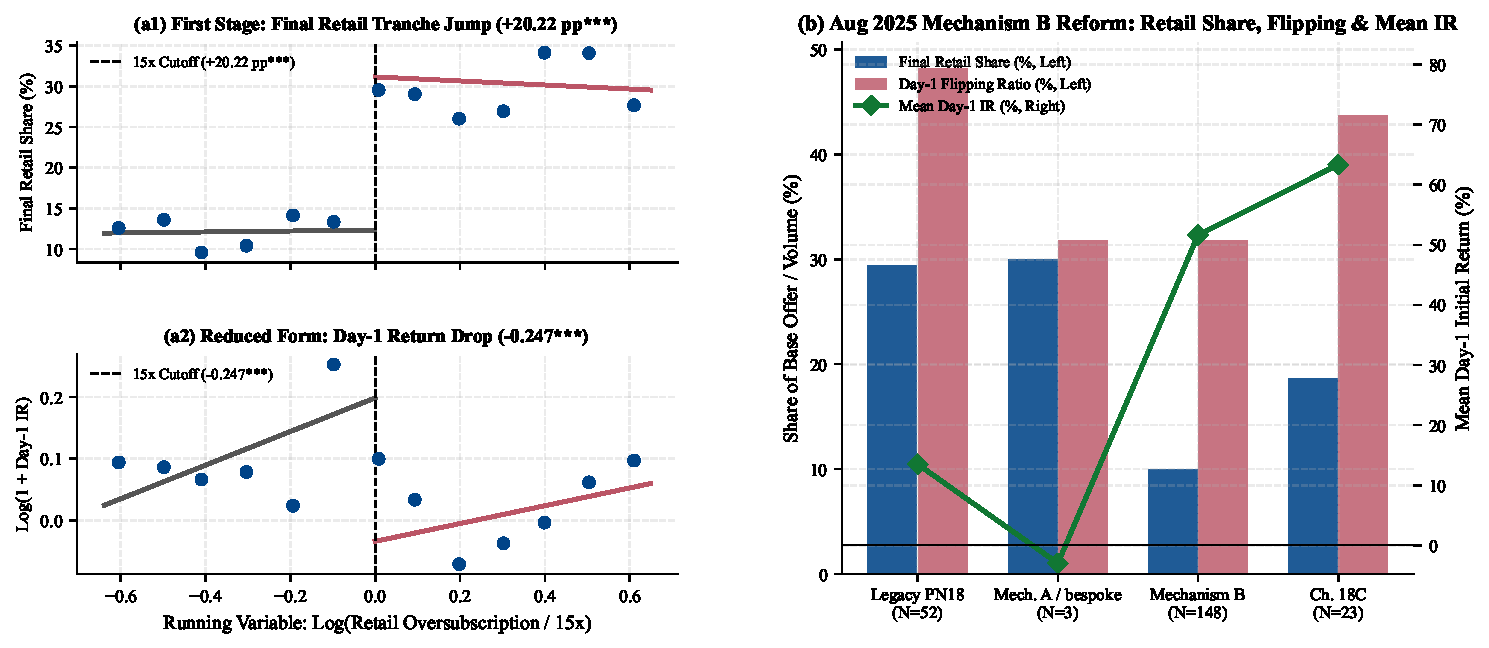
\includegraphics[width=\textwidth,height=0.80\textheight,keepaspectratio]{figures/journal_fig6.pdf}
\caption*{\textbf{Figure 7.1:} Mandatory retail clawback threshold jumps and the August 2025 Mechanism B allocation overhaul. \textit{Note on samples}: the two samples marked $N = 226$ refer to \textbf{different comparisons}. Stacked left panels examine $N = 226$ historical Main Board IPOs (1998–July 2025) near the Practice Note 18 (PN18) 15-fold retail oversubscription trigger (bandwidth $|z| \le 0.45$, 114 below and 112 above)—where the oversubscription multiple is public retail shares applied for divided by initial pre-clawback retail offer shares, and the running variable is $z = \log(\text{retail oversubscription multiple} / 15)$—showing (a1) a +20.22 pp jump in final retail tranche share ($t = 5.07$) and (a2) a -0.247 log-point drop (about 22\% lower) in the ratio of the first-day closing price to the offer price, $\log(P_1/P_0)$ ($t = -3.08$). Right panel (b) examines a \textbf{separate} sample of $N = 226$ closely reviewed 2025Q1–2026Q3 Main Board offerings across Legacy PN18 (mandatory clawback up to 50\%, $N = 52$), post-August 2025 Mechanism A / bespoke step-up clawback ($N = 3$: two statutory Mechanism A deals plus one bespoke waiver), post-August 2025 Mechanism B (initial public subscription share of at least 10\%—up to 60\%—with no mandatory oversubscription clawback, chosen by 98.0\% of eligible non-18C post-reform issuers once allocation mechanisms are verified against the prospectus text, $N = 148$), and Chapter 18C (pre-commercial specialist technology, capped 5\%$\to$20\% clawback, $N = 23$): moving from Legacy PN18 to Mechanism B cuts mean final retail allocation from 29.4\% to 10.0\% (before-and-after shift -19.30 pp with prospectus-time controls) and lowers mean first-day trading volume relative to shares offered from 48.2\% to 34.7\% (before-and-after -9.98 pp, $p = 0.007$), while mean first-day returns from the offer price rise from +13.51\% to +51.63\% alongside hotter market conditions (+63.35\% in Chapter 18C).}
\end{figure}

The \textbf{August 2025 reform}, which applies to listing documents published on or after August 4, 2025 (HKEX, 2025), replaced mandatory Practice Note 18 clawbacks with an issuer choice between two allocation tracks while simultaneously introducing a \textbf{40\% minimum institutional bookbuilding tranche} and revised \textbf{initial public-float requirements}. Under \textbf{Mechanism A}, issuers keep a step-up retail clawback schedule;\footnote{Under August 2025 Mechanism A (Practice Note 18 Paragraph 4.2(a)), the initial public offer tranche starts at 5\% and steps up to 15\% at 15x–50x, 25\% at 50x–100x, and 35\% at 100x or above. WeRide (0800.HK) received a bespoke waiver stepping from 5\% initially to 10\% at 10x and 20\% at 50x.} under \textbf{Mechanism B}, issuers set an \textbf{initial public subscription share of at least 10\% (up to 60\%) with no mandatory oversubscription clawback}, though limited discretionary reallocation remains permitted. Our first classification inferred Mechanism A whenever the final public share exceeded 14\%; that rule is incompatible with permissible Mechanism B reallocations, and six 2026 issuers labelled A in fact state Mechanism B in their prospectuses (1609, 7630, 2553, 6067, 6228, and 1191), whereas only two statutory Mechanism A issuers (2631 and 2580) explicitly invoke the step-up clawback schedule in their prospectuses. WeRide (0800) used a waiver-based bespoke schedule and is kept apart from statutory Mechanism A, as are the 23 Chapter 18C listings governed by Rule 18C.09. After these corrections, \textbf{98.0\% (148 of 151)} of eligible non-18C issuers chose Mechanism B. Because only two statutory Mechanism A deals (plus one bespoke waiver) appear in the updated panel, the data cannot support a direct comparison of Mechanism A against Mechanism B, and instead provide a before-and-after contrast around the August 2025 package as a whole.

If eliminating mandatory retail clawbacks keeps shares in longer-horizon institutional hands and tightens unrestricted Day-1 float, then post-reform offerings should exhibit smaller retail pools, quieter debut trading, and sharper upward price pressure where float compression binds tightest. At first glance, high-demand ($\ge 100\times$) offerings after August 2025 fit that script dramatically: final retail share drops by \textbf{16.0 percentage points} and \textbf{first-day trading volume relative to shares offered} falls by \textbf{20.3 percentage points} (Figure 7.1b). Yet two economic objections prevent equating that conditional drop with a causal decline in ``flipping'' (actual resales by allotted investors). First, exchange-level trading volume captures repeated intraday trades by non-allottees rather than verified resales by original retail recipients (Aggarwal, 2003). Second, conditioning on $\ge 100\times$ oversubscription is mechanically tainted by a post-reform rule change: because Mechanism B keeps the initial retail pool small, identical dollar demand automatically generates a higher oversubscription multiple (lifting the share of deals crossing $100\times$ from 55.8\% to 82.2\%), while the mechanism is chosen by the issuer. Running the \textbf{before-and-after comparison} across all 226 offerings, with the regime assigned by prospectus date and only controls fixed when the prospectus is published (maximum offer size, A+H status, Chapter 18A and 18C status, and sector), removes the conditioning on demand. After August 2025, final retail allocations are \textbf{19.3 percentage points} lower (about two-thirds of the pre-reform mean of 29.4\%) and first-day trading volume relative to shares offered is \textbf{10.0 percentage points} lower ($p = 0.007$; about a fifth of the pre-reform mean), while the first-day closing price relative to the offer price is higher (+0.190 log points). An earlier specification that also controlled for realized proceeds and cornerstone shares, both fixed only at pricing, gives similar figures (-18.8 and -8.5 percentage points; Appendix C.3). This is a before-and-after comparison, not an intention-to-treat estimate: every issuer after the reform faced the new bookbuilding-tranche and free-float rules along with the choice of mechanism, and the post-reform months coincided with a strong market. The reform clearly reduced the retail share of new issues; how much of the lower first-day trading volume comes from Mechanism B itself remains open.

\subsection*{\texorpdfstring{7.3 Financing the Queue: Margin, HIBOR, and FINI}{7.3 Financing the Queue: Margin, HIBOR, and FINI}}
\addcontentsline{toc}{subsection}{\texorpdfstring{7.3 Financing the Queue: Margin, HIBOR, and FINI}{7.3 Financing the Queue: Margin, HIBOR, and FINI}}
Retail participation in Hong Kong is cheap to enter and easy to lever. A single board lot in 2026 typically costs a few thousand Hong Kong dollars (median ticket HK\$4,358), and online brokers extend high-leverage margin financing for larger applications; early margin demand predicts final subscription, consistent with informational cascades (Welch, 1992). For decades, prefunding those applications linked primary equity issuance directly to Hong Kong's currency board (Section 2.1). During landmark mega-offerings—most visibly ICBC in 2006, AIA in 2010, Ant Group's suspended subscription wave in 2020, and CATL's A+H revival in 2025—surging cross-border inflows prompted automatic HKMA foreign-exchange interventions that expanded the banking system's \textbf{Aggregate Balance} (the sum of commercial banks' clearing-account balances held at the HKMA, which anchors domestic interbank liquidity), even as pre-allotment cash lockups temporarily tightened short-term interbank funding rates (HIBOR).\footnote{When cross-border IPO inflows push the Hong Kong dollar against the HK\$7.75 strong-side Convertibility Undertaking, the Hong Kong Monetary Authority automatically buys U.S. dollars and sells Hong Kong dollars, increasing the Aggregate Balance.} When FINI launched in November 2023, it compressed the average prospectus-to-listing interval from roughly two weeks to nine days (and pricing-to-listing from seven days to four) while replacing full cash prefunding with targeted bank credit confirmations.

Over the full 1999–2026 history, allotment-week 1-week HIBOR shifts ease by nearly 40 basis points (bp) after FINI (Table C.1), and post-FINI mega-subscriptions exhibit calmer short-term funding spreads (Figure 7.2a). Even so, a quarter-century comparison risks confounding settlement modernization with shifting global interest-rate cycles and Hong Kong's Aggregate Balance. Isolating \textbf{mega-subscription waves ($\ge$ HK\$100B)} within the single comparable \textbf{2021–2026 monetary regime}—where removing cash-lockup friction should bite hardest—yields no statistically distinguishable HIBOR break because few mega-offerings arrived during the quiet pre-FINI window while global policy rates moved concurrently (detailed specification in Appendix C.3). FINI thus verifiably compressed settlement timelines and dismantled mechanical prefunding lockups, even though its isolated money-market rate impact cannot be separated from macro rate cycles.

\begin{figure}[htbp]
\centering
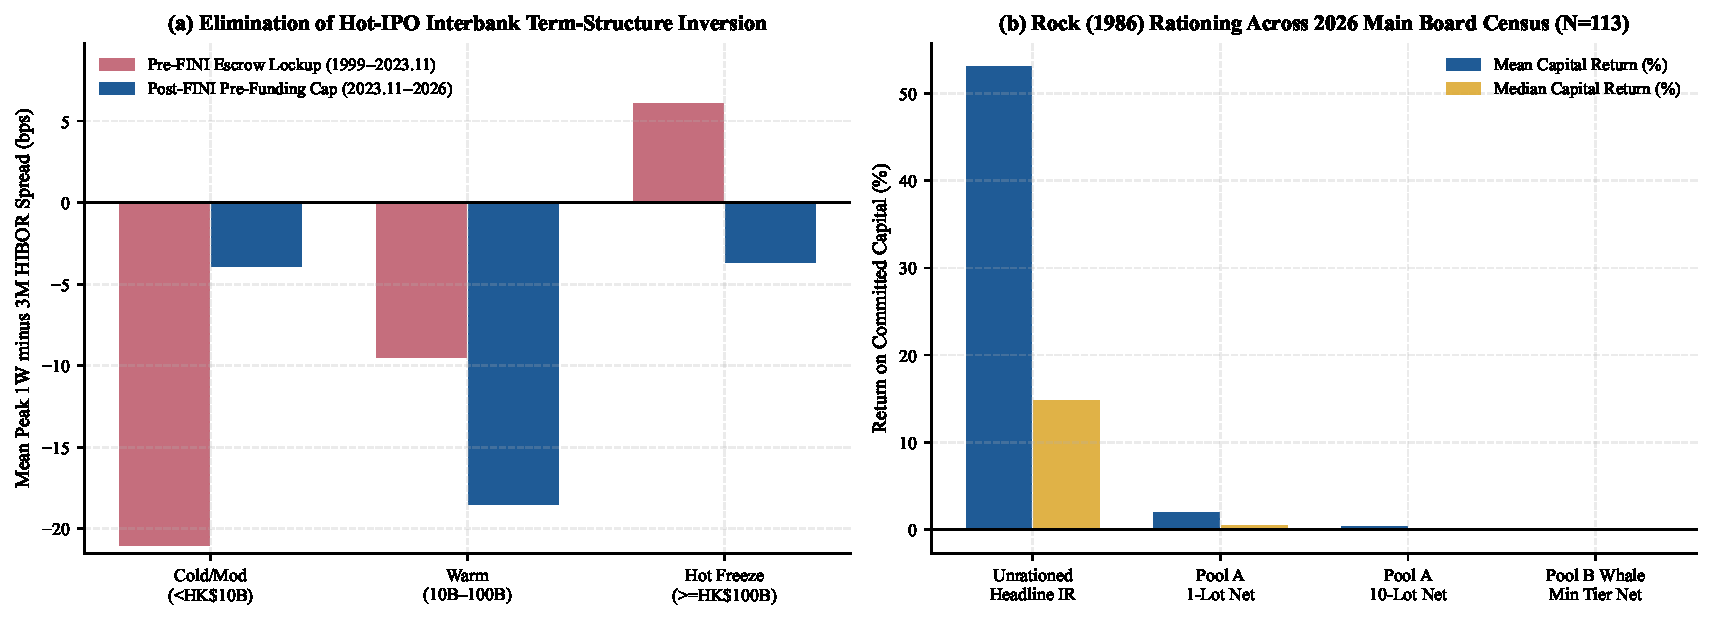
\includegraphics[width=\textwidth,height=0.80\textheight,keepaspectratio]{figures/journal_fig7.pdf}
\caption*{\textbf{Figure 7.2:} Fast Interface for New Issuance (FINI) settlement modernization and 2026 ballot-adjusted application returns. Panel (a) compares the mean peak 1-week minus 3-month Hong Kong Monetary Authority (HKMA) Hong Kong Interbank Offered Rate (HIBOR) spread across subscription capital tiers before versus after November 22, 2023 FINI implementation (1999–2026): during hot mega-subscriptions ($\ge$ HK\$100B), pre-FINI cash escrow lockups inverted the short-term money-market curve (+6.1 bp), whereas post-FINI credit-cap confirmations keep the mega-IPO spread negative (-3.7 bp, eliminating the \textasciitilde{}10 bp inversion, though indistinguishable from macro rate cycles within the narrow 2021–2026 window). Panel (b) contrasts first-day returns from the offer price (+53.15\% mean / +14.82\% median) against net returns per dollar applied for (after 1.0085\% statutory fees and 3-day 90\% FINI margin interest at 3.80\% p.a.) across Pool A one-lot (+1.97\% net mean), Pool A ten-lot (+0.35\%), and Pool B minimum-size financed application ($\ge$ HK\$5M, -0.06\%) strategies across all 113 Main Board IPOs in 2026Q1–Q3.}
\end{figure}

\subsection*{\texorpdfstring{7.4 Do Retail Investors Really Earn the First-Day Return?}{7.4 Do Retail Investors Really Earn the First-Day Return?}}
\addcontentsline{toc}{subsection}{\texorpdfstring{7.4 Do Retail Investors Really Earn the First-Day Return?}{7.4 Do Retail Investors Really Earn the First-Day Return?}}
A large first-day return from the offer price tells an applicant little about what they earned on the amount applied for. Seeing 2026 Main Board IPOs average a \textbf{+53.15\%} first-day return from the offer price, an observer might infer that public subscribers enjoy an easy primary-market arbitrage. Because an applicant earns returns only on shares \textit{allotted} rather than shares \textit{applied for}, the \textbf{gross return per dollar applied for} in any given order tier equals $(\text{fill rate}) \times (\text{first-day return from the offer price})$. Whenever fill rates are smaller in offerings with higher debut gains, the negative covariance between allocation and return compresses average application payoffs well below the first-day return from the offer price (Rock, 1986; Koh and Walter, 1989; Aggarwal, Prabhala, and Puri, 2002). Hong Kong's published allotment schedules allow us to compute those exact fill rates and \textbf{net returns per dollar applied for} across order sizes within the same offerings—holding offer price $P_0$ and Day-1 close $P_1$ fixed—by contrasting a small, ballot-favored cash application (Pool A, 1-lot) against a Pool B minimum-size financed application ($\ge$ HK\$5 million on 90\% FINI margin; Table 7.2).\footnote{Statutory primary subscription charges total 1.0085\% of allotted value (1.0\% brokerage, 0.0027\% SFC transaction levy, 0.00015\% AFRC transaction levy, and 0.00565\% HKEX trading fee). The detailed cost scenario in Table 7.2 also incorporates 0.1385\% secondary-sale stamp duty and levies, deal-specific 1-month HIBOR over the actual holding period (mean 4.4 days), and a HK\$100 broker margin handling fee.} Because a leveraged applicant posts only a fraction of the application amount in own cash, reporting returns strictly per dollar applied for (alongside explicit fee and financing assumptions) keeps the denominator uniform across cash and margin tiers.

\begin{table}[!htbp]
\centering
\caption*{Table 7.2 — 2026 Retail Ballot Census Across Investor Tiers with Explicit Denominators (N = 113 Main Board IPOs)}
\begin{adjustbox}{max width=\textwidth,max totalheight=0.79\textheight}
\begin{minipage}{\textwidth}\centering
\footnotesize
\setlength{\tabcolsep}{3.5pt}
\renewcommand{\arraystretch}{1.18}
\begin{adjustbox}{max width=\textwidth}
\begin{tabular}{>{\raggedright\arraybackslash}p{4.10cm}ccc>{\centering\arraybackslash}p{2.84cm}>{\centering\arraybackslash}p{1.90cm}>{\centering\arraybackslash}p{2.69cm}c}
\toprule
Investor Strategy / Pool Tier (2026Q1–Q3) & Deals ($N$) & Mean Fill Rate (\%) & Median Fill Rate (\%) & Gross Return per Dollar Applied For (\%) & Median Gross Return (\%) & Net Return per Dollar Applied For (\%) & Positive Net Deals (\%) \\
\midrule
\textbf{First-Day Return from Offer Price} \textit{(100\% Fill Benchmark)} & 113 & 100.00\% & 100.00\% & +53.15\% & +14.82\% & \textbf{+52.15\%} & 69.9\% \\
\textbf{Pool A: 1-Lot Cash Application} \textit{(Median Ticket HK\$4,358)} & 113 & 10.78\% & 3.00\% & +2.08\% & +0.59\% & \textbf{+1.97\%} & 69.9\% \\
\textbf{Pool A: 10-Lot Medium Retail Application} & 113 & 3.54\% & 0.86\% & +0.39\% & +0.18\% & \textbf{+0.35\%} & 69.9\% \\
\textbf{Pool B: Minimum-Size Financed Application} \textit{($\ge$ HK\$5M, 90\% FINI Margin)} & 111 & 2.01\% & \textbf{0.11\%} & -0.01\% & +0.02\% & \textbf{-0.06\%} & 40.5\% \\
\bottomrule
\end{tabular}
\end{adjustbox}
\end{minipage}
\end{adjustbox}
\par\vspace{3pt}\noindent\parbox{\textwidth}{\scriptsize\raggedright \textit{Notes}: Published Hong Kong Exchanges and Clearing (HKEX) Allotment Results schedules across all 113 Main Board IPOs completed in 2026Q1–Q3 (Pool B has $N = 111$ because two small offerings carried no Pool B tranche). \textit{Definitions}: $P_0$ is the IPO offer price, $P_1$ is the first-day closing price, and \textit{first-day return from the offer price} (Day-1 IR) is $(P_1 - P_0)/P_0$; \textit{Fill Rate} is shares allotted divided by shares applied for; \textit{Gross Return per Dollar Applied For} is $(\text{Fill Rate}) \times \text{Day-1 IR}$, using total application value (not allotted value or own cash posted) as the denominator. \textit{Net Return per Dollar Applied For} deducts statutory 1.0085\% primary subscription charges (brokerage, Securities and Futures Commission [SFC] and Accounting and Financial Reporting Council [AFRC] levies, and HKEX trading fee) on allotted value plus 3-day 90\% Fast Interface for New Issuance (FINI) margin interest at 3.80\% p.a. on financed Pool B applications. A detailed financing scenario using each deal's 1-month Hong Kong Interbank Offered Rate (HIBOR) and actual holding period (mean 4.4 days), a HK\$100 margin handling fee, and 0.1385\% sale costs leaves the 1-lot net return per dollar applied for in excess of HIBOR at +1.92\% (mean HK\$79, median HK\$19 per application) and the Pool B minimum-size financed application at -0.065\% when the full loan bears HIBOR (median -HK\$916 per application) or -0.035\% under a flat-fee margin package (median +HK\$756).}
\end{table}

If first-day returns from the offer price represented a scalable arbitrage, large financed applications would earn clearly positive net returns per dollar applied for. Evaluated per dollar applied for rather than per share allotted (Table 7.2), they earn approximately nothing. A Pool B minimum-size financed application ($\ge$ HK\$5 million) is rationed to a median \textbf{0.11\%} fill rate in heavily oversubscribed deals while receiving larger fills in weak ones, yielding a \textbf{-0.06\%} net return per dollar applied for after statutory fees and three days of margin interest at 3.80\%. The sign of that small number depends on how the loan is priced: with deal-specific HIBOR and holding periods the mean is -0.065\%, a median loss of about HK\$900 per application, whereas under a flat-fee margin package it is -0.035\% with a median \textit{gain} of about HK\$760. Either way, the net return per dollar applied for on a multi-million-dollar order is close to zero. A one-lot cash application retains a \textbf{+1.97\%} net return per dollar applied for, because ballot schedules tilt fill rates toward single-lot orders, but on a median ticket of HK\$4,358 that is an average of HK\$79 per application after funding costs and a median of HK\$19.

These magnitudes are consistent with Rock's (1986) rationing equilibrium. They do not by themselves establish its informational mechanism. In Hong Kong, fill rates fall with order size by rule and fall further in hot deals because demand is mechanically spread over a fixed tranche, whether or not large bidders are better informed. Distinguishing informed demand from mechanical rationing would require evidence on who bids, for example whether the same applicants systematically avoid weak deals.

\subsection*{\texorpdfstring{7.5 The Opening Auction, the Grey Market, and the First Month}{7.5 The Opening Auction, the Grey Market, and the First Month}}
\addcontentsline{toc}{subsection}{\texorpdfstring{7.5 The Opening Auction, the Grey Market, and the First Month}{7.5 The Opening Auction, the Grey Market, and the First Month}}
By the time the official opening auction runs, most of the first-day price movement has already occurred. Across 2,111 Main Board deals, the opening return and closing return are nearly identical, and regressing Day-1 close-to-offer returns on open-to-offer returns yields a slope of 0.99 ($R^2 = 0.78$; Table C.1), confirming that the official opening price is close to an unbiased forecast of the close (Biais, Hillion, and Spatt, 1999).

As institutional background, some pre-opening price discovery takes place the afternoon before listing (4:15 p.m. to 6:30 p.m., after allotment results are released) on broker-run over-the-counter \textbf{grey markets} (\textit{anpan}, led by Phillip Securities, Bright Smart, and Futu), where excess retail demand constrained by the top of the published offer range begins to clear ahead of the exchange bell. Because those platforms are fragmented across private brokers rather than consolidated on HKEX's historical tape, systematic 33-year grey-market quotes sit outside our census and remain a boundary for future high-frequency work.

After the debut, stabilization comes into play. For about 30 days under Cap. 571W, a stabilizing manager may support the shares at or below the offer price and use the over-allotment arrangement (Aggarwal, 2000). The return distribution shows a noticeable concentration at exactly the offer price (185 of 2,754 deals, or 6.7\%, closing within $\pm$0.05\% of $P_0$) and more deals just above it than just below. Part of that pattern reflects the mass at zero and price tick sizes, so we treat it as consistent with price support and do not attach a precise size to it. Some weak deals also lose ground once support ends, and non-A+H issues see daily trading value fall when the stabilization period expires.

Interpreting these mechanics requires separating long-run structure from recent cyclical conditions. The price ceiling, the clawback discontinuity, and the opening-auction result rest on long samples and are structural, whereas the ballot evidence is exact for 2026 only, when initial returns were cyclically elevated. Mechanism B and FINI likewise have short histories, and their observed effects remain entangled with a strong equity market. By the first-day close, an investor buying on the exchange faces a different price from an investor who received an allocation. We track both entry points to see how much they matter over the first year.

\par\medskip\noindent\rule{\linewidth}{0.35pt}\par\medskip
\section*{\texorpdfstring{Section 8. After the IPO: Who Actually Makes Money?}{Section 8. After the IPO: Who Actually Makes Money?}}
\addcontentsline{toc}{section}{\texorpdfstring{Section 8. After the IPO: Who Actually Makes Money?}{Section 8. After the IPO: Who Actually Makes Money?}}
\markright{Section 8. After the IPO}
Whether Hong Kong IPOs underperform depends critically on entry price, portfolio weighting, and historical period. Bought at the first-day close and held for one year, the average Main Board IPO trails the estimated dividend-reinvested Hang Seng benchmark by about 4 percentage points, while the median offering trails by roughly 20 percentage points. From the offer price, the average IPO exceeds the benchmark by nearly 5 percentage points, and weighting by proceeds eliminates most of the secondary-market shortfall. Over the full multi-decade horizon, roughly three-quarters of verified IPOs trade below their offer price, while a small minority of compounders generate most of the cumulative gain.

\subsection*{\texorpdfstring{8.1 One-Year Returns: The Answer Depends on the Entry Price}{8.1 One-Year Returns: The Answer Depends on the Entry Price}}
\addcontentsline{toc}{subsection}{\texorpdfstring{8.1 One-Year Returns: The Answer Depends on the Entry Price}{8.1 One-Year Returns: The Answer Depends on the Entry Price}}
Long-run IPO returns are notoriously sensitive to method (Ritter, 1991; Loughran and Ritter, 1995; Barber and Lyon, 1997; Fama, 1998; Mitchell and Stafford, 2000). Table 8.1 reports them against the Hang Seng price index, an estimated dividend-reinvested Hang Seng benchmark, and seasoned firms of similar size. The \textbf{estimated dividend-reinvested Hang Seng benchmark} compounds the Hang Seng price index with a fixed annual dividend yield for each calendar year, spread evenly across months. It is not the published Hang Seng total-return index, which does not cover the full period, and every dividend-reinvested benchmark comparison in this section inherits that approximation.

\begin{table}[p]
\centering
\caption*{Table 8.1 — One-Year Benchmark-Adjusted BHARs and Seasoned Calendar-Time Factor Alphas (1994–2026Q3)}
\begin{adjustbox}{max width=\textwidth,max totalheight=0.79\textheight}
\begin{minipage}{\textwidth}\centering
\par\noindent{\footnotesize\bfseries Panel A: 1-Year Buy-and-Hold Abnormal Returns — Hang Seng Price Index vs. Estimated Dividend-Reinvested Hang Seng Benchmark and Size-Matched Controls}\par\vspace{2pt}
\scriptsize
\setlength{\tabcolsep}{3.5pt}
\renewcommand{\arraystretch}{1.18}
\begin{adjustbox}{max width=\textwidth}
\begin{tabular}{>{\raggedright\arraybackslash}p{2.73cm}cc>{\centering\arraybackslash}p{2.78cm}>{\centering\arraybackslash}p{3.19cm}cccc}
\toprule
Board \& Epoch & Matured ($N$) & Raw 1Y Mean (\%) & BHAR vs. Hang Seng Price Index (\%) & BHAR vs. Est. Div.-Reinv. Hang Seng (\%) & $t_{\text{SA}}$ (Div.-Reinv.) & Size-Matched BHAR (\%) & $t_{\text{SA}}$ (Size) & Wealth Relative (Size) \\
\midrule
\textbf{Main Board — Era I (1994–1999)} & 190 & -2.57\% & -2.63\% & -6.07\% & -1.09 & -1.76\% & -0.31 & 0.982 \\
\textbf{Main Board — Era II (2000–2007)} & 341 & +14.46\% & +8.15\% & +4.81\% & +1.25 & -5.78\% & -1.37 & 0.952 \\
\textbf{Main Board — Era III (2008–2017)} & 660 & +6.49\% & +3.03\% & -0.59\% & -0.24 & -2.22\% & -0.92 & 0.980 \\
\textbf{Main Board — Era IV (2018–2022)} & 575 & -8.77\% & -2.89\% & -6.13\% & -2.03 & -6.96\% & -2.25 & 0.929 \\
\textbf{Main Board — Era V (2023–2026Q3)} & 210 & -7.38\% & -17.86\% & -22.25\% & -3.27 & -15.16\% & -2.45 & 0.859 \\
\textbf{All Main Board Matured 1Y} & \textbf{1,976} & \textbf{+1.08\%} & \textbf{-0.58\%} & \textbf{-4.10\%} & \textbf{-2.57} & \textbf{-5.55\%} & \textbf{-3.44} & \textbf{0.948} \\
\textbf{All GEM Matured 1Y} & \textbf{377} & \textbf{-12.33\%} & \textbf{-13.12\%} & \textbf{-16.56\%} & \textbf{-2.68} & \textbf{-19.50\%} & \textbf{-3.02} & \textbf{0.818} \\
\bottomrule
\end{tabular}
\end{adjustbox}
\par\vspace{5pt}
\par\noindent{\footnotesize\bfseries Panel B: Out-of-Sample Seasoned HKEX Three-Factor Calendar-Time Portfolio Alphas (1994–2026Q3)}\par\vspace{2pt}
\scriptsize
\setlength{\tabcolsep}{3.5pt}
\renewcommand{\arraystretch}{1.18}
\begin{adjustbox}{max width=\textwidth}
\begin{tabular}{>{\raggedright\arraybackslash}p{3.12cm}c>{\centering\arraybackslash}p{2.07cm}>{\centering\arraybackslash}p{2.40cm}>{\centering\arraybackslash}p{2.40cm}cccc}
\toprule
Calendar-Time Portfolio & Months ($T$) & CAPM-TR OLS $\alpha$ (\%/mo) & Seasoned 3F OLS $\alpha$ (\%/mo) & Seasoned 3F WLS $\alpha$ (\%/mo) & $\beta_{\text{MKT}}$ & $\beta_{\text{SMB}}$ & $\beta_{\text{MOM}}$ & $R^2$ \\
\midrule
\textbf{Main Board 12M Equal-Weighted} & 391 & +0.096\% (+0.30) & -0.432\% (-1.16) & \textbf{-0.651\%} (-2.11) & 0.89 & +0.67 & -0.13 & 0.542 \\
\textbf{Main Board 12M IPO-Proceeds-Weighted} & 391 & -0.215\% (-0.73) & -0.375\% (-1.08) & -0.447\% (-1.32) & 0.98 & +0.21 & -0.15 & 0.565 \\
\textbf{Main Board 36M Equal-Weighted} & 391 & -0.133\% (-0.45) & -0.598\% (-1.77) & \textbf{-0.625\%} (-2.37) & 0.85 & +0.59 & -0.20 & 0.584 \\
\textbf{Main Board 36M IPO-Proceeds-Weighted} & 391 & -0.043\% (-0.18) & -0.047\% (-0.17) & \textbf{-0.080\%} (-0.28) & 1.02 & +0.03 & -0.21 & 0.687 \\
\textbf{GEM 12M Equal-Weighted} & 200 & -1.039\% (-1.70) & -2.129\% (-3.24) & \textbf{-2.217\%} (-4.11) & 0.78 & +1.32 & +0.27 & 0.237 \\
\textbf{GEM 36M IPO-Proceeds-Weighted} & 275 & -0.555\% (-1.06) & -1.981\% (-3.47) & \textbf{-1.816\%} (-4.30) & 0.90 & +1.50 & +0.27 & 0.338 \\
\bottomrule
\end{tabular}
\end{adjustbox}
\par\vspace{5pt}
\par\noindent{\footnotesize\bfseries Panel C: Identical-Sample WLS Calendar-Time Alphas with Newey–West HAC(6) — 3F, 4F (+HML), 5F (+Illiquidity), and Forward-Cap HML Sensitivity (2001–2026Q3)}\par\vspace{2pt}
\footnotesize
\setlength{\tabcolsep}{3.5pt}
\renewcommand{\arraystretch}{1.18}
\begin{adjustbox}{max width=\textwidth}
\begin{tabular}{>{\raggedright\arraybackslash}p{2.66cm}c>{\centering\arraybackslash}p{1.90cm}>{\centering\arraybackslash}p{2.19cm}>{\centering\arraybackslash}p{2.69cm}>{\centering\arraybackslash}p{2.19cm}c>{\centering\arraybackslash}p{2.47cm}}
\toprule
Calendar-Time Portfolio & Months ($T$) & 3F WLS $\alpha$ ($t_{\text{HAC6}}$) & 4F (+HML) WLS $\alpha$ ($t_{\text{HAC6}}$) & Paired $\Delta\alpha_{4F-3F}$ ($t_{\text{HAC6}}$) & 5F (+LIQ) WLS $\alpha$ ($t_{\text{HAC6}}$) & $\beta_{\text{LIQ}}$ ($t_{\text{HAC6}}$) & Fwd-Cap HML $\Delta\alpha$ ($t_{\text{HAC6}}$) \\
\midrule
\textbf{Main Board 12M Equal-Weighted} & 303 & -0.653\% (-1.69) & -0.405\% (-1.10) & +0.247 pp (+2.51) & -0.407\% (-1.11) & -0.232 (-0.99) & -0.046 pp (-1.10) \\
\textbf{Main Board 12M IPO-Proceeds-Weighted} & 303 & -0.385\% (-0.82) & -0.058\% (-0.13) & +0.327 pp (+3.03) & -0.063\% (-0.14) & -0.496 (-2.18) & -0.005 pp (-0.15) \\
\textbf{Main Board 36M Equal-Weighted} & 303 & -0.396\% (-1.34) & -0.174\% (-0.65) & +0.222 pp (+2.50) & -0.175\% (-0.65) & -0.100 (-0.50) & -0.054 pp (-1.30) \\
\textbf{Main Board 36M IPO-Proceeds-Weighted} & 303 & -0.084\% (-0.23) & +0.210\% (+0.64) & +0.294 pp (+2.95) & +0.206\% (+0.62) & -0.343 (-1.97) & +0.011 pp (+0.33) \\
\textbf{GEM 12M Equal-Weighted} & 183 & \textbf{-1.942\%} (-3.45) & \textbf{-1.250\%} (-2.17) & +0.693 pp (+2.57) & \textbf{-1.270\%} (-2.29) & +0.332 (+1.84) & +0.009 pp (+0.15) \\
\textbf{GEM 36M Equal-Weighted} & 258 & \textbf{-1.471\%} (-3.10) & \textbf{-1.157\%} (-2.69) & +0.314 pp (+1.88) & \textbf{-1.142\%} (-2.79) & +0.415 (+2.22) & — \\
\bottomrule
\end{tabular}
\end{adjustbox}
\end{minipage}
\end{adjustbox}
\par\vspace{3pt}\noindent\parbox{\textwidth}{\scriptsize\raggedright \textit{Notes}: 33-year ordinary HKEX IPO census through November 12, 2026. Panel A computes 1-year buy-and-hold abnormal returns (BHAR) from Day-1 close ($P_1$) against the Hang Seng price index, the estimated dividend-reinvested Hang Seng benchmark, and size-matched seasoned HKEX firms listed $>3$ years, with Lyon, Barber, and Tsai (1999) skewness-adjusted $t_{\text{SA}}$ (listing-month-clustered all-Main-Board $t = -2.05$ vs. dividend-reinvested benchmark, $-2.86$ vs. size-matched). Panels B–C report monthly calendar-time alphas in \% per month and Panel C reports differences in pp per month. Parentheses contain $t$-statistics. \textbf{IPO-Proceeds-Weighted} weights active cohort IPOs each month by gross IPO proceeds, whereas cross-month \textbf{WLS} regression weighting weights month $t$ by $\sqrt{N_t}$ ($N_t$ = active IPOs in month $t$). Panel B uses CAPM total-return excess returns (CAPM-TR) and seasoned HKEX market (MKT), size (SMB), and momentum (MOM) factors with OLS and WLS (HC3 SEs). Panel C adds seasoned book-to-market value (HML) and an illiquidity factor based on trailing-12-month months with zero returns (LIQ; Lam and Tam, 2011) on identical overlapping months (2001–2026Q3) using $\sqrt{N_t}$ WLS with 6-lag Newey–West HAC(6) SEs and stacked GMM paired $\Delta\alpha$ tests; the last column replaces HML using market values inferred from current capitalization with strictly forward-cast listing-cap HML (zero share-count look-ahead).}
\end{table}

Table 8.1 immediately confronts two opposing readings of Hong Kong's aftermarket record. Seeing mean one-year BHARs for matured Main Board IPOs ($N = 1,976$) of \textbf{-4.10\%} against the estimated dividend-reinvested Hang Seng benchmark ($t_{\text{SA}} = -2.57$) and \textbf{-5.55\%} against size-matched seasoned peers ($t_{\text{SA}} = -3.44$), a behavioral critic might conclude that Hong Kong's entire primary market systematically destroys investor wealth. Conversely, another reading attributes negative equal-weighted IPO returns to omitted benchmark dividends, portfolio weighting choices, and size, value, or illiquidity risk factors. Disentangling those two stories requires testing four distinct economic mechanisms sequentially.

First, we shift the entry point from the first-day close ($P_1$) back to the offer price ($P_0$). The sign reverses: from the $P_0$ entry price, the one-year BHAR against the estimated dividend-reinvested Hang Seng benchmark was \textbf{+4.9\%} equal-weighted and \textbf{+9.3\%} proceeds-weighted (actual allocations are unobserved, and rationing changes what applicants realize; Section 7.4). The reversal is largely an identity. For the same stock and end date, $1 + R_{P_0} = (1 + \text{IR})(1 + R_{P_1})$, so a positive average first-day return mechanically lifts the offer-price return above the first-day-close return. The comparison shows how much the entry price is worth to an investor; it does not show, on its own, that secondary buyers paid more than the shares were fundamentally worth, since the same pattern arises if the offer price was set low and the debut price was fair.

Second, to test whether aftermarket underperformance is a \textbf{structural market failure} or a product of \textbf{cyclical hot-issue sentiment and market timing}, we compare historical issuance regimes across eras. If structural mispricing prevailed uniformly, mean underperformance would appear in every period. Instead, cohorts listed across 1994–2017 roughly matched the total-return benchmark on an equal-weighted mean basis, whereas negative pooled means arise almost entirely from Era IV (-6.13\%, $t_{\text{SA}} = -2.03$) and Era V (-22.25\%, $t_{\text{SA}} = -3.27$), when hot debuts reversed against strong index rallies. Median underperformance, by contrast, is pervasive across every era, foreshadowing the extreme right-tail skewness examined in Section 8.2.

Third, to test the strongest efficient-market counterargument—that negative equal-weighted returns merely reflect \textbf{small-cap, value, and illiquidity risk factors} rather than genuine value destruction—we compare IPO-proceeds-weighted against equal-weighted calendar-time portfolios and juxtapose the tightly screened Main Board against the lightly screened junior board (GEM) across seasoned three-, four-, and five-factor models (Table 8.1, Panels B–C; Fama and French, 1993; Lyon, Barber, and Tsai, 1999). If omitted risk premiums explained IPO returns, adding local size, book-to-market, momentum, and zero-return illiquidity factors should extinguish abnormal alphas on \textit{both} boards. The results split cleanly by proceeds weighting and screening discipline. On the Main Board, weighting by IPO proceeds eliminates abnormal underperformance completely: proceeds-weighted multi-year alphas are statistically indistinguishable from zero under every factor specification. Modest negative three-factor intercepts appear only in equal-weighted Main Board portfolios driven by smaller listings, and while adding a local book-to-market factor shifts those intercepts toward zero, robustness checks show that marginal shift depends on how historical capitalization is reconstructed (Table 8.1 Notes and Appendix C.3). GEM, by contrast, continues to exhibit statistically significant negative alphas under every factor model estimated here: even after adjusting for market, size, momentum, value, and illiquidity, five-factor alphas remain deeply negative—roughly \textbf{-14.2\% annualized} over one year (-1.27\% per month) and \textbf{-12.9\% annualized} over three years (-1.14\% per month; Table 8.1, Panel C)—pointing to persistent risk-adjusted underperformance on the lightly screened junior board.

Fourth, even on the Main Board, cross-sectional return dispersion after listing could simply reflect unforeseen post-IPO business shocks rather than \textbf{asymmetric information and opportunistic pre-IPO earnings management} that primary-market investors fail to unpack (Teoh, Welch, and Wong, 1998). Because realized operating cash flows are far harder to inflate than accounting accruals, pre-IPO total accruals scaled by assets proxy for the extent to which reported prospectus earnings depend on reversible accounting judgments rather than cash generation. If investors rationally priced earnings quality at the offering, issuers relying heavily on non-cash accruals would be discounted on Day 1 and exhibit no systematic post-listing reversal. In the closely reviewed 2025–2026 cohort ($N = 225$, partitioned into three equal 75-firm accrual tiers), the data tell the opposite story. Issuers in the lowest-accrual tier (median accruals -13.11\% of assets; median operating cash flow to net profit of 2.28x) and the highest-accrual tier (median accruals +3.10\% of assets; cash conversion 0.45x, a gap partly mechanical by construction) record virtually identical mean first-day returns (+45.92\% versus +45.23\%)—showing that debut pricing largely overlooks accrual quality. Only over the ensuing six months, as underlying cash flows materialize, does the mispricing unwind: low-accrual issuers earn a mean raw buy-and-hold return of \textbf{+25.80\%} ($N = 53$) compared with \textbf{+0.19\%} ($N = 51$) for high-accrual issuers, a 25.61 percentage-point divergence. Appendix C.2 tests two sharper proxies for discretionary accounting choices—IAS 38 R\&D capitalization and thin-margin issuers sitting near the Main Board profit gate—and finds parallel directional gaps; as noted there, all six-month figures reflect raw returns over a short, cyclically elevated window.

The one-year results change when larger deals receive more weight. That raises a longer-run question: how much of the market’s aggregate gain came from its biggest winners?

\subsection*{\texorpdfstring{8.2 The Big Reconciliation: Most IPOs Lose, the Total Is Large}{8.2 The Big Reconciliation: Most IPOs Lose, the Total Is Large}}
\addcontentsline{toc}{subsection}{\texorpdfstring{8.2 The Big Reconciliation: Most IPOs Lose, the Total Is Large}{8.2 The Big Reconciliation: Most IPOs Lose, the Total Is Large}}
Two distinct mechanisms reconcile Hong Kong's seemingly contradictory return statistics. Whereas \textbf{entry price} ($P_0$ versus $P_1$) explains why investors buying at the offer price and buyers entering at the first-day close earn opposite one-year average excess returns, \textbf{extreme right-tail skewness} (the same mechanism Bessembinder, 2018 documents for U.S. equities) explains how most individual offerings lose money while the shares sold at IPO still generate HK\$3.71 trillion in cumulative net price appreciation before dividends. Across 2,117 split-verified terminal offerings (Table 8.2; money totals use the 2,116 with recorded proceeds), the median IPO sits \textbf{63.20\%} below its offer price and \textbf{77.47\%} (roughly three-quarters) trade below $P_0$, yet the top 1\% of issuers (just 21 companies) generated \textbf{73.77\%} of all gross positive gains among appreciating offerings, with Tencent alone contributing \textbf{+HK\$1,093.2 billion} (29.5\% of the net market total). Meanwhile, GEM generated a net cumulative loss of \textbf{-HK\$13.2 billion}, with 90.85\% of verified listings trading below offer. Throughout, these aggregates measure performance at the level of shares sold at IPO; estimating realized returns for specific investors requires separate evidence on actual allocations and holding periods.

\begin{figure}[htbp]
\centering
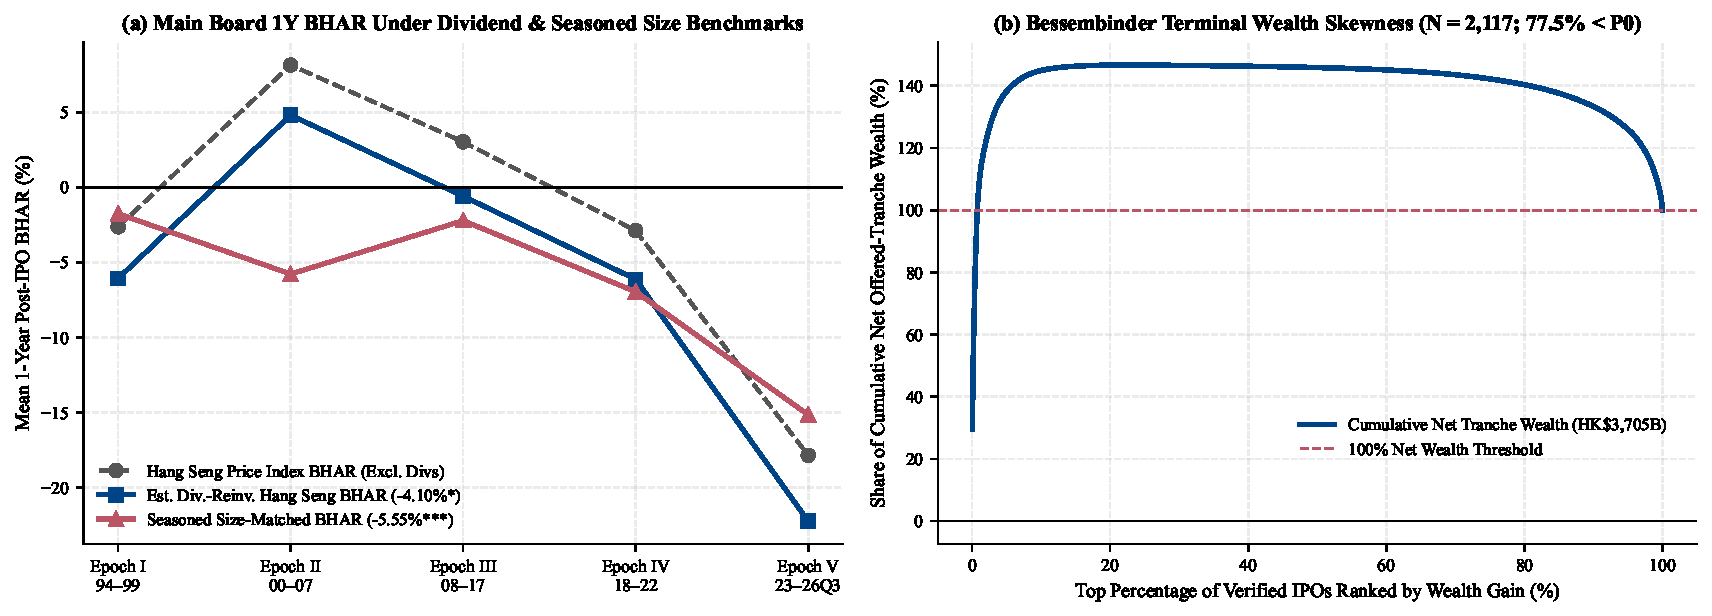
\includegraphics[width=\textwidth,height=0.80\textheight,keepaspectratio]{figures/journal_fig8.pdf}
\caption*{\textbf{Figure 8.1:} Long-run abnormal performance and lifetime offered-tranche wealth concentration, 1994–2026Q3 (through November 12, 2026). Panel (a) compares Main Board 1-year equal-weighted buy-and-hold abnormal returns (BHAR) from Day-1 close ($P_1$; $N = 1,976$ matured offerings) across five eras against the Hang Seng price index, the estimated dividend-reinvested Hang Seng benchmark, and seasoned size-matched controls, showing that Main Board cohorts roughly tracked the estimated dividend-reinvested Hang Seng benchmark across Eras I–III before Era IV (-6.13\%) and Era V (-22.25\%) drove the pooled mean to -4.10\% (estimated dividend-reinvested benchmark) and -5.55\% (size-matched). Panel (b) plots the empirical cumulative offered-tranche price-gain curve before dividends across all $N = 2,117$ split-verified terminal IPOs (from offer price $P_0$), showing that even though 77.5\% finish below $P_0$, the top 1\% (21 issuers) generate 73.8\% of gross gains among appreciating offerings.}
\end{figure}

\begin{table}[!htbp]
\centering
\caption*{Table 8.2 — Lifetime Return Skewness and Offered-Tranche Price Appreciation Concentration (to Nov 12, 2026)}
\begin{adjustbox}{max width=\textwidth,max totalheight=0.79\textheight}
\begin{minipage}{\textwidth}\centering
\scriptsize
\setlength{\tabcolsep}{3.5pt}
\renewcommand{\arraystretch}{1.18}
\begin{adjustbox}{max width=\textwidth}
\begin{tabular}{>{\raggedright\arraybackslash}p{3.80cm}cccccc>{\centering\arraybackslash}p{2.18cm}>{\centering\arraybackslash}p{2.72cm}}
\toprule
Terminal Wealth Universe & Verified (N) & Mean Raw Return (\%) & Median Raw Return (\%) & Below Offer ($<P_0$, \%) & Lost $\ge 80\%$ (\%) & 10-Baggers (\%) & Net Tranche Gain (HK\$B) & Top 1\% Share of Gross Gain (\%) \\
\midrule
\textbf{All HKEX Verified IPOs (1994–2026)} & \textbf{2,117} & +50.36\% & \textbf{-63.20\%} & \textbf{77.47\%} & 34.44\% & 1.75\% & \textbf{+3,705.5} & \textbf{73.77\%} \\
\textbf{HKEX Main Board} & 1,833 & +66.97\% & -58.15\% & 75.40\% & 30.93\% & 1.96\% & +3,718.6 & 71.07\% \\
\textbf{HKEX GEM} & 284 & -56.83\% & -84.41\% & \textbf{90.85\%} & \textbf{57.04\%} & 0.35\% & \textbf{-13.2} & 50.65\% \\
\textbf{Seasoned Cohorts $\ge 5$ Years (1994–2021)} & 1,693 & +63.79\% & -69.64\% & 77.85\% & 39.81\% & 2.01\% & +3,819.4 & 72.04\% \\
\bottomrule
\end{tabular}
\end{adjustbox}
\end{minipage}
\end{adjustbox}
\par\vspace{3pt}\noindent\parbox{\textwidth}{\scriptsize\raggedright \textit{Notes}: Across all 2,117 split-verified Hong Kong Exchanges and Clearing (HKEX) IPOs through November 12, 2026, the median offering sits \textbf{63.20\% below its offer price ($P_0$)} and \textbf{77.47\% trade below $P_0$} (rising to 90.85\% on the Growth Enterprise Market [GEM], which records a -HK\$13.2B net loss), yet extreme right-tail skewness generates +HK\$3,705.5B in cumulative net offered-tranche price appreciation before dividends because the top 1\% (21 issuers) account for 73.77\% of gross gains among appreciating offerings. \textit{Source}: Split-adjusted terminal pricing through November 12, 2026 (Appendix A audits attrition from 2,866 to 2,117). Returns are price changes before dividends. Sensitivity checks for 475 delisted issuers lacking terminal quotes keep the median return between -59.21\% and -75.71\% and the below-offer share between 75.69\% and 81.60\%.}
\end{table}

Benchmarking that HK\$3.71 trillion total against passive deployment into the Hang Seng Index on each listing date clarifies both the scale and the measurement boundaries of IPO wealth creation (Table 8.3). Defining the \textbf{wealth ratio} as terminal IPO-tranche value divided by terminal benchmark value, the index would have gained HK\$592.4 billion on a matching price-only basis, yielding a wealth ratio against the Hang Seng price index of \textbf{1.57} (1.37 excluding Tencent; 1.29 excluding both Tencent and AIA). Against the estimated dividend-reinvested Hang Seng benchmark (HK\$4,237.3 billion), price-only IPO gains trail at an asymmetric descriptive ratio of \textbf{0.94} (\textbf{0.82} excluding Tencent), and only \textbf{20.8\%} of offerings beat the Hang Seng price index individually. Using stock returns with dividends reinvested from Day 1 across \textbf{2,115 matched verified issuers} restores dividend symmetry: cumulative IPO gains climb to \textbf{+HK\$7,035.4 billion} against HK\$4,236.4 billion in the estimated dividend-reinvested Hang Seng benchmark, lifting the \textbf{like-for-like wealth ratio (stock returns with dividends reinvested versus the estimated dividend-reinvested Hang Seng benchmark) to 1.306} (\textbf{1.187} excluding Tencent; \textbf{1.139} excluding both Tencent and AIA), as cash-dividend compounders such as major PRC banks, China Mobile, and CNOOC add over HK\$3.3 trillion in reinvested distributions.

\begin{table}[!htbp]
\centering
\caption*{Table 8.3 — Offered-Tranche Gains Against the Same Dollars in the Hang Seng Index (to Nov 12, 2026)}
\begin{adjustbox}{max width=\textwidth,max totalheight=0.79\textheight}
\begin{minipage}{\textwidth}\centering
\scriptsize
\setlength{\tabcolsep}{3.5pt}
\renewcommand{\arraystretch}{1.18}
\begin{adjustbox}{max width=\textwidth}
\begin{tabular}{lccc>{\centering\arraybackslash}p{2.00cm}>{\centering\arraybackslash}p{2.24cm}>{\centering\arraybackslash}p{2.30cm}>{\centering\arraybackslash}p{2.53cm}>{\centering\arraybackslash}p{2.24cm}}
\toprule
Cohort & Verified IPOs ($N$) & Proceeds (HK\$B) & IPO Price Gain (HK\$B) & Hang Seng Price Index Gain (HK\$B) & Wealth Ratio vs. Hang Seng Price Index & Est. Div.-Reinv. Hang Seng Gain (HK\$B) & Wealth Ratio vs. Est. Div.-Reinv. Hang Seng & IPOs Beating Hang Seng Price Index (\%) \\
\midrule
\textbf{Era I (1994–1999)} & 123 & 115.5 & +383.6 & +123.0 & 2.09 & +548.1 & 0.75 & 26.0\% \\
\textbf{Era II (2000–2007)} & 312 & 946.0 & +3,501.4 & +471.3 & 3.14 & +2,100.9 & 1.46 & 25.6\% \\
\textbf{Era III (2008–2017)} & 691 & 1,734.5 & +315.8 & +110.6 & 1.11 & +1,325.0 & 0.67 & 16.9\% \\
\textbf{Era IV (2018–2022)} & 640 & 1,382.6 & -432.3 & -110.9 & 0.75 & +233.2 & 0.59 & 20.3\% \\
\textbf{Era V (2023–2026Q3)} & 350 & 736.1 & -62.9 & -1.6 & 0.92 & +30.1 & 0.88 & 23.1\% \\
\textbf{All Verified IPOs} & \textbf{2,116} & \textbf{4,914.5} & \textbf{+3,705.5} & \textbf{+592.4} & \textbf{1.57} & \textbf{+4,237.3} & \textbf{0.94} & \textbf{20.8\%} \\
\textbf{All Excluding Tencent} & 2,115 & 4,912.8 & +2,612.2 & +590.7 & 1.37 & +4,231.3 & 0.82 & 20.8\% \\
\bottomrule
\end{tabular}
\end{adjustbox}
\par\vspace{5pt}
\par\noindent{\footnotesize\bfseries Panel B: Stock Returns with Dividends Reinvested and 475 Unquoted Delisting Bounds}\par\vspace{2pt}
\footnotesize
\setlength{\tabcolsep}{3.5pt}
\renewcommand{\arraystretch}{1.18}
\begin{adjustbox}{max width=\textwidth}
\begin{tabular}{>{\raggedright\arraybackslash}p{3.56cm}cc>{\centering\arraybackslash}p{2.36cm}>{\centering\arraybackslash}p{2.56cm}>{\centering\arraybackslash}p{2.82cm}cc}
\toprule
Dividend-Reinvested Scenario & Issuers ($N$) & Proceeds (HK\$B) & IPO Gain w/ Dividends Reinv. (HK\$B) & Est. Div.-Reinv. Hang Seng Gain (HK\$B) & Wealth Ratio vs. Est. Div.-Reinv. Benchmark & Excl. Tencent & Excl. Tencent \& AIA \\
\midrule
\textbf{Verified Matched (Stock Returns w/ Dividends Reinv.)} & \textbf{2,115} & \textbf{4,914.4} & \textbf{+7,035.4} & \textbf{+4,236.4} & \textbf{1.306} & \textbf{1.187} & \textbf{1.139} \\
\textbf{+ 475 Unquoted Delistings (363 Obs. + 0\% Rem.)} & 2,590 & 5,246.2 & +6,910.6 & +4,665.6 & \textbf{1.227} & 1.117 & 1.070 \\
\textbf{+ 475 Unquoted Delistings (363 Obs. + 100\% Rem.)} & 2,590 & 5,246.2 & +6,939.5 & +4,665.6 & \textbf{1.229} & 1.119 & 1.073 \\
\textbf{+ 475 Unquoted Delistings (All at 50\% Recovery)} & 2,590 & 5,246.2 & +6,869.5 & +4,665.6 & \textbf{1.222} & 1.112 & 1.066 \\
\textbf{+ 475 Unquoted Delistings (All Total Loss)} & 2,590 & 5,246.2 & +6,703.6 & +4,665.6 & \textbf{1.206} & 1.096 & 1.048 \\
\bottomrule
\end{tabular}
\end{adjustbox}
\end{minipage}
\end{adjustbox}
\par\vspace{3pt}\noindent\parbox{\textwidth}{\scriptsize\raggedright \textit{Notes}: \textit{Main benchmark result}: On a matching price-only basis (Panel A), verified IPO offered tranches outperform passive deployment in the Hang Seng price index at a \textbf{1.57$\times$ wealth ratio} (+HK\$3,705.5B vs. +HK\$592.4B, led by Era II at 3.14$\times$), though only 20.8\% of offerings beat the Hang Seng price index individually and omitting IPO dividends pulls the asymmetric comparison against the estimated dividend-reinvested Hang Seng benchmark to 0.94$\times$; restoring dividend symmetry via stock returns with dividends reinvested (Panel B, $N = 2,115$) lifts the like-for-like wealth ratio to \textbf{1.306$\times$} (1.187$\times$ excluding Tencent), remaining above parity at \textbf{1.227$\times$–1.229$\times$} (1.117$\times$–1.119$\times$ excluding Tencent) when the last pre-delisting quote stands in for the exit value of 363 unquoted delistings and the other 112 are bounded at 0\%–100\%, and at \textbf{1.206$\times$} (1.048$\times$ excluding Tencent and AIA) if all 475 are treated as total losses. \textit{Source \& definitions}: 33-year ordinary IPO census paired with the Hang Seng price index and estimated dividend-reinvested Hang Seng benchmark through November 12, 2026. All stock price and return series are adjusted for share splits and consolidations. Each IPO's proceeds are invested in the benchmark at the listing-date close; the \textit{wealth ratio} is terminal IPO-tranche value divided by terminal benchmark value. Panel A reports split-adjusted price changes excluding dividends (one verified terminal record lacks usable proceeds). Panel B chains split- and cash-dividend-reinvested stock return series from Day 1 across 2,115 matched verified issuers plus 363 unquoted delistings with observed pre-delisting quotes (median -86.0\%) and 0\%–100\% recovery bounds on the residual 112 unquoted offerings; the two final Panel B rows instead assign all 475 a flat 50\% or 0\% recovery of offer value. The estimated dividend-reinvested Hang Seng benchmark compounds the Hang Seng price index with annual dividend yields, and a further 274 offerings (HK\$413.1B) with recycled tickers, unadjusted consolidations, or unverified split factors are outside every row.}
\end{table}

Two immediate identification concerns confront Table 8.3's aggregate wealth numbers. First, seeing \textbf{Era II (2000–2007)} (+HK\$3,501.4 billion; 3.14x vs. the Hang Seng price index, 1.46x vs. the estimated dividend-reinvested Hang Seng benchmark) tower over \textbf{Eras IV–V (2018–2026)} (-HK\$495.2 billion combined), one could dismiss the cohort gap as a mechanical artifact of \textbf{compounding duration}—or a single-stock \textit{Tencent} anomaly—since Era II listings simply enjoyed two decades of compounding while modern cohorts are young. Placing every cohort on \textbf{identical standardized holding horizons} cleanly rules out both objections: Era II's proceeds-weighted outperformance over the estimated dividend-reinvested Hang Seng benchmark already opens within 3 years (1.32x, or 1.32x excluding Tencent) and widens at 5 years (\textbf{1.31x}, or \textbf{1.29x} excluding Tencent, compared with 0.91x in Era III and 0.62x in Era IV; full 1Y/3Y/5Y horizon grid in Appendix C.3). What completed listings still cannot separate—absent private-round valuation histories or buyout payoffs—is how much of the post-2018 shortfall reflects late-stage private investors capturing growth pre-IPO versus post-2018 macro cycles and issuer-mix shifts.

Second, aggregate wealth ratios could reflect \textbf{survivorship}, because the verified terminal panel omits 749 of the 2,866 IPOs. They fall into two groups with different treatments. \textbf{475 delisted issuers lack terminal quotes} (HK\$331.8 billion in proceeds). For 363 of them we observe a last quote before delisting (a median loss of 86\%) but not the cash paid at exit; 112 have no usable series at all. A further \textbf{274 offerings} (HK\$413.1 billion) are excluded because of recycled ticker codes or transfers (211; HK\$304.5 billion), unadjusted share consolidations (54; HK\$105.8 billion), or unverified split factors (9; HK\$2.8 billion), and no recovery scenario covers them. Table 8.3, Panel B reports the delisting scenarios side by side. Treating the last quote as the exit value for the 363 and bounding the other 112 between 0\% and 100\% gives a dividend-adjusted wealth ratio of 1.227–1.229, but that range varies only the 112. Assigning all 475 a flat 50\% recovery gives 1.222, and treating all 475 as total losses gives \textbf{1.206}, or 1.096 without Tencent and 1.048 without both Tencent and AIA. The excess over the benchmark therefore survives the harshest delisting assumption for the sample we can measure, but it is small once the two largest winners are removed, it relies on an estimated benchmark, and it says nothing about the 274 excluded offerings, whose outcomes could move it in either direction. Table 8.3 also mixes multi-decade holding periods with cohorts only months old and records appreciation on offered shares rather than realized returns for any investor group; buyout premiums paid at delisting remain unobserved. The fact that holds across every scenario is concentration: most offerings lose, and a handful account for most of the gain.

Whether investors can actually enter, hold, or exit those shares after listing depends on secondary-market tradability. The next three subsections follow that liquidity lifecycle in order: when locked-up shares reach the market (Section 8.3), whether daily trading endures past the debut (Section 8.4), and whether Stock Connect broadens the buyer base and narrows cross-border price gaps (Section 8.5).

\subsection*{\texorpdfstring{8.3 Lockups: Why Legal Form Changes the Supply Calendar}{8.3 Lockups: Why Legal Form Changes the Supply Calendar}}
\addcontentsline{toc}{subsection}{\texorpdfstring{8.3 Lockups: Why Legal Form Changes the Supply Calendar}{8.3 Lockups: Why Legal Form Changes the Supply Calendar}}
Lockup expiry adds shares at a known date, yet prices often weaken around it (Field and Hanka, 2001; Brav and Gompers, 2003). Hong Kong gives an unusual comparison. In many offshore-incorporated issuers, cornerstone and pre-IPO investor shares can come free around six months. In PRC-incorporated issuers, Company Law freezes pre-IPO shares for a year, so only the cornerstone shares are released at six months.

\begin{figure}[htbp]
\centering
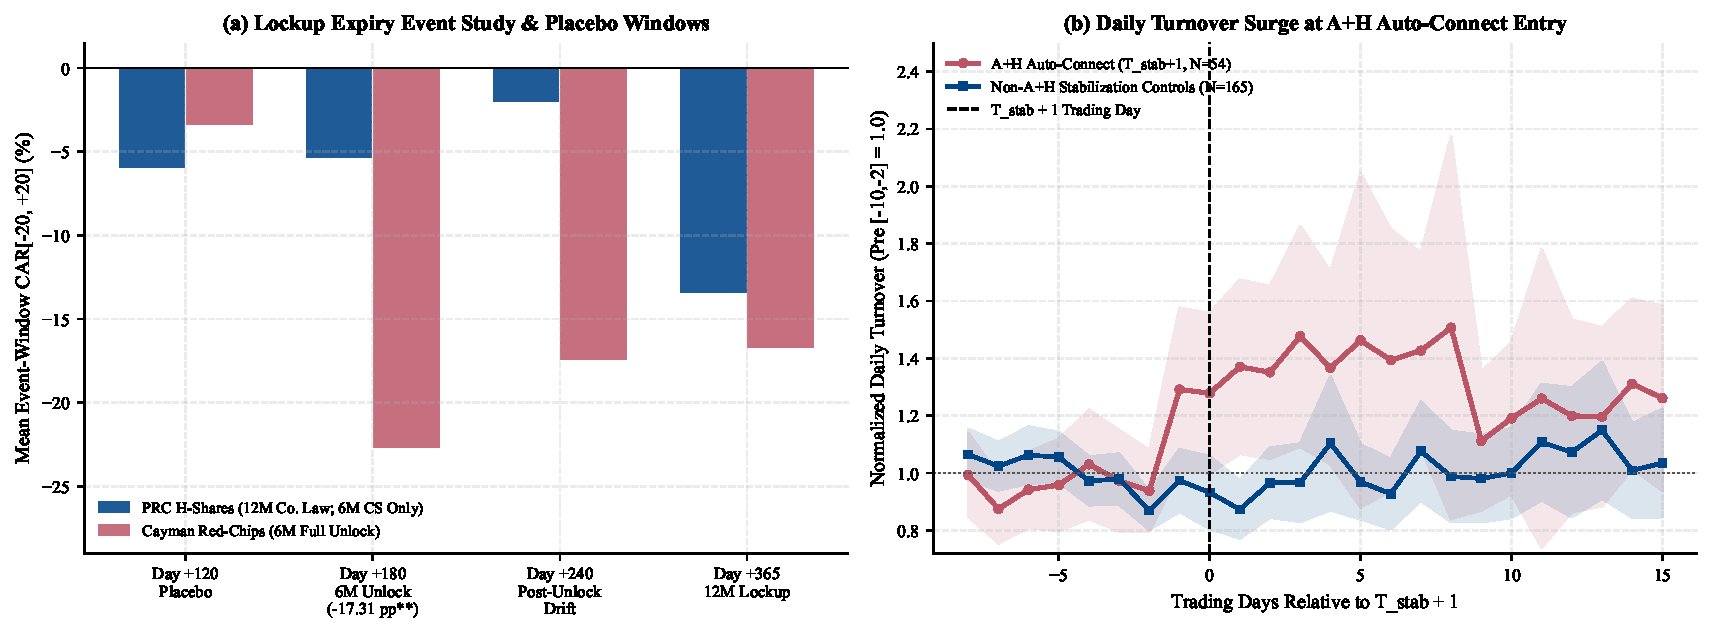
\includegraphics[width=\textwidth,height=0.80\textheight,keepaspectratio]{figures/journal_fig9.pdf}
\caption*{\textbf{Figure 8.2:} Jurisdictional lockup event studies with placebo windows and A+H automatic Stock Connect daily trading value paths (2025Q1–2026Q3). Panel (a) compares mean Hang Seng Index (HSI)-adjusted cumulative abnormal returns, $\text{CAR}(-20, +20)$ summed over trading days -20 to +20 around each calendar milestone (where Day 0 is the IPO listing date and Day +120, +180, +240, and +365 count \textbf{calendar days} post-listing, corresponding to 4, 6, 8, and 12 months), for People's Republic of China (PRC) H-shares versus Cayman offshore red-chips: because the post-unlock placebo gap at Day +240 (-15.43 pp, $p = 0.028$) is nearly as large as the six-month Day +180 gap (-17.31 pp, $t = -2.39$) and paired Day +365 differentials fail to reverse, \textbf{the divergence reflects persistent post-listing issuer-mix drift rather than an expiry-specific lockup sell-off}. Panel (b) plots daily trading value normalized to each issuer's pre-event trading days -10 through -2 mean (= 1.0) with 95\% confidence bands in trading days relative to $T_{\text{stab}} + 1$ (the first trading day after 30-day Cap. 571W price stabilization ends): automatic A+H Southbound Connect entrants ($N = 54$) experience a \textbf{+0.307 log-point (\textasciitilde{}36\%) relative jump in daily trading value} ($t = 3.32$; +0.294 with Greenshoe controls) versus non-A+H Main Board controls ($N = 165$), alongside a modest pre-admission upward drift (+0.044 log points/day).}
\end{figure}

At first glance, the headline jurisdictional split looks like textbook evidence of \textbf{downward-sloping demand curves and unlock-day supply pressure}: Cayman issuers in our recent sample fall 17.3 percentage points more steeply around Month 6 (-22.7\%, $N=32$) than PRC H-share issuers (-5.4\%, $N=91$; Figure 8.2a), show no pre-unlock gap at Day 120, and non-A+H H-share firms then weaken around Month 12 (-19.1\%) when their statutory Company Law lockups expire. Yet that headline contrast does not settle whether the Day-180 drop isolates \textbf{unlock-day selling pressure} or merely reflects \textbf{persistent issuer-selection drift}, with offshore Cayman issuers underperforming PRC H-shares continuously after listing. If temporary supply pressure were the true mechanism, the Cayman drag would vanish once Month-6 shares cleared, reverse cleanly when PRC lockups expire at Month 12, and scale in proportion to the \textbf{fraction of locked shares actually released}. All three falsification tests reject the supply-shock story: the Cayman drag persists virtually unchanged two months after expiry (\textbf{-15.4 percentage points} at Day 240), fails to reverse across Month 6 to Month 12 among paired issuers reaching both horizons, and neither abnormal returns nor daily trading value at Day 180 moves significantly with the actual fraction of locked shares released (full placebo, paired-DiD, and exposure-regression estimates are reported in Table C.1 and Appendix C.3). Those diagnostics cleanly overturn a naive supply-pressure reading: the Day-180 Cayman–PRC gap reflects persistent issuer-mix differences and post-listing drift rather than exposure-scaled selling at expiry.

The lockup calendar tells us when more shares can become available for trading. We now ask which stocks retain active trading after the debut.

\subsection*{\texorpdfstring{8.4 Where Does the Liquidity Go?}{8.4 Where Does the Liquidity Go?}}
\addcontentsline{toc}{subsection}{\texorpdfstring{8.4 Where Does the Liquidity Go?}{8.4 Where Does the Liquidity Go?}}
First-day trading is intense and rarely lasts: in most eras, a large majority of Main Board IPOs lose more than 95\% of their first-day trading volume by Month 6, many record days with zero trades, and GEM fares worse still (Figure 8.3a). Because debut trading volume is artificially elevated everywhere as initial allocations change hands, a steep post-listing trading volume drop could merely represent harmless mean reversion rather than a structural liquidity friction. If post-listing illiquidity instead reflects \textbf{market-making fixed costs, tradable-float scarcity, and investor participation barriers}, then the long tail of chronically untraded stocks should track structural constraints on supply and order flow rather than falling uniformly across issuers. Three microstructure proxies confirm that channel: larger offerings, which support dedicated institutional coverage and spread fixed market-making costs, preserve liquidity better on the Amihud (2002) price-impact measure; syndicates incorporating online retail brokers lower individual participation frictions and experience fewer zero-volume trading days; and offerings carrying heavy six-month cornerstone lockups directly restrict unrestricted secondary float and suffer thinner trading afterward. The informative signal is therefore not the decline from Day-1 trading volume itself, but how primary distribution choices and scale barriers leave a long tail of issues barely traded.

Trading thins for many firms after listing. Stock Connect lets us ask whether access to a broader buyer base is accompanied by higher daily trading value and a narrower price gap.

\subsection*{\texorpdfstring{8.5 Stock Connect: More Trading, Not One Market}{8.5 Stock Connect: More Trading, Not One Market}}
\addcontentsline{toc}{subsection}{\texorpdfstring{8.5 Stock Connect: More Trading, Not One Market}{8.5 Stock Connect: More Trading, Not One Market}}
Southbound Stock Connect expands secondary-market daily trading value substantially without eliminating cross-border valuation segmentation (Jia, Wang, and Xiong, 2017).

\begin{figure}[htbp]
\centering
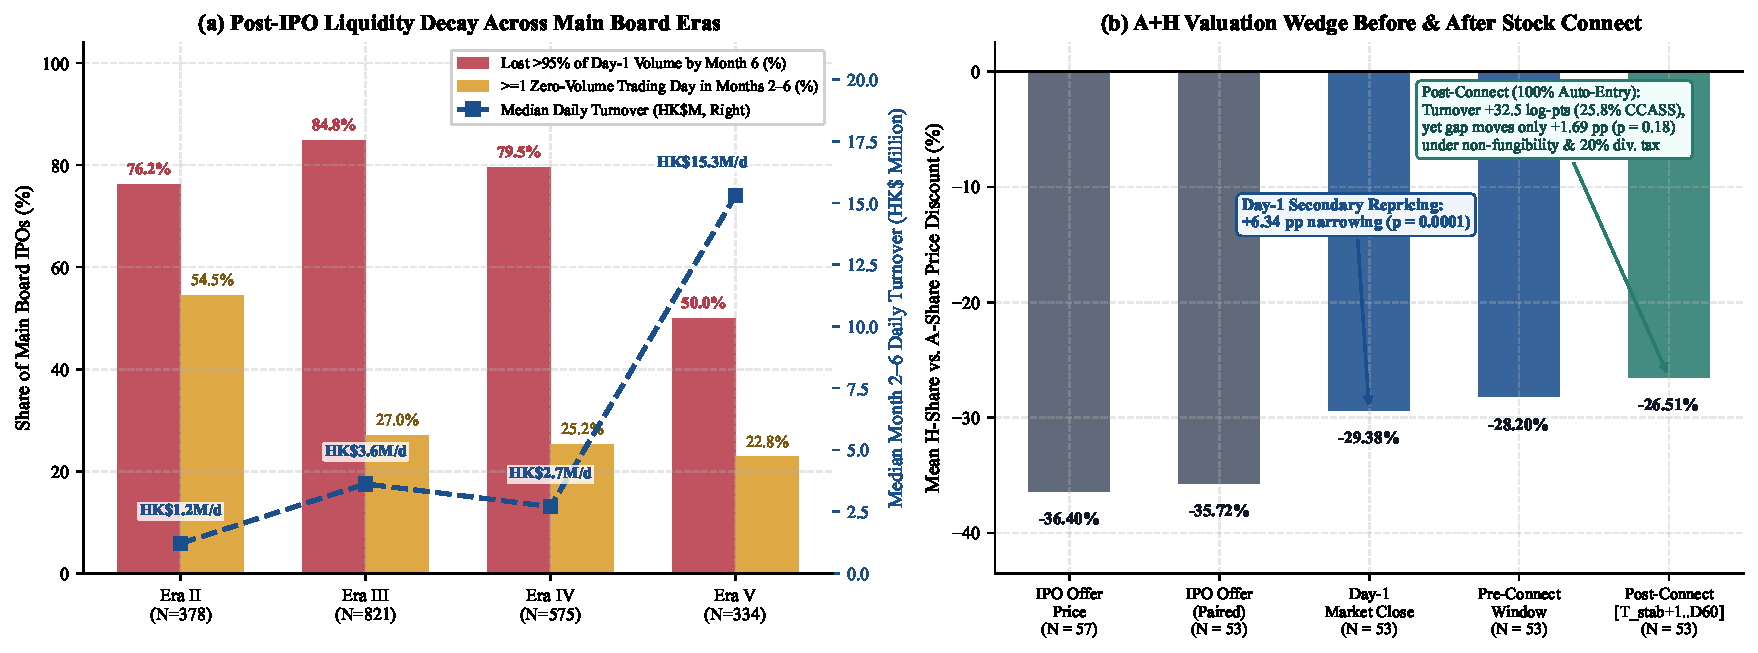
\includegraphics[width=\textwidth,height=0.80\textheight,keepaspectratio]{figures/master_fig8_2_liquidity_and_ah_wedge.pdf}
\caption*{\textbf{Figure 8.3:} Post-IPO liquidity decay across Main Board eras and the persistent A+H valuation wedge before and after Stock Connect. Panel (a) tracks the share of Main Board IPOs losing more than 95\% of Day-1 trading volume by Month 6, zero-volume trading-day incidence in Months 2–6, and median daily trading value across Eras II–V: across Eras II–IV, 76.2\%–84.8\% of Main Board listings lost over 95\% of Day-1 trading volume by Month 6 (with median daily trading value of HK\$1.2M–HK\$3.6M), moderating to 50.0\% and HK\$15.3M/day in Era V. Panel (b) traces mean H-share price discounts relative to onshore A-shares across 2025Q1–2026Q3 A+H offerings from IPO offer price (-36.4\%) through Day-1 close (-29.4\%) and post-stabilization automatic Southbound Connect admission (-26.5\%, an insignificant +1.69 pp post-Connect move despite heavy Southbound trading).}
\end{figure}

Testing whether Southbound Stock Connect genuinely relieves \textbf{investor-base recognition frictions} (Merton, 1987) immediately encounters an acute \textbf{reverse-causality trap}. Non-A+H IPOs admitted to Connect exhibit massive gains in daily trading value relative to excluded peers (+1.52 log points), yet hot stocks cross the HK\$5.0 billion Hang Seng Composite Index (HSCI) market-capitalization gate precisely \textit{because} investor demand already drove up their prices and trading activity. Balance diagnostics confirm that exact selection bias: right at the HK\$5.0 billion threshold, pre-determined Day-1 initial returns jump by more than 90 percentage points alongside surging retail oversubscription, disqualifying naive HSCI cutoff designs (Appendix C.3). To bypass endogenous capitalization sorting, we pivot to a rule-driven institutional contrast: \textbf{A+H dual-listed issuers}, which enter Southbound Connect \textit{automatically} on the trading day after Cap. 571W stabilization ends ($T_{\text{stab}}+1$) regardless of debut returns, versus \textbf{non-A+H Main Board peers} exiting the identical 30-day stabilization window without Connect entry (Figure 8.2b). Controlling for issuer and event-day fixed effects ($N = 219$ issuers), automatic A+H entrants experience a \textbf{36\% relative jump in daily trading value} (+0.307 log points), a lift that holds essentially unchanged at \textbf{34\%} even after ruling out differential Greenshoe unwinds at stabilization expiry. CCASS shareholding records as of November 12, 2026 corroborate the ownership channel directly: Southbound investors hold a mean \textbf{25.8\%} of H-share float in automatic A+H entrants (median 23.7\%, reaching nearly 60\% at the top) versus \textbf{7.4\%} in semi-annual HSCI entrants and zero in excluded non-A+H issues. Even this cleaner design warrants restraint: A+H daily trading value already trends modestly upward in the week before admission, Connect entry coincides by rule with stabilization expiry, and a single CCASS snapshot cannot separate Connect order flow from differential post-stabilization trading trajectories (full event windows, exact stabilization-date subsets, Greenshoe controls, and pre-trend diagnostics appear in Table C.1 and Appendix C.3).

If Southbound order flow reflected true cross-border market integration rather than isolated liquidity plumbing, that sharp expansion in Mainland investor ownership should simultaneously arbitrage away the valuation gap between identical cash-flow claims listed in Shanghai/Shenzhen and Hong Kong. Tracking the A–H price discount across listing stages cleanly tests \textbf{limits to arbitrage under non-fungible capital accounts} (Froot and Dabora, 1999; Jia, Wang, and Xiong, 2017). In recent A+H offerings, H-shares price at an average discount of roughly one-third relative to onshore A-shares (-36.4\% at offer); debut trading narrows the gap modestly (-29.4\% at Day-1 close), yet automatic Connect admission barely compresses it further (-26.5\% post-Connect; Figure 8.3b and Table C.1). Because A- and H-shares cannot be converted across China's closed capital account—preventing arbitrageurs from buying discounted H-shares and shorting identical A-shares onshore—and dividend withholding taxes differ across borders, Stock Connect expands cross-border daily trading value while leaving valuation segmentation firmly intact.

Several evidential caveats bound these aftermarket conclusions. The extreme skewness of lifetime outcomes is a robust long-run fact, whereas negative mean one-year performance is far more sensitive to era, weighting, and factor specification. Offer-price returns are not realized institutional returns, because no dataset here records actual allocations or holding periods, and the lockup, Stock Connect, and A+H results rest largely on recent cohorts whose post-listing windows are still maturing. The gains on offered shares accrue to their owners. To understand what Hong Kong itself gained, we follow the fees, services, and recurring trading activity generated by those listings.

\par\vspace{16pt}\needspace{9\baselineskip}
\noindent\rule{\linewidth}{0.85pt}\par\vspace{5pt}
{\centering\Large\bfseries\color{NavyAccent} \texorpdfstring{PART III — WHAT THE MARKET MADE POSSIBLE}{PART III — WHAT THE MARKET MADE POSSIBLE}\par}
\vspace{4pt}\noindent\rule{\linewidth}{0.85pt}\par\vspace{8pt}
\addcontentsline{toc}{section}{\texorpdfstring{\textbf{PART III — WHAT THE MARKET MADE POSSIBLE}}{PART III — WHAT THE MARKET MADE POSSIBLE}}
Part II showed how the money moves. Part III asks what it left behind. Who benefited in Hong Kong itself? What became of the Mainland companies that came to market? Whose capital was involved, and what would have happened if the bridge had not existed?

\par\medskip\noindent\rule{\linewidth}{0.35pt}\par\medskip
\section*{\texorpdfstring{Section 9. What the IPO Market Built in Hong Kong}{Section 9. What the IPO Market Built in Hong Kong}}
\addcontentsline{toc}{section}{\texorpdfstring{Section 9. What the IPO Market Built in Hong Kong}{Section 9. What the IPO Market Built in Hong Kong}}
\markright{Section 9. What the IPO Market Built in Hong Kong}
Most of the capital raised in Hong Kong IPOs passes through the city to finance corporate operations elsewhere. What remains in Hong Kong is the economic activity surrounding the security: legal, accounting, and advisory work at the time of issuance, followed by decades of secondary trading, clearing, data, and follow-on corporate finance. Within HKEX's own income statement, recurring trading and post-trade revenues dwarf listing fees, while for local households the most memorable primary-market milestones were not ordinary corporate IPOs at all, but public-asset sales such as the Tracker Fund, MTR, and Link REIT.

\subsection*{\texorpdfstring{9.1 Following a Dollar: What Counts as Hong Kong's Gain?}{9.1 Following a Dollar: What Counts as Hong Kong's Gain?}}
\addcontentsline{toc}{subsection}{\texorpdfstring{9.1 Following a Dollar: What Counts as Hong Kong's Gain?}{9.1 Following a Dollar: What Counts as Hong Kong's Gain?}}
The first step is to avoid counting the wrong thing. IPO proceeds are not Hong Kong output. When global investors buy CATL shares to fund a plant in Hungary, the money passes through Hong Kong, but only the value added by resident producers enters local GDP. Fees count only to the extent that they are earned and produced here. Capital gains belong to shareholders wherever they live, and they add to Hong Kong household wealth only for local residents. Financial services as a whole account for roughly a quarter of GDP, but that sector is dominated by banking, insurance, and asset management, so it is context and not a measure of the IPO effect.

Following a single Hong Kong dollar raised at IPO (Figure 9.1) connects primary capital formation to the one-off services and recurring market activity that stay behind. First, nearly all of each dollar with a verified structure—about 94 cents—goes to the issuer as new equity capital, while a small remainder goes to selling shareholders (Section 5.1). Second, a few cents pay for deal-time services at listing: about four cents on a dollar-weighted basis, though far more for a smaller issuer (Section 5.3). Third, most net proceeds depart for factories, research pipelines, or bank balance sheets outside Hong Kong—leaving behind the listed security and the multi-decade stream of secondary trading, clearing, advisory, and follow-on corporate finance it sustains.

\begin{figure}[htbp]
\centering
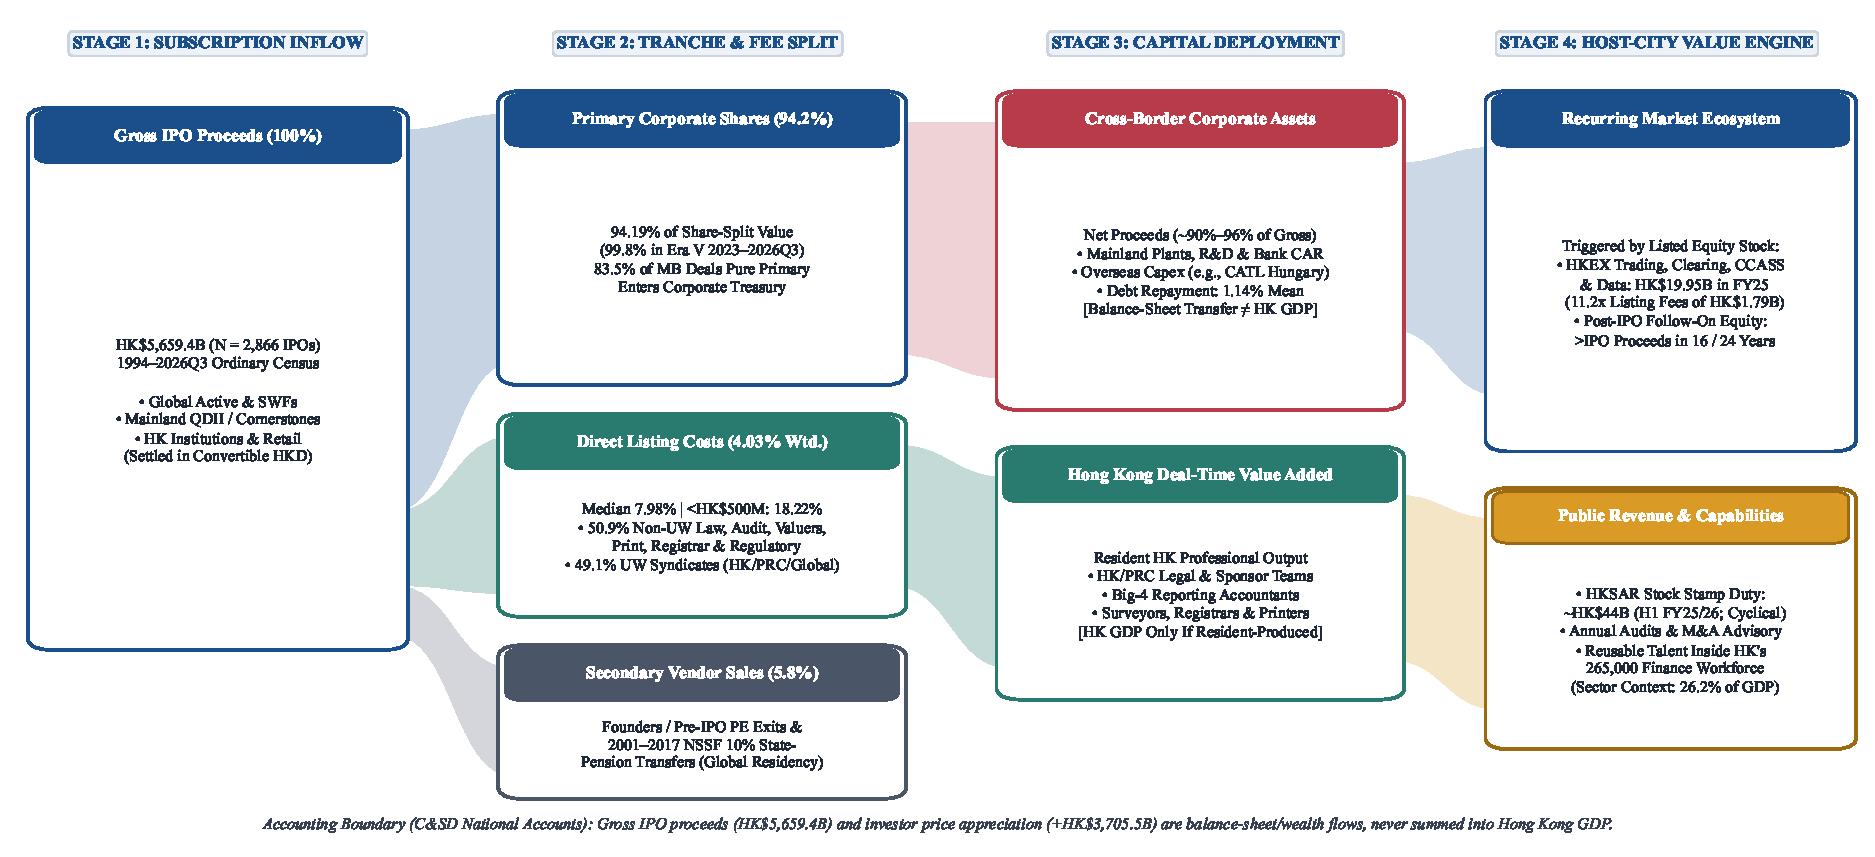
\includegraphics[width=\textwidth,height=0.80\textheight,keepaspectratio]{figures/master_fig9_1_dollar_flow_map.pdf}
\caption*{\textbf{Figure 9.1:} A Dollar Raised in Hong Kong: Capital-Flow and Residency Accounting Map (1994–2026Q3). Moves across four explicit denominators to separate cross-border corporate financing from host-city value added: (1) full 1994–2026Q3 ordinary census gross proceeds ($N = 2,866$, HK\$5,659.4B); (2) share-structure-verified subset ($N = 1,862$, HK\$3,428.4B verified gross proceeds, splitting 94.19\% primary new corporate shares vs. 5.81\% secondary vendor sales); (3) 2025Q1–2026Q3 complete fee-schedule sample ($N = 216$, HK\$24.08B total direct listing expenses on HK\$597.64B gross proceeds = 4.03\% dollar-weighted, of which 50.9\% is non-underwriting services); and (4) exchange-wide recurring host-city activity (Hong Kong Exchanges and Clearing, HKEX, Group FY2025 trading/clearing/custody/data revenue of HK\$19.95B = 11.2$\times$ listing fees, follow-on equity across 24 benchmark years, and HKSAR stamp duty). \textit{Residency boundary}: recipient residency is directly observed only for HKEX Group revenues and HKSAR stamp duty; prospectus fee schedules record service type rather than where legal/audit/underwriting work was produced, and shareholder residency for primary allocations and capital gains is unobserved in census filings.}
\end{figure}

\subsection*{\texorpdfstring{9.2 Four Channels of Local Value}{9.2 Four Channels of Local Value}}
\addcontentsline{toc}{subsection}{\texorpdfstring{9.2 Four Channels of Local Value}{9.2 Four Channels of Local Value}}
\textbf{Deal-time services.} In the 216 recent IPOs with complete expense and commission schedules (the full disclosed set corresponding to Table 5.3 plus the one micro-cap outlier trimmed from equal-weighted quartile averages), listing expenses total HK\$24.08 billion on HK\$597.64 billion of gross proceeds, or 4.03\% on a dollar-weighted basis. Roughly half of those expenses (50.9\%, or HK\$12.27 billion) go to non-underwriting services: lawyers, accountants, internal-control advisers, valuers, printers, registrars, and regulators. On small deals this share is close to four-fifths, and on the largest it is about one-third. We should be careful with the implication. Those payments are not all earned in Hong Kong, since Mainland and international counsel, industry consultants, and offshore offices are in the mix. Underwriting fees, conversely, may be partly earned by Hong Kong staff. Prospectuses show what kind of service was bought, but not where the value was produced. So ``half the bill'' is the amount exposed to local professional services, and Hong Kong's actual retained share remains to be measured.

\begin{figure}[htbp]
\centering
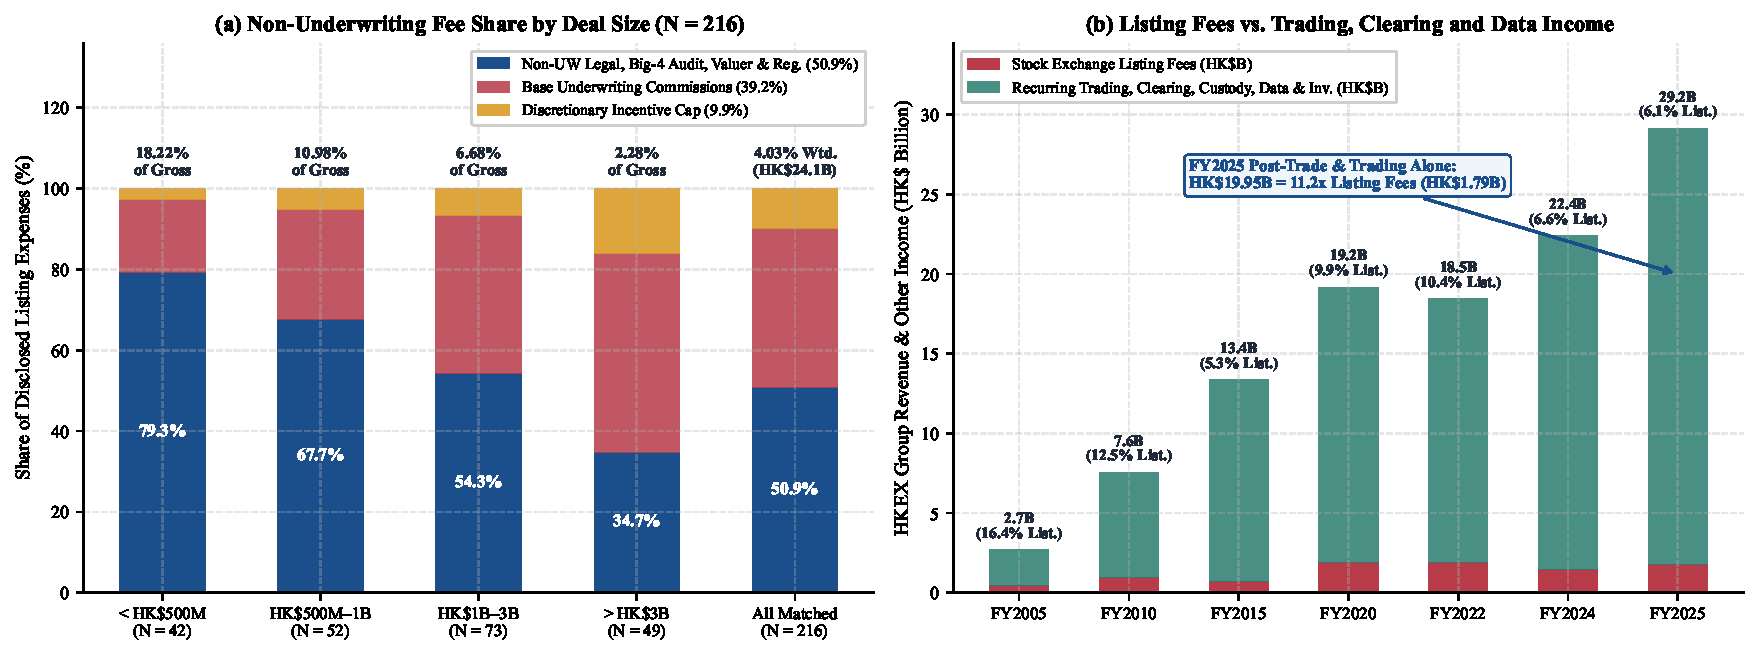
\includegraphics[width=\textwidth,height=0.80\textheight,keepaspectratio]{figures/master_fig9_2_fees_and_hkex_revenue.pdf}
\caption*{\textbf{Figure 9.2:} Non-underwriting fee shares across deal-size tiers and two decades of recurring Hong Kong Exchanges and Clearing (HKEX) Group revenue structure. Panel (a) decomposes HK\$24.08 billion of disclosed listing expenses across all $N = 216$ complete 2025Q1–2026Q3 Main Board fee schedules (including the micro-cap outlier trimmed from Table 5.3's equal-weighted quartiles), showing that non-underwriting legal, audit, and advisory services absorb 50.9\% (HK\$12.27B) overall—ranging from 79.3\% on offerings below HK\$500M down to 34.7\% above HK\$3B. Panel (b) compares Stock Exchange listing fees (initial plus annual) against trading, clearing, custody, market-data, and investment income across FY2005–FY2025 (HKEX Annual Reports), showing that HKEX is overwhelmingly a post-listing annuity rather than an IPO listing-fee business: total group revenue grew more than tenfold from HK\$2.69B (FY2005) to HK\$29.16B (FY2025), while listing fees shrank to 6.1\% (HK\$1.79B) and recurring trading, clearing, custody, and data lines reached HK\$19.95B (11.2$\times$ listing fees).}
\end{figure}

\textbf{The asset-side engine and recurring exchange business.} Accounting strictly for direct fees still misses the deeper economic reason why the stock market made modern Hong Kong into a global financial center. In financial economics, an offshore hub cannot live on settlement plumbing alone; it requires a continuous supply of investable, priceable assets that global and regional portfolios actually want to hold. Primary IPOs, paired with the follow-on placements documented in Section 5.4, serve as Hong Kong's \textbf{asset-side supply engine}. By converting Mainland corporate cash flows into Common Law, U.S.-dollar-pegged equities, each listing feeds a multi-decade urban flywheel: it supplies the underlying securities that sustain secondary trading value, derivatives and structured-product hedging, custodian and margin-lending balances, asset- and wealth-management mandates (SFC AWMAS), and offshore Hong Kong-dollar liquidity demand under the currency board. HKEX's own income statement illustrates this annuity structure: listing fees, which combine initial charges with annual fees paid by listed companies, have fallen to about 6\% of group revenue, whereas trading, clearing, depository, and market-data income was 11.2 times listing fees in FY2025. Although group totals also include derivatives and the London Metal Exchange and cannot be attributed to IPOs alone, the exchange and its surrounding financial cluster clearly earn most of their return after Day 1.

Public finance follows the same rhythm. Hong Kong taxes neither capital gains nor dividends, so government revenue from the stock market comes largely through stamp duty on transfers. Total stamp duty, which also includes property, rose to about HK\$100 billion in 2021–22, fell to about HK\$49 billion in 2023–24, and recovered to about HK\$64 billion in 2024–25. The fiscal link runs through secondary-market activity and not through the amount raised in IPOs.

\textbf{People and capabilities.} Thirty years of cross-border offerings also trained lawyers, accountants, compliance officers, and regulators who understand both Mainland business and Common Law expectations. These skills transfer to follow-on deals, restructurings, acquisitions, and wealth management. They are real, though harder to measure than fees.

\textbf{Distributional incidence.} Those local gains are unevenly shared. High-paying financial and professional jobs are concentrated among a mobile elite, small local firms face entry costs that can reach nearly a fifth of proceeds raised, and while ordinary savers can capture modest gains from one-lot applications (Section 7.4), the median long-run IPO outcome remains deeply negative (Section 8.2).

\begin{calloutbox}{NavyAccent}{Research Note}
\textbf{Box 9.1 — When the Public Became the Investor: Public-Asset Listings (1999–2005).} For ordinary Hong Kong households, the defining primary-market milestones were not corporate capital raises but three public-asset sales (full terms in Appendix B, Table B.1). \textbf{Tracker Fund of Hong Kong (2800.HK, Nov 1999; off-census ETF)} unwound the government's HK\$118 billion August 1998 market-defense portfolio via a HK\$33.3 billion initial offering attracting over 180,000 retail buyers through a 5.25\% discount and loyalty bonus units, turning emergency intervention into a mass index-savings product. \textbf{MTR Corporation (0066.HK, Oct 2000; in-census government secondary sale)} distributed 3.4 million application forms (\textasciitilde{}600,000 retail applicants) for 1.0 billion shares at up to HK\$9.38, making popular shareholding visible while locking the railway into a permanent balancing act between minority dividends and public-transit fare obligations. \textbf{Link REIT (0823.HK, Nov 2005; off-census REIT)} divested HK\$33.8 billion of Housing Authority estate malls and carparks (HK\$22B–23.7B raised) after a tenant judicial review delayed its 2004 debut; strong long-run unitholder returns sat alongside persistent resident conflict over commercial rent hikes and neighborhood-shop displacement, a reminder that fiscal monetization, investor return, and local resident welfare do not automatically align.
\end{calloutbox}

These host-city channels are well documented, though key measurement gaps remain. Fee composition is observable for recent deals and HKEX revenue is audited, yet the geographic residency of fee income, local employment caused by IPOs, and Hong Kong household capital gains are not directly observed. Quantifying the exact share of value retained within the city therefore remains an open empirical problem. Having traced what stayed in Hong Kong, we now follow the primary proceeds across the border into Mainland enterprises.

\par\medskip\noindent\rule{\linewidth}{0.35pt}\par\medskip
\section*{\texorpdfstring{Section 10. Financing China's Corporate Transformation}{Section 10. Financing China's Corporate Transformation}}
\addcontentsline{toc}{section}{\texorpdfstring{Section 10. Financing China's Corporate Transformation}{Section 10. Financing China's Corporate Transformation}}
\markright{Section 10. Financing China's Corporate Transfo...}
What did listing in Hong Kong change inside Mainland companies—both in corporate governance before the debut and in how firms deployed initial proceeds and subsequent follow-on equity (Section 5.4)? For state enterprises in the 1990s, the most important change came before the first share was sold. For later firms the answer varies widely, from a recapitalized bank returning for rights issues to a technology company that never tapped follow-on public equity at all.

\subsection*{\texorpdfstring{10.1 Reorganizing the State Enterprise}{10.1 Reorganizing the State Enterprise}}
\addcontentsline{toc}{subsection}{\texorpdfstring{10.1 Reorganizing the State Enterprise}{10.1 Reorganizing the State Enterprise}}
In the early 1990s, a Chinese state factory could be a production unit, landlord, school operator, clinic, and pension provider all at once. To list in Hong Kong it had to become something outsiders could value. Commercial assets were carved into a joint-stock company, social functions stayed behind with the parent, accounts were restated under international standards, independent directors were appointed, and minority protections were written into corporate charters (Cha, 2023). Research on China's share-issue privatization finds measurable improvements in disclosure and operating performance, yet also documents the structural limits of partial privatization when state ownership and politically connected executives remain entrenched (Sun and Tong, 2003; Fan, Wong, and Zhang, 2007; Jiang, Yue, and Zhao, 2009). At the same time, onshore listing decisions in China have historically been intertwined with local political promotion cycles and administrative quotas (Piotroski and Zhang, 2014; Qian, Ritter, and Shao, 2024). Hong Kong's market-oriented timetable therefore offered two distinct governance services: for state enterprises, it supplied an external reporting and valuation anchor that domestic restructuring alone could not replicate; for private growth firms, it provided an exit from administrative rationing and politically correlated onshore queues.

The large banks need especially careful attribution. Did Hong Kong IPOs rescue China's banking system? Not by themselves (IMF, 2006; Bank of China, 2008). The sequence had five parts: sovereign capital injections, asset-management-company disposal of non-performing loans, joint-stock conversion with foreign strategic investors, H-share offerings supplying a market price, disclosure discipline, and hard-currency equity, and subsequent rights issues replenishing Basel capital. The IPO was a late and essential stage in a state-led balance-sheet repair rather than a standalone cure.

\subsection*{\texorpdfstring{10.2 From Offering Proceeds to Real Activity: Four Corporate-Finance Functions}{10.2 From Offering Proceeds to Real Activity: Four Corporate-Finance Functions}}
\addcontentsline{toc}{subsection}{\texorpdfstring{10.2 From Offering Proceeds to Real Activity: Four Corporate-Finance Functions}{10.2 From Offering Proceeds to Real Activity: Four Corporate-Finance Functions}}
What happens after the money arrives? Aggregate statistics cannot trace capital inside the firm, so Table 10.1 follows five archetypal issuers—three cross-era corporate-finance benchmarks plus an explicitly matched pair of inaugural Chapter 18A biotechs—using a common six-question protocol: pre-IPO constraint, primary structure, stated use of proceeds, post-IPO follow-on behavior, real operational outcome, and attribution limit. Taken together, these histories illustrate \textbf{four distinct cross-system functions} that Hong Kong performed for China's corporate sector, while the counterexamples demonstrate that public markets price plans rather than guarantee execution.

\begin{table}[!htbp]
\centering
\caption*{Table 10.1 — From Proceeds to Operations: Five Archetypal Issuer Case Histories and a Matched Chapter 18A Pair (6-Question Protocol)}
\begin{adjustbox}{max width=\textwidth,max totalheight=0.79\textheight}
\begin{minipage}{\textwidth}\centering
\footnotesize
\setlength{\tabcolsep}{3.5pt}
\renewcommand{\arraystretch}{1.18}
\begin{adjustbox}{max width=\textwidth}
\begin{tabular}{>{\raggedright\arraybackslash}p{2.26cm}>{\raggedright\arraybackslash}p{2.71cm}>{\raggedright\arraybackslash}p{2.71cm}>{\raggedright\arraybackslash}p{2.71cm}>{\raggedright\arraybackslash}p{2.71cm}>{\raggedright\arraybackslash}p{2.71cm}}
\toprule
Dimension & 1. State Bank Recapitalization: \textbf{ICBC (1398.HK, Oct 2006)} & 2. Private Tech Compounder: \textbf{Tencent (0700.HK, Jun 2004)} & 3. Outbound Industrial Globalizer: \textbf{CATL (3750.HK, May 2025)} & 4. Ch. 18A Biotech Scaler: \textbf{Innovent (1801.HK, Oct 2018)} & 5. Ch. 18A Reversal Foil: \textbf{Ascletis (1672.HK, Aug 2018)} \\
\midrule
\textbf{1. Pre-IPO Constraint} & Post-1990s NPL legacy \& thin Basel capital adequacy & Cayman/VIE internet firm barred from onshore A-shares & Already Shenzhen-listed (RMB 270.2B cash), needing \textbf{offshore EUR/USD} insulated from FX controls & Zero commercial revenue (HK\$4.04M Y-1); barred by pre-2018 profit gates & Pre-profit Mainland antiviral biotech; barred by pre-2018 profit gates \\
\textbf{2. Primary Split \& Terms} \textit{(Census Verified)} & Ch. 19A A+H; \textbf{HK\$3.07}; \textbf{HK\$124.95B} HK gross; 2.50\% spread; +14.66\% Day-1; +37.73\% 1Y BHAR & \textbf{100\% pure primary} (0 sale shares); \textbf{HK\$3.70}; \textbf{HK\$1.788B} gross (HK\$1,454M net); +12.16\% Day-1; +29.63\% 1Y BHAR & Ch. 19A A+H \textbf{100\% primary}; \textbf{HK\$263.00}; \textbf{HK\$41.01B} gross (HK\$40.63B net); \textbf{0.20\% base UW / 0.81\% total}; +12.39\% Day-1; +108.04\% 1Y BHAR & Early \textbf{Ch. 18A}; \textbf{HK\$13.98}; \textbf{HK\$3.80B} gross; 3.0\% spread; +18.60\% Day-1; +36.44\% 1Y BHAR & Inaugural \textbf{Ch. 18A}; \textbf{HK\$14.00}; \textbf{HK\$3.14B} gross; 2.5\% spread; 0\% CS; 0.00\% Day-1; \textbf{-67.03\% 1Y BHAR} (-63.48\% BHR) \\
\textbf{3. Prospectus Use of Proceeds} & Strengthen core Tier-1 capital base and \textbf{CAR} & Open-ended strategic mandate (\textit{messaging, R\&D, M\&A}) & \textbf{\textasciitilde{}90\% earmarked for Debrecen, Hungary EV-battery Phases I \& II} (pp. 310–311) & Phase II/III clinical trials (\textit{sintilimab}), Suzhou GMP plant, R\&D & Antiviral (HCV) clinical R\&D, commercialization \& pipeline expansion \\
\textbf{4. Post-IPO Utilization \& Follow-On} & Immediately fortified CAR; returned for \textbf{2010 A+H rights issue} for Basel III & \textbf{Zero follow-on equity in 22+ years}; funded growth via cash flow \& \textbf{2014+ GMTN bonds} & \textbf{2025 Annual Report}: disbursing on schedule into Hungary plant \& equipment; zero follow-on & Repeated \textbf{general-mandate top-up placings} (2019–2025, incl. HK\$4.31B Jun 2025) + pharma out-licensing & Core hepatitis-C commercial rollout stalled after NRDL reimbursement shifts; pipeline reprioritized \\
\textbf{5. Real Operational Outcome} & Scaled into world’s largest listed bank under IFRS \& quarterly reporting & Scaled QQ/WeChat ecosystem; \textbf{+HK\$1,093.2B} offered-tranche gain (\textbf{29.5\%} of market total) & FY 2025 revenue +17\% to RMB 423.7B, profit RMB 72.2B (\textasciitilde{}96.9\% utilization) & Commercialized PD-1 \& GLP-1 assets; \textbf{\textgreater{}RMB 10B revenue \& first full-year profit in FY 2025} & FY 2025 product revenue just \textbf{RMB 2.03M} amid \textbf{RMB 300M+} annual losses; severe repricing \\
\textbf{6. Attribution Limit} & Huijin / AMC / strategic investors fixed solvency pre-IPO; HK gave benchmark \& rights access & HKEX did \textit{not} fund 20Y R\&D from HK\$1.45B; Cayman-VIE rule gave early liquidity \& debt access & HKEX did \textit{not} create CATL tech; it supplied \textbf{fast hard-currency EUR/USD capex syndication} & Right-tail 18A survivor; depended equally on clinical trials \& NRDL reimbursement & IPO gates price promise, not execution—mirrored in Shinsun 2599.HK \& international peer Razer 1337.HK \\
\bottomrule
\end{tabular}
\end{adjustbox}
\end{minipage}
\end{adjustbox}
\par\vspace{3pt}\noindent\parbox{\textwidth}{\scriptsize\raggedright \textit{Notes}: \textit{Selection and matching design}: Columns 1–3 trace three distinct cross-era corporate-finance archetypes (state-bank recapitalization, private technology compounding, and outbound A+H industrial expansion), whereas Columns 4 and 5 form an explicit \textbf{within-track matched pair} of inaugural 2018 Chapter 18A pre-revenue biotech listings—matched on listing route, cohort timing (two months apart), offer price (HK\$13.98 vs. HK\$14.00), and deal scale (HK\$3.80B vs. HK\$3.14B)—that diverged sharply after listing (+36.44\% vs. -67.03\% 1Y BHAR; \textgreater{}RMB 10B vs. RMB 2.03M FY2025 revenue), illustrating that listing gates price plans rather than guarantee commercial execution. \textit{Source}: 33-year census, 2025–2026Q3 panel, IPO prospectuses of the five featured issuers (ICBC October 2006, Tencent June 2004, CATL May 2025, Innovent October 2018, and Ascletis August 2018), and subsequent annual reports (with secondary reversal comparators Shinsun 2599.HK and Razer 1337.HK noted in Row 6 from their respective listing and privatization filings). Abbreviations: \textit{NPL} = non-performing loan; \textit{VIE} = Variable Interest Entity; \textit{UW} = underwriting; \textit{CS} = cornerstone; \textit{BHAR / BHR} = 1-year buy-and-hold abnormal / raw return; \textit{CAR} = capital adequacy ratio; \textit{GMTN} = Global Medium-Term Note; \textit{GMP} = Good Manufacturing Practice; \textit{NRDL} = National Reimbursement Drug List; \textit{IFRS} = International Financial Reporting Standards; \textit{AMC} = asset management company; \textit{HKEX} = Hong Kong Exchanges and Clearing.}
\end{table}

These five trajectories clarify four distinct corporate-finance functions that Hong Kong performed across China's corporate evolution, illustrating at the firm level the continuing follow-on equity option documented in Section 5.4. In state-bank recapitalization, \textbf{ICBC (2006)} arrived only after sovereign capital injections, bad-loan carve-outs, and foreign strategic investments had repaired core solvency; its Hong Kong offering supplied international market discipline, hard-currency Tier-1 equity, and continuing rights-issue capacity (used in 2010 for Basel III) rather than a standalone bailout. In private technology compounding, \textbf{Tencent (2004)} raised less than HK\$2 billion and funded two decades of expansion from internal cash flow and bond markets without ever returning for follow-on equity, using its Cayman-VIE listing primarily for legal legitimacy, employee-incentive currency, and global credit access—yet generating +HK\$1,093.2 billion in offered-tranche appreciation.

By contrast, \textbf{CATL (2025)} demonstrates Hong Kong's modern \textbf{outbound industrial} role: already cash-rich in Shenzhen, the battery maker listed in Hong Kong primarily to syndicate HK\$40.63 billion in convertible offshore equity earmarked for its Debrecen, Hungary plant. Finally, the Chapter 18A pair illustrates staged risk financing: \textbf{Innovent (2018)} tapped repeated post-IPO top-up placings (Section 5.4) alongside clinical milestones and pharma out-licensing to scale past RMB 10 billion in revenue by FY 2025, whereas \textbf{Ascletis (2018)}—alongside post-listing reversals at Shinsun and Razer—confirms that IPO gates price a business plan rather than guarantee commercial execution. Without a matched control group of comparable unlisted Mainland firms, however, case histories can establish corporate mechanisms rather than causal magnitudes; estimating how much investment, innovation, or productivity listing itself causes remains the central unanswered real-economy question in this field.

\par\medskip\noindent\rule{\linewidth}{0.35pt}\par\medskip
\section*{\texorpdfstring{Section 11. Global Capital: Who Was on the Other Side?}{Section 11. Global Capital: Who Was on the Other Side?}}
\addcontentsline{toc}{section}{\texorpdfstring{Section 11. Global Capital: Who Was on the Other Side?}{Section 11. Global Capital: Who Was on the Other Side?}}
\markright{Section 11. Global Capital}
Although Mainland banks now dominate the sell side of Hong Kong IPOs, it does not follow that Mainland investors supply all of the demand. On the most direct question—who ultimately buys primary IPO allocations—public microdata remain incomplete, requiring careful separation between disclosed primary cornerstone placements, secondary-market trading surveys, and aggregate asset-management pools.

\subsection*{\texorpdfstring{11.1 Who Finances Hong Kong's IPOs?}{11.1 Who Finances Hong Kong's IPOs?}}
\addcontentsline{toc}{subsection}{\texorpdfstring{11.1 Who Finances Hong Kong's IPOs?}{11.1 Who Finances Hong Kong's IPOs?}}
Public records identify buyers through three distinct lenses that measure different slices of market demand and should not be conflated. Closest to the primary market are \textbf{disclosed cornerstone placements} in prospectuses and allotment notices (Table 6.2). They name pre-committed institutional buyers, showing active repeat Mainland insurers, fund managers, and bank wealth units participating alongside global sovereign wealth funds and long-only managers, while leaving unallocated bookbuilt tranches unobserved. Second, \textbf{secondary-market trading data}, specifically HKEX's Cash Market Transaction Surveys (CMTS) through 2020 and post-2020 Southbound Stock Connect daily trading value, measure who trades listed shares after the debut rather than who subscribed at the offer price. Third, the SFC's \textbf{Asset and Wealth Management Activities Survey (AWMAS)} tracks capital managed in Hong Kong by investor origin, even though assets domiciled or managed locally need not be invested in Hong Kong IPOs.

\begin{figure}[htbp]
\centering
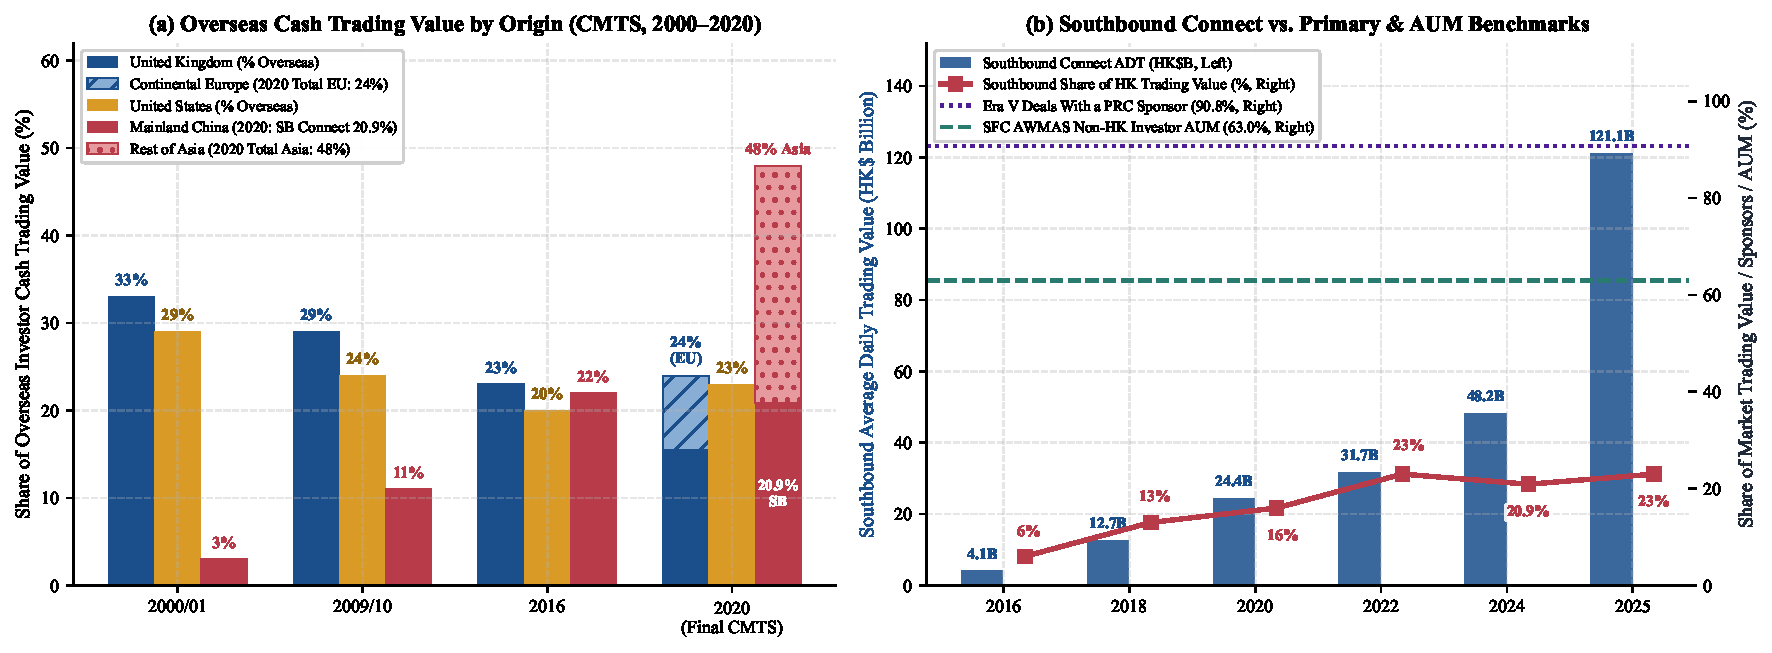
\includegraphics[width=\textwidth,height=0.80\textheight,keepaspectratio]{figures/master_fig11_1_investor_origin_connect.pdf}
\caption*{\textbf{Figure 11.1:} Demand-side investor origin, Southbound Connect daily trading value, and non-Hong Kong asset-management assets under management (AUM) versus primary syndicate composition, 2000–2025. \textit{Takeaway}: juxtaposing sell-side sponsor share against secondary trading flows and locally managed assets shows that Mainland dominance on underwriting teams (90.8\% of Era V deals carry a People's Republic of China, PRC, sponsor) does \textbf{not} imply an exclusively Mainland investor base—Southbound Connect accounts for 23\% of total HKEX cash-market trading value while non-Hong Kong regional and global capital still supplies 63.0\% of Hong Kong AUM and roughly half of overseas cash trading (though direct primary IPO allocation residency remains unobserved outside named cornerstones). Panel (a) disaggregates Hong Kong Exchanges and Clearing (HKEX) Cash Market Transaction Survey (CMTS) shares across 2000/01–2020 using \textbf{overseas investor cash-market trading value} (\textasciitilde{}40\% of total HKEX cash-market trading value; 41.2\% in 2020) as the denominator: U.K. and U.S. shares fell from 62\% combined (2000/01) while Mainland China rose from 3\% to 20.9\% via Southbound Connect (total Asia 48\%, Europe 24\%, U.S. 23\% in 2020). Panel (b) compares three distinct denominators: Southbound Connect average daily trading value (ADT, left axis, HK\$B, scaling fivefold from HK\$24.4B in 2020 to HK\$121.1B in 2025) and Southbound share of \textbf{total HKEX cash-market trading value} (rising from 6\% in 2016 to 23\% in 2025, right axis), against the Securities and Futures Commission (SFC) Asset and Wealth Management Activities Survey (AWMAS) non-Hong Kong investor share of \textbf{total Hong Kong AUM} (63.0\%) and PRC sponsor participation share of \textbf{Era V Main Board IPO deals} (90.8\%).}
\end{figure}

Read together with those boundaries intact, the three series rebut the simple claim that Mainland sponsors imply an exclusively Mainland investor base (Figure 11.1). Across HKEX's cash-market surveys through 2020, the total overseas share of secondary trading value stayed near two-fifths while its geographic composition shifted markedly: in 2000/01, the U.K. and the U.S. supplied most overseas trading and Mainland China hardly registered, whereas by 2020 Mainland investors via Connect had become one of the largest sources and Asia as a whole roughly matched Europe and the U.S. combined. After 2020, Southbound daily trading value grew about fivefold, while Hong Kong's asset-management pool reached a record in 2025 with the majority of assets sourced from outside the city. A dollar-weighted classification of disclosed cornerstone investors by ultimate capital source is feasible and would improve directly on what secondary surveys and aggregate AUM can show.

\subsection*{\texorpdfstring{11.2 What Global Portfolios, U.S. Markets, and Issuers Received}{11.2 What Global Portfolios, U.S. Markets, and Issuers Received}}
\addcontentsline{toc}{subsection}{\texorpdfstring{11.2 What Global Portfolios, U.S. Markets, and Issuers Received}{11.2 What Global Portfolios, U.S. Markets, and Issuers Received}}
For international investors, Hong Kong solved a global portfolio-allocation problem. Over three decades in which China rose from a peripheral economy to the world's second-largest, onshore A-shares remained constrained by capital controls, quota regimes, and unfamiliar legal enforcement. Hong Kong offered a convertible, Common Law gateway into that growth, and the sector mix tracked China's macroeconomic transformation: first infrastructure, energy, and state banking; then consumer internet platforms; then pre-revenue biotechnology; and most recently advanced manufacturing and clean technology. Equally important for global capital-market architecture, Hong Kong acted as a competitive counterweight and geopolitical pressure valve alongside New York. When U.S. securities law (Sarbanes-Oxley in 2002) and later geopolitical audit disputes (HFCAA after 2020) raised the cost of New York listings for Chinese firms, Hong Kong's 2018 Chapter 8A/18A/19C overhaul and 2023–2026 A+H corridor absorbed cross-border capital flows that might otherwise have fractured entirely. Even as Rule 144A U.S. QIB participation in HK\$1B+ offerings retreated from 62.0\% in Era IV to 40.8\% in Era V, global institutional capital did not disappear; instead, bookbuilding rebalanced toward European, Middle Eastern sovereign, pan-Asian, and Southbound Mainland pools.

The poor median IPO return does not imply that institutional allocations were irrational. Large global institutions hold bigger and more liquid firms, and as Section 8.1 demonstrated, IPO-proceeds-weighted Main Board calendar-time returns are indistinguishable from zero once local risk factors (especially book-to-market) are included. Access does not guarantee excess return (Section 8.2), but Hong Kong supplied liquid exposure to an economy that global benchmarks could not ignore.

Issuers gained parallel global benefits beyond cash proceeds: internationally recognized equity for cross-border acquisitions and employee stock incentives, IFRS reporting that reassured overseas customers and supply-chain partners, and lower-cost entry into Eurobond and U.S.-dollar credit markets. These motives explain why cash-rich firms such as Tencent (2004) and CATL (2025) valued a Hong Kong listing even when they had little need for domestic renminbi financing.

\subsection*{\texorpdfstring{11.3 Why Global Brands Came, and Why Many Drifted Away}{11.3 Why Global Brands Came, and Why Many Drifted Away}}
\addcontentsline{toc}{subsection}{\texorpdfstring{11.3 Why Global Brands Came, and Why Many Drifted Away}{11.3 Why Global Brands Came, and Why Many Drifted Away}}
Hong Kong gave global investors access to Chinese companies. Seeing three decades of successful cross-border issuance, however, one might attribute Hong Kong's liquidity purely to generic offshore institutional infrastructure (Common Law courts, a convertible currency, and low taxes) rather than proximity to Greater China cash flows and investor clienteles. The 37 census IPOs from outside Greater China and the usual offshore jurisdictions serve as a natural falsification test of that generic-plumbing hypothesis: if portable legal and currency infrastructure alone sufficed to anchor secondary trading, non-Mainland global consumer and resource brands courted around 2010, including Glencore, Prada, Samsonite, and L'Occitane, should have sustained active Hong Kong order books just as readily as Chinese issuers.

\begin{table}[!htbp]
\centering
\caption*{Table 11.1 — Landmark Non-Greater-China International Listings in Hong Kong: Thesis vs. Post-Listing Outcome}
\begin{adjustbox}{max width=\textwidth,max totalheight=0.79\textheight}
\begin{minipage}{\textwidth}\centering
\footnotesize
\setlength{\tabcolsep}{3.5pt}
\renewcommand{\arraystretch}{1.18}
\begin{adjustbox}{max width=\textwidth}
\begin{tabular}{>{\raggedright\arraybackslash}p{2.46cm}>{\centering\arraybackslash}p{1.90cm}ccc>{\raggedright\arraybackslash}p{3.88cm}>{\raggedright\arraybackslash}p{3.88cm}}
\toprule
Company (Ticker) & Listing Date \& Domicile & Census Gross (HK\$B) & Day-1 IR (\%) & 1Y BHAR (\%) & Original Listing Thesis & Post-Listing Liquidity \& Corporate Outcome \\
\midrule
\textbf{Standard Chartered (2888.HK)} & Oct 2002 (GB) & 2.94 & +3.57\% & +13.99\% & Historical Asia/HK banking franchise dual listing & Durable dual listing anchored in HK retail/institutional base \\
\textbf{UC Rusal (0486.HK)} & Jan 2010 (RU) & 17.39 & -10.56\% & +6.35\% & First Russian industrial primary IPO tapping Asian capital & Thin secondary free-float liquidity; geopolitically segmented \\
\textbf{L’Occitane (0973.HK)} & May 2010 (LU/FR) & 6.11 & -4.51\% & +14.16\% & Asian luxury skincare growth \& brand visibility & Valuation discount vs. European peers led founder to \textbf{privatize \& delist (Oct 2024)} \\
\textbf{Glencore (0805.HK)} & May 2011 (JE/CH) & 77.75 \textit{(dual LSE)} & -2.45\% & -16.88\% & Anchor Asian institutional ownership alongside London IPO & \textbf{Voluntarily delisted Jan 2018}: only \textbf{\textasciitilde{}0.3\%} of shares sat on HK register \textit{(code 0805 later recycled in Jan 2025)} \\
\textbf{Samsonite (1910.HK)} & Jun 2011 (LU/US) & 10.09 & -7.72\% & +2.67\% & Asian travel-consumer growth \& PE exit & Persistent liquidity/valuation gap prompted pursuit of \textbf{U.S. dual listing} \\
\textbf{Prada (1913.HK)} & Jun 2011 (IT) & 19.23 & +0.25\% & +40.21\% & Luxury multiples anchored in Greater China demand & Strong early returns, yet repeated reviews of \textbf{Milan dual listing} for EU liquidity \\
\textbf{Coach (6388.HK)} \textit{(Off-Census HDR)} & Dec 2011 (US HDR) & \textit{Intro (HK\$0)} & — & — & First U.S. \textbf{Hong Kong Depositary Receipt} for brand visibility & \textbf{Withdrew its listing} after chronically thin local trading (Appendix B) \\
\textbf{Ferretti (9638.HK)} & Mar 2022 (IT) & 2.01 & -0.13\% & +7.48\% & Italian luxury yacht maker (Weichai-backed) & \textbf{Dual-listed in Milan in 2023} to capture home-market European liquidity \\
\bottomrule
\end{tabular}
\end{adjustbox}
\end{minipage}
\end{adjustbox}
\par\vspace{3pt}\noindent\parbox{\textwidth}{\scriptsize\raggedright \textit{Notes}: \textit{Population and takeaway}: Representative cases drawn from the \textbf{37 ordinary IPOs in the 2,866 census domiciled outside Greater China} (excluding Mainland China, Hong Kong, Macau, and Taiwan issuers as well as Cayman Islands, Bermuda, and British Virgin Islands holding vehicles for Greater China businesses), plus Coach (6388.HK), an off-census U.S. Hong Kong Depositary Receipt (HDR) listing by introduction included as a liquidity comparator. Across these cases, generic offshore legal and currency infrastructure sufficed to secure initial listings, yet issuers without a local operating franchise (Glencore, Coach, L'Occitane, Samsonite, Ferretti) suffered thin local trading and drifted back toward home markets, leaving locally anchored Standard Chartered as the durable exception. \textit{Definitions}: \textit{Day-1 IR} is $(P_1 - P_0)/P_0$; \textit{1Y BHAR} is one-year buy-and-hold abnormal return from Day-1 close $P_1$ over the estimated dividend-reinvested Hang Seng benchmark; \textit{LSE} = London Stock Exchange; \textit{PE} = private equity. \textit{Source}: 33-year ordinary IPO census, Hong Kong Exchanges and Clearing (HKEX) \textit{International Companies Review} (2023), corporate delisting/privatization circulars, and Appendix B Off-Census Ledger.}
\end{table}

Getting listed proved far easier than sustaining an active secondary market. For nearly a decade after Stock Connect's launch, foreign-incorporated primary listings were excluded from Southbound eligibility, cutting them off from Hong Kong's fastest-growing pool of cross-border liquidity; even after HKEX and Mainland regulators expanded Southbound Stock Connect in March 2023 to admit qualifying primary-listed international companies included in the Hang Seng Composite Index, trading in non-Greater-China issuers continued to gravitate back toward home exchanges where analysts, index funds, and corporate headquarters reside (Froot and Dabora, 1999; Karolyi, 2006). Glencore's Hong Kong share register dwindled to roughly 0.3\% before its 2018 delisting, Coach withdrew its depositary receipts after local trading value evaporated, L'Occitane and Razer privatized at discounts, and Samsonite and Ferretti pursued U.S. or Milan listings to recapture home-market multiples. Standard Chartered is the instructive exception precisely because Hong Kong and Greater China form the core of its commercial banking franchise: branding alone can secure a listing, whereas durable liquidity requires local earnings, local investors, or natural inclusion in Mainland-facing benchmarks.

The demand-side record also carries clear evidential limits. Investor-origin data are strongest for secondary trading before 2020 and weakest for recent primary allocations, while the international-issuer analysis rests on a small number of cases and should be read as an institutional comparison.

\par\medskip\noindent\rule{\linewidth}{0.35pt}\par\medskip
\section*{\texorpdfstring{Section 12. Counterfactuals, Trade-offs, and Conclusion}{Section 12. Counterfactuals, Trade-offs, and Conclusion}}
\addcontentsline{toc}{section}{\texorpdfstring{Section 12. Counterfactuals, Trade-offs, and Conclusion}{Section 12. Counterfactuals, Trade-offs, and Conclusion}}
\markright{Section 12. Counterfactuals, Trade-offs, and Co...}
No dataset can directly observe the counterfactual world without Hong Kong's equity bridge. Comparing what contemporary alternatives could offer in each era, however, separates the institutional value Hong Kong genuinely produced from the volume it inherited from restrictions elsewhere.

\subsection*{\texorpdfstring{12.1 Era-by-Era Counterfactuals}{12.1 Era-by-Era Counterfactuals}}
\addcontentsline{toc}{subsection}{\texorpdfstring{12.1 Era-by-Era Counterfactuals}{12.1 Era-by-Era Counterfactuals}}
\begin{table}[!htbp]
\centering
\caption*{Table 12.1 — Era-by-Era Counterfactual Matrix: Hong Kong vs. Contemporary Alternatives (1994–2026)}
\begin{adjustbox}{max width=\textwidth,max totalheight=0.79\textheight}
\begin{minipage}{\textwidth}\centering
\footnotesize
\setlength{\tabcolsep}{3.5pt}
\renewcommand{\arraystretch}{1.18}
\begin{adjustbox}{max width=\textwidth}
\begin{tabular}{l>{\raggedright\arraybackslash}p{2.90cm}>{\raggedright\arraybackslash}p{2.90cm}>{\raggedright\arraybackslash}p{2.90cm}>{\raggedright\arraybackslash}p{2.90cm}>{\raggedright\arraybackslash}p{2.90cm}}
\toprule
Historical Era & Primary Issuer Cohort & Mainland A-Shares (SSE / SZSE) & U.S. Venues (NYSE / Nasdaq) & London / Singapore / Private PE & Marginal Institutional Value Added by Hong Kong \\
\midrule
\textbf{Eras I–II (1994–2007)} & SOE Pioneers \& Mega-Banks (\textit{Tsingtao}, \textit{ICBC}, \textit{BOC}, \textit{Tencent}) & Illiquid, non-tradable state shares; administrative quotas \& frequent IPO freezes (Qian, Ritter, \& Shao, 2024) & Open to select SOEs (\textit{China Life}, \textit{PetroChina}), but \textbf{SOX 2002} \& U.S. litigation raised entry barriers & London captured select resources; Singapore lacked mega-cap depth & \textbf{Hard-currency USD/HKD price discovery, IFRS governance surgery, and Cayman-VIE accommodation} when A-shares could not absorb mega-SOEs or private tech \\
\textbf{Era III (2008–2017)} & Private Growth, Global Brands \& Financials (\textit{AIA}) & \textbf{23x P/E ceiling}, multi-year CSRC queue, and \textbf{2012–13 / 2015 IPO freezes} & Captured \textit{Alibaba (2014)} via \textbf{WVR}, which HKEX then prohibited & Singapore lacked Stock Connect; private PE could not provide public exits at scale & \textbf{Predictable 6–9 month listing timetable, Stock Connect bridge (2014/16), and post-IPO follow-on liquidity (HK\$848B in 2015)} \\
\textbf{Era IV (2018–2022)} & New Economy (Ch. 8A), Pre-Revenue Biotech (Ch. 18A), ADR Homecomings (Ch. 19C) & \textbf{STAR Market (2019)} launched, but profitability/VIE \& FX convertibility limits persisted & \textbf{HFCAA delisting risk} \& U.S.–China tech decoupling chilled New York access & London/Singapore unable to match Greater China biotech/tech investor base & \textbf{Insulated offshore homecoming \& pre-revenue biotech (Ch. 18A) risk-capital ecosystem} \\
\textbf{Era V (2023–2026Q3)} & Outbound Industrial A+H (\textit{CATL}), Hard-Tech (Ch. 18C) & Onshore \textbf{A-share IPO tightening (2023–25)} pushed quality issuers offshore & Geopolitical \& outbound-investment restrictions curtailed U.S. China IPOs & Domestic bank debt abundant in RMB, \textit{not} in convertible EUR/USD offshore capex & \textbf{Fast hard-currency (EUR/USD/HKD) syndication (0.2\% base UW), Reg S global/Middle East/Southbound routing, and T+2 FINI efficiency} \\
\bottomrule
\end{tabular}
\end{adjustbox}
\end{minipage}
\end{adjustbox}
\par\vspace{3pt}\noindent\parbox{\textwidth}{\scriptsize\raggedright \textit{Notes}: \textit{Assessment method}: Rather than estimating a structural counterfactual model, this comparative institutional matrix evaluates contemporary rival venues in each era against Hong Kong Exchanges and Clearing (HKEX) along four documented criteria from Sections 2–11 and Qian, Ritter, and Shao (2024): currency convertibility, entry/governance eligibility (profit gates, dual-class shares, Variable Interest Entities [VIEs], administrative quotas), regulatory and geopolitical market access, and secondary/follow-on liquidity depth. \textit{Takeaway}: Hong Kong's marginal value evolved from mega-SOE absorption and governance restructuring (Eras I–II) to predictable timetables and new-economy/biotech gateways (Eras III–IV) and fast hard-currency EUR/USD syndication (Era V). Abbreviations: \textit{SOE} = state-owned enterprise; \textit{SSE / SZSE} = Shanghai / Shenzhen Stock Exchanges; \textit{SOX} = U.S. Sarbanes–Oxley Act; \textit{PE} = private equity; \textit{IFRS} = International Financial Reporting Standards; \textit{CSRC} = China Securities Regulatory Commission; \textit{WVR} = weighted voting rights; \textit{HFCAA} = U.S. Holding Foreign Companies Accountable Act; \textit{ADR} = American Depositary Receipt; \textit{Ch. 8A / 18A / 18C / 19C} = Main Board routes for weighted voting rights, pre-revenue biotech, pre-commercial specialist technology, and secondary listings; \textit{UW} = underwriting; \textit{Reg S} = U.S. SEC Regulation S offshore offering exemption; \textit{FINI} = Fast Interface for New Issuance (T+2 settlement).}
\end{table}

Compared with Mainland A-shares, Hong Kong's primary advantage has shifted from basic market capacity to currency convertibility and cross-border flexibility. In Eras I–II, Shanghai and Shenzhen could not absorb mega-offerings, operated under non-tradable state shares and administrative quotas, and underwent frequent IPO freezes (Qian, Ritter, and Shao, 2024). Subsequent onshore reforms—most notably the 2019 STAR Market and registration-based issuance—narrowed that gap for domestic technology firms, yet onshore proceeds remain inside a controlled capital account. As CATL's 2025 offering illustrates, Hong Kong's comparative advantage is now sharpest for globally expanding Chinese industrials requiring convertible euros or U.S. dollars; moreover, as Section 4.7 showed, cross-border substitution operates not through mechanical short-term freezes but through multi-year corporate restructuring and policy alignment.

Against New York, Hong Kong long trailed in tolerance for dual-class governance and pre-profit technology firms, surrendering two decades of China's internet leaders to the NYSE and Nasdaq. Yet U.S. listings carried mounting Sarbanes-Oxley compliance burdens, securities class-action litigation, and—after 2020—acute HFCAA audit-delisting and geopolitical risks. Hong Kong captured Era IV–V's homecoming and biotech waves through a dual shift: modernizing its own listing chapters in 2018 just as New York's geopolitical friction rose. Against London and Singapore, both of which offered Common Law courts and open capital accounts, Hong Kong combined dual proximity to Mainland operations, dense cross-border enforcement (Section 2.3), and the closed-loop Southbound liquidity of Stock Connect. Against domestic banks and private equity, finally, public equity supplied what debt and finite-life venture funds could not: permanent loss-absorbing capital for state banks and research-intensive biotechs, and a Year-8 convertible exit valve for Mainland venture and state-guidance funds (Section 5.2).

Hong Kong's historical advantage was therefore a joint product of \textbf{institutional production}—a credible currency board, adaptable legal wrappers, statutory enforcement, clearing plumbing, and specialized human capital—and \textbf{positional arbitrage} beside a large, fast-growing economy with a closed capital account. While the exact weights of those two forces cannot be separated cleanly, the thirty-three-year record demonstrates that Hong Kong gained market share whenever it adapted its rules and lost marquee business whenever rigidity prevailed.

\subsection*{\texorpdfstring{12.2 Four Trade-offs That Remain}{12.2 Four Trade-offs That Remain}}
\addcontentsline{toc}{subsection}{\texorpdfstring{12.2 Four Trade-offs That Remain}{12.2 Four Trade-offs That Remain}}
Four structural trade-offs govern Hong Kong's equity market as it enters its fourth modern decade. First is \textbf{access for large issuers versus barriers for small ones}: the rigorous sponsor, audit, and legal verification that reassures international institutions imposes a HK\$50 million-plus fixed-cost floor that is trivial for mega-offerings (0.81\% at CATL) yet punitive for small firms (17.95\% mean in Q1), leaving Hong Kong far better suited to late-stage and mega-cap issuers than to early local startups now that GEM is largely dormant. Second is \textbf{credibility versus friction}: stronger statutory sponsor accountability under Paragraph 17 and tighter delisting rules protected market integrity after \textit{Hontex} and the GEM shell boom, but raised compliance costs that no regulatory calibration can eliminate without weakening investor protection.

Third is \textbf{primary certainty versus aftermarket liquidity}: heavy pre-committed cornerstone lockups (41.4\% median in Era V) and Mechanism B's initial public subscription tranche of at least 10\% with no mandatory oversubscription clawback insulate syndicates from market volatility and coincide with lower first-day trading volume relative to shares offered, yet leave a thin initial free float prone to bimodal debut spikes, even though current post-listing windows cannot isolate unlock-day selling pressure from ongoing issuer drift. Fourth is \textbf{Mainland pipeline depth versus cyclical dependence}: the Era V A+H revival (with PRC sponsors on 90.8\% of Main Board deals) confirms Hong Kong's indispensable role for Chinese enterprises, yet exposes the exchange's primary calendar to Mainland industrial and regulatory cycles while non-Mainland international issuers still struggle to retain secondary-market liquidity.

\subsection*{\texorpdfstring{12.3 Four Lessons and the Era V New Equilibrium}{12.3 Four Lessons and the Era V New Equilibrium}}
\addcontentsline{toc}{subsection}{\texorpdfstring{12.3 Four Lessons and the Era V New Equilibrium}{12.3 Four Lessons and the Era V New Equilibrium}}
The introduction asked how Hong Kong made cross-border equity issuance possible and how the gains and costs were shared. We answer in the same order and keep each answer in its own unit. First, \textbf{trust was built through institutions, and it came at a fixed cost}. The historical record (Sections 2–4) shows a convertible currency, Common Law and Chapter 19A shareholder protections, and statutory gatekeeping each addressing a specific barrier to cross-border investment; because we observe only completed offerings, this is a documented historical account, not an estimate of financing the institutions created. The census records HK\$5.66 trillion sold in 2,866 IPOs; in the 1,862 offerings with verified share structures, 94.2\% of proceeds came from new shares. The verification bill falls most heavily on small issuers, and cornerstone commitments are better described as assured distribution and float compression than as identified certification. Second, \textbf{offering terms decide what applicants actually earn}. No offering priced above its range, but market news before pricing passes into debut returns only when it is bad, which points to incomplete downward adjustment of offer prices, not to a ceiling that pushes good news into Day 1. The 15x clawback threshold and the 2025 reform coincide with large shifts in retail allocation and debut trading, but neither is a clean experiment. Once fill rates and financing are counted, a 53\% average first-day return from the offer price becomes about 2\% per dollar applied for on a one-lot cash application, tens of Hong Kong dollars per application, and roughly zero on a large financed application. Third, \textbf{entry price and right-tail skewness account for the long-run record}. The same shares beat the estimated benchmark from the offer price and trail it from the first-day close, a gap that mirrors the first-day return. IPO-proceeds-weighted Main Board factor alphas are statistically zero, GEM's are deeply negative, and 21 companies produced nearly three-quarters of the positive gains on offered shares even as three-quarters of issues finished below offer. Fourth, \textbf{connection is not integration, and a host center retains the ecosystem more than the proceeds} (\textit{H4}): Southbound Stock Connect expands secondary daily trading value and Mainland ownership without overcoming closed-account limits to arbitrage across the A–H price wedge, Cayman–PRC lockup gaps reflect issuer-selection drift rather than exposure-scaled expiry selling, and primary capital departs for operations abroad while professional services and recurring trading and clearing business stay in Hong Kong; the follow-on and exchange-revenue figures behind that statement are market- and group-level totals, so they describe the business the city hosts rather than amounts generated by the IPO cohorts we study.

At the close of 2026Q3, those forces have converged into a distinct \textbf{Era V equilibrium}. Combining Mainland sponsor dominance (90.8\% participation), Rule 144A U.S. placement retrenchment (40.8\% on HK\$1B+ deals), heavy cornerstone pre-funding (41.4\% median lockup across PRC guidance funds and non-U.S. sovereigns), Mechanism B's zero-clawback public tranche (at least 10\% initially), and Southbound Connect's 25.78\% absorption of A+H floats, Hong Kong's primary market no longer operates simply as a one-way bridge channeling Western institutional capital into China. Instead, it is now an \textbf{offshore circulation hub}, anchored in Common Law and a U.S.-dollar currency board, where Chinese corporate assets are jointly priced and recycled by Mainland capital and non-U.S. global pools. Whether that new equilibrium can sustain deep secondary-market liquidity across a full global rate cycle and attract a broader non-Mainland issuer base remains the defining test of Hong Kong's next financial era.

\subsection*{\texorpdfstring{12.4 Broader Finance Implications and Stakeholder Takeaways}{12.4 Broader Finance Implications and Stakeholder Takeaways}}
\addcontentsline{toc}{subsection}{\texorpdfstring{12.4 Broader Finance Implications and Stakeholder Takeaways}{12.4 Broader Finance Implications and Stakeholder Takeaways}}
Beyond the Hong Kong historical record, the linked census and ballot microdata carry three portable lessons for financial economics and market design—each translating into concrete guidance for researchers, investors, and regulators (Table 12.2).

\begin{itemize}
\item \textbf{Separating Allotted-Share Returns from Returns per Dollar Applied For.} First-day returns from the offer price measure the gain on an \textit{allotted} share, not the risk-adjusted payoff to applications competing for allocation. Where public ballot schedules are observable, combining debut returns with fill rates and financing terms shows how the return per dollar applied for changes with order scale, as Rock's (1986) rationing predicts: in Hong Kong's 2026 cohort ($N = 113$, Section 7.4), a +53.15\% average first-day return from the offer price becomes a +1.97\% net return per dollar applied for on a one-lot cash application (about HK\$79 per application on average) and -0.06\% on a Pool B minimum-size financed application, a figure whose sign depends on how the margin loan is priced. Identifying the informational mechanism behind the rationing requires separate evidence on who bids. Evaluating retail-access mandates without exact allocation denominators mistakes non-scalable household subsidies for scalable market arbitrage.
\item \textbf{Distinguishing Return Skewness from Screening-Gate Failure.} Extreme right-tail skewness (Bessembinder, 2018) means that a negative median IPO outcome is fully compatible with positive aggregate wealth creation (77.5\% of 2,117 verified offerings below offer alongside +HK\$3.71 trillion in net offered-tranche appreciation before dividends; Section 8.2) and zero IPO-proceeds-weighted risk-adjusted alphas on a rigorously screened Main Board. Genuine market failure appears instead where listing gates and enforcement weaken: GEM's deeply negative five-factor alphas (-1.27\%/mo at 12M even with illiquidity controls; Section 8.1) demonstrate that \textit{caveat emptor} disclosure cannot substitute for credible gatekeeping in a market lacking private class-action deterrence.
\item \textbf{Recognizing the Boundaries of Cross-Border Plumbing.} Fixed verification costs (17.95\% mean all-in cost in the smallest quartile versus 3.26\% in the largest; Section 5.3) mean that raising cross-border trust inevitably tilts a financial center toward larger, late-stage issuers. In secondary trading, likewise, opening closed-loop order-flow conduits such as Stock Connect can lift daily trading value without creating law-of-one-price arbitrage when underlying shares remain non-fungible across capital accounts (Section 8.5)—just as generic offshore legal plumbing alone cannot retain trading for foreign issuers lacking a local investor clientele (Section 11.3).
\end{itemize}

\begin{table}[!htbp]
\centering
\caption*{Table 12.2 — Stakeholder Takeaways for Researchers, Market Participants, and Policymakers}
\begin{adjustbox}{max width=\textwidth,max totalheight=0.79\textheight}
\begin{minipage}{\textwidth}\centering
\footnotesize
\setlength{\tabcolsep}{3.5pt}
\renewcommand{\arraystretch}{1.18}
\begin{adjustbox}{max width=\textwidth}
\begin{tabular}{>{\raggedright\arraybackslash}p{3.80cm}>{\raggedright\arraybackslash}p{5.80cm}}
\toprule
Audience & Actionable Takeaway \\
\midrule
\textbf{Academic Researchers} & Make the investor's entry point part of the research design. Report returns from both the offer price ($P_0$) and the first-day close ($P_1$) on a common sample. Where allotment schedules are published, estimate net returns per dollar applied for alongside first-day returns from the offer price. For multi-year evaluations, show explicitly how portfolio weighting, listing board, and missing delisting outcomes shape the inference. \\
\textbf{Market Participants and Investors} & Compare IPO subscription sizes using expected fill rates, statutory fees, and margin financing costs rather than first-day returns from the offer price. In the 2026 Main Board ballot census, moving from a one-lot cash ticket (+1.97\% net) to a Pool B minimum-size financed application (-0.06\% net) left essentially no net return per dollar applied for. Investors buying at the first-day close face a separate trade altogether: the average matured Main Board IPO entered at $P_1$ lagged an estimated dividend-reinvested Hang Seng benchmark by \textbf{4.10 percentage points} over one year. \\
\textbf{Regulators and Policymakers} & Evaluate the August 2025 allocation reform (HKEX, 2025) using retail fill rates and net returns per dollar applied for by order size alongside tradable float and post-stabilization daily trading value. For Stock Connect, track the A–H valuation wedge alongside secondary daily trading value. Pairing access, liquidity, and price-convergence metrics allows policymakers to judge whether a rule change alters who receives shares, how readily those shares trade, and whether cross-border prices actually converge. \\
\bottomrule
\end{tabular}
\end{adjustbox}
\end{minipage}
\end{adjustbox}
\par\vspace{3pt}\noindent\parbox{\textwidth}{\scriptsize\raggedright \textit{Notes}: \textit{Overarching takeaway}: Across research, investment, and regulatory decisions, first-day returns from the offer price and secondary trading volume are insufficient on their own—assessing Hong Kong's primary market requires pairing entry-price ($P_0$ offer price vs. $P_1$ first-day close) and returns per dollar applied for with board-specific risk-adjusted benchmarks and cross-border price convergence. \textit{Source}: Synthesis of Sections 5.1, 5.3, 7.2, 7.4, 8.1, 8.2, and 8.5; Rock (1986); Koh and Walter (1989); Bessembinder (2018); and Hong Kong Exchanges and Clearing (HKEX, 2025).}
\end{table}

\subsection*{\texorpdfstring{12.5 What We Still Do Not Know}{12.5 What We Still Do Not Know}}
\addcontentsline{toc}{subsection}{\texorpdfstring{12.5 What We Still Do Not Know}{12.5 What We Still Do Not Know}}
Six empirical questions define the next research frontier for Hong Kong and comparative cross-border IPO markets. First, who actually receives institutional and retail allocations, and what do investors earn after accounting for rationing, holding periods, and dividends? Second, how does broker-intermediated pre-debut grey-market trading (\textit{anpan}) aggregate retail sentiment and interact with Cap. 571W price stabilization before the official opening auction? Third, what exact share of the HK\$24.08 billion listing-expense bill is produced by Hong Kong-resident firms and workers? Fourth, when tracked firm by firm rather than in exchange aggregates, how much follow-on equity do IPO cohorts raise over their subsequent corporate lifecycles? Fifth, does listing in Hong Kong causally change corporate investment, R\&D productivity, and overseas expansion relative to credible unlisted Mainland peers? Finally, after a full market cycle, did Mechanism B and the Era V A+H wave improve primary price discovery, or did their early performance mainly coincide with a cyclical rally? The 135-year history in these pages explains why those questions matter; answering them will require microdata that the market has only recently begun to generate.

Hong Kong made cross-border equity issuance possible at scale through a convertible currency that let investors repatriate proceeds, enforceable shareholder rights, and statutory oversight of intermediaries responsible for disclosure. Mainland companies gained access to equity capital, and Hong Kong gained professional-services work and recurring trading and clearing business. Verification costs absorbed a larger share of smaller offerings. By November 2026, 77.5\% of the 2,117 IPOs with verified prices traded below their offer price. The shares sold in offerings with recorded proceeds gained HK\$3.71 trillion net before dividends, with just 21 issuers accounting for 73.8\% of gross gains among offerings that appreciated.

\par\medskip\noindent\rule{\linewidth}{0.35pt}\par\medskip
\section*{\texorpdfstring{Appendix A. Sample Construction, Data Sources, and Replication Guide}{Appendix A. Sample Construction, Data Sources, and Replication Guide}}
\addcontentsline{toc}{section}{\texorpdfstring{Appendix A. Sample Construction, Data Sources, and Replication Guide}{Appendix A. Sample Construction, Data Sources, and Replication Guide}}
\markright{Appendix A. Sample Construction, Data Sources,...}
\subsection*{\texorpdfstring{A.1 Sample Construction Waterfall (3,125 $\to$ 2,866 $\to$ 2,601 $\to$ 2,117)}{A.1 Sample Construction Waterfall (3,125 $\to$ 2,866 $\to$ 2,601 $\to$ 2,117)}}
\addcontentsline{toc}{subsection}{\texorpdfstring{A.1 Sample Construction Waterfall (3,125 $\to$ 2,866 $\to$ 2,601 $\to$ 2,117)}{A.1 Sample Construction Waterfall (3,125 $\to$ 2,866 $\to$ 2,601 $\to$ 2,117)}}
The census starts from every equity listing admission on the Main Board and GEM between January 1, 1994 and September 30, 2026. Exchange records define the population. We then remove transfers, introductions, and SPACs, leaving 2,866 ordinary IPOs. Listings by already-listed overseas or A-share companies remain in the census when they raised money in Hong Kong, so the term ``IPO'' here means an initial public offering on this exchange.

The terminal-value analysis in Section 8.2 uses a smaller sample, and the exclusions differ in kind. Of the 2,866 IPOs (HK\$5,659.4 billion), 2,117 have a verified terminal price (HK\$4,914.5 billion; 2,116 with recorded proceeds). 475 delisted without a terminal quote (HK\$331.8 billion); 363 of these have a last quote before delisting and 112 have none, and Table 8.3 reports scenarios for them. The remaining 274 (HK\$413.1 billion) are excluded because the code or corporate actions cannot be reconciled: 211 recycled tickers or transfers (HK\$304.5 billion), 54 unadjusted consolidations (HK\$105.8 billion), and 9 unverified split factors (HK\$2.8 billion). These 274 enter no return or wealth calculation (\texttt{\small rev3\_\allowbreak{}table4\_\allowbreak{}terminal\_\allowbreak{}sample\_\allowbreak{}ledger.csv}).

\begin{table}[!htbp]
\centering
\caption*{Table A.1 — Sample Construction Waterfall Across Five Modern Eras (1994–2026Q3)}
\begin{adjustbox}{max width=\textwidth,max totalheight=0.79\textheight}
\begin{minipage}{\textwidth}\centering
\scriptsize
\setlength{\tabcolsep}{3.5pt}
\renewcommand{\arraystretch}{1.18}
\begin{adjustbox}{max width=\textwidth}
\begin{tabular}{lccccccccc}
\toprule
Regulatory Era & Initial Candidates & Ch. 9A Transfers & Introductions & SPAC / Other Excl. & \textbf{Ordinary IPOs} & Main Board & GEM & Recycled / Split Flag & \textbf{Clean Return Panel} \\
\midrule
\textbf{Era I (1994–1999)} & 280 & 0 & 17 & 0 & \textbf{263} & 256 & 7 & 46 & \textbf{217} \\
\textbf{Era II (2000–2007)} & 651 & 0 & 29 & 0 & \textbf{622} & 397 & 225 & 114 & \textbf{508} \\
\textbf{Era III (2008–2017)} & 1,070 & 92 & 45 & 0 & \textbf{933} & 693 & 240 & 79 & \textbf{854} \\
\textbf{Era IV (2018–2022)} & 743 & 41 & 16 & 5 & \textbf{681} & 582 & 99 & 12 & \textbf{669} \\
\textbf{Era V (2023–2026Q3)} & 381 & 7 & 4 & 3 & \textbf{367} & 361 & 6 & 14 & \textbf{353} \\
\textbf{Total (1994–2026Q3)} & \textbf{3,125} & \textbf{140} & \textbf{111} & \textbf{8} & \textbf{2,866} & \textbf{2,289} & \textbf{577} & \textbf{265} & \textbf{2,601} \\
\bottomrule
\end{tabular}
\end{adjustbox}
\end{minipage}
\end{adjustbox}
\par\vspace{3pt}\noindent\parbox{\textwidth}{\scriptsize\raggedright \textit{Source}: Reconciliation of Hong Kong Exchanges and Clearing (HKEX) \textit{Fact Books}, HKEXnews filings, and Bloomberg Equity Capital Markets / Deal Records (ECDR). Removing 259 non-ordinary admissions (140 Chapter 9A Growth Enterprise Market [GEM]-to-Main-Board transfers, 111 introductions, and 8 special purpose acquisition companies [SPACs] / other exclusions) from 3,125 initial listing admissions yields the 2,866 ordinary IPO population (2,289 Main Board, 577 GEM), of which 2,601 carry clean Day-1 returns and 2,117 split-verified terminal offerings (1,833 Main Board, 284 GEM) carry clean terminal quotes through November 12, 2026 after excluding 211 recycled ticker collisions/transfers, 54 unadjusted consolidations, 9 unverified split factors, and 475 delisted issuers lacking commercial terminal quotes (companion Internet Appendix Table IA.18).}
\end{table}

\subsection*{\texorpdfstring{A.2 How the Data Were Built}{A.2 How the Data Were Built}}
\addcontentsline{toc}{subsection}{\texorpdfstring{A.2 How the Data Were Built}{A.2 How the Data Were Built}}
The census is built from HKEX records and Fact Books, Bloomberg Equity Capital Markets data, market price histories, and offering documents and allotment results. Bloomberg supplies much of the historical deal and return information. Their coverage differs. Online filings were harvested for 2,408 IPOs, 229 listings fall before the online filing cutoff, and the 229 records in the 2025–2026 panels were built with field-level source review. Earlier filing variables come largely from machine-assisted extraction, so they should not be read as if each had been individually checked by hand. For this revision we rechecked three filing fields. Public-offer subscription multiples now come from allotment announcements wherever the text allows (1,847 of 1,905 non-placing 1994–2024 deals with available multiples), usually confirmed by dividing shares applied for by shares offered, leaving only 58 Bloomberg-only records concentrated in pre-2002 filings. Cornerstone status comes from final prospectus sections and allotment announcements, including the older term ``corporate investor,'' yielding 2,189 checked 1994–2024 issuers (100\% coverage for 2004–2024, with 751 confirmed cornerstone deals and 1,438 confirmed absences). Cornerstone tranche shares (\texttt{\small ext\_\allowbreak{}cornerstone\_\allowbreak{}pct}) across all 751 confirmed 1994–2024 cornerstone deals are similarly rebuilt from allotment share counts and explicit prospectus commitments normalized by initial pre-greenshoe offer shares (rather than post-greenshoe totals), achieving 100\% quantification (751 of 751) after resolving previously unquantified prospectuses and removing FINI/waiver boilerplate false positives. The clawback design uses the deals with checked final allocations. Table A.2 shows the coverage of the main fields.

\begin{table}[!htbp]
\centering
\caption*{Table A.2 — Coverage of Principal Census Fields}
\begin{adjustbox}{max width=\textwidth,max totalheight=0.79\textheight}
\begin{minipage}{\textwidth}\centering
\footnotesize
\setlength{\tabcolsep}{3.5pt}
\renewcommand{\arraystretch}{1.18}
\begin{adjustbox}{max width=\textwidth}
\begin{tabular}{>{\raggedright\arraybackslash}p{3.97cm}>{\centering\arraybackslash}p{4.35cm}>{\raggedright\arraybackslash}p{3.13cm}>{\raggedright\arraybackslash}p{4.35cm}}
\toprule
Field Group & Observations & Main Use & Reading Note \\
\midrule
Listing date, board, proceeds & 2,866 & Issuance history & Exchange-based census \\
Offer structure (primary vs. secondary shares) & 1,862 (1,494 MB / 368 GEM) & Section 5.1 & Percentages describe this verified subset \\
Clean underwriting spread & 1,758 & Sections 5.3 and 9.2 & Placeholder zeros are treated as missing \\
Classified HKEX price range & 1,943 (1,702 MB / 241 GEM) & Section 7.1 & Excludes deals without a usable range classification \\
Clean first-day return & 2,601 & Sections 4 and 7 & Excludes recycled codes and distorted corporate actions \\
Verified terminal return & 2,117 & Section 8.2 & Excludes 749 IPOs, including 475 delisted without a terminal quote \\
Audited Year-1 accounts, 2005–2024 & 1,284 income statements; 1,058 balance sheets & Section 5.2 & Rebuilt from Accountants' Reports; unconfirmed values stay blank \\
Public-offer subscription multiple, 1994–2024 & 1,847 from allotment announcements; 58 Bloomberg only & Section 7.2 & Filing value used when sources differ; 244 placing-only deals stay blank \\
Cornerstone status, 1994–2024 & 2,189 issuers with a checked status (751 confirmed; 1,438 absent) & Sections 5.2 and 6.3 & 100\% covered for 2004–2024; 1994–2001 pre-online filings remain blank \\
Cornerstone tranche share, 1994–2024 & 751 of 751 confirmed cornerstone deals (100\%) & Companion Table 4 and Sections 6.3–6.4 & Initial pre-greenshoe offer denominator; all confirmed 2003–2024 deals quantified \\
2025Q1–2026Q3 Main Board panel & 226 & Sections 5–8 & Highest level of filing review; six-month returns available for 161 \\
2026 retail allotment panel & 113 & Section 7.4 & Fill rates are computed from published allotment schedules \\
\bottomrule
\end{tabular}
\end{adjustbox}
\end{minipage}
\end{adjustbox}
\par\vspace{3pt}\noindent\parbox{\textwidth}{\scriptsize\raggedright \textit{Source}: Master census panel and audit files in \texttt{\small analysis/\allowbreak{}out/\allowbreak{}overview\_\allowbreak{}1994\_\allowbreak{}2026/\allowbreak{}} and \texttt{\small analysis/\allowbreak{}out/\allowbreak{}overview\_\allowbreak{}extensions/\allowbreak{}}. Abbreviations: \textit{HKEX} = Hong Kong Exchanges and Clearing; \textit{MB} = Main Board; \textit{GEM} = Growth Enterprise Market.}
\end{table}

Five data problems matter most. \textbf{Recycled stock codes} can splice unrelated companies together, as when Glencore's former code 0805 was later reassigned. \textbf{Reverse splits and consolidations} can create false returns when corporate actions are not adjusted. \textbf{Delisting} can produce survivorship bias (Shumway, 1997), and delisting does not always mean failure, since some firms are acquired or privatized. \textbf{Placeholder zeros} can understate fees. \textbf{Financial-statement extraction} requires care with units, signs, and short reporting periods. Year-1 is always the latest audited period in the Accountants' Report, and only sales, pre-tax profit, and net profit are annualized when that period is shorter than a year. A check for this revision found serious errors in the earlier machine-read 1994–2024 accounting fields, including calendar years captured as profit, losses recorded as gains, and unit errors. We discarded those fields. For 2005–2024 we rebuilt them from the consolidated or combined statements in each Accountants' Report. A value is kept only if pre-tax profit, tax, and net profit reconcile, or if assets equal liabilities plus equity, and if the reporting period, currency, and scale pass further checks. Anything else stays blank. A blind reread of 90 randomly chosen issuers, made before the last two screens were added, found errors in two, one in units and one from a subsidiary holding company's report; both screens target those errors, but these data have not been individually reviewed by hand. Accounting data before 2005 are not used. Apart from Table 5.2, the financial statements used in Section 8.1 and Appendix C.2 come from the separately checked 2025–2026 panel.

\par\medskip\noindent\rule{\linewidth}{0.35pt}\par\medskip
\section*{\texorpdfstring{Appendix B. Off-Census Historical Events Ledger}{Appendix B. Off-Census Historical Events Ledger}}
\addcontentsline{toc}{section}{\texorpdfstring{Appendix B. Off-Census Historical Events Ledger}{Appendix B. Off-Census Historical Events Ledger}}
\markright{Appendix B. Off-Census Historical Events Ledger}
Table B.1 keeps the major events that shaped the market but are not ordinary IPOs in the census, or that need separate treatment. MTR is included in the census and appears here because of its public-asset role.

\begin{table}[!htbp]
\centering
\caption*{Table B.1 — Off-Census Historical Milestones, Public-Asset Listings, Failed Offerings, and Enforcement Landmarks}
\begin{adjustbox}{max width=\textwidth,max totalheight=0.79\textheight}
\begin{minipage}{\textwidth}\centering
\footnotesize
\setlength{\tabcolsep}{3.5pt}
\renewcommand{\arraystretch}{1.18}
\begin{adjustbox}{max width=\textwidth}
\begin{tabular}{l>{\raggedright\arraybackslash}p{3.33cm}>{\raggedright\arraybackslash}p{2.60cm}>{\raggedright\arraybackslash}p{4.28cm}>{\raggedright\arraybackslash}p{4.28cm}}
\toprule
Date & Event / Entity (Code) & Category & Scale / Key Quantitative Detail & Institutional Significance in Monograph \\
\midrule
\textbf{Feb 1891} & \textit{Association of Stockbrokers in Hong Kong} & Pre-1994 Exchange Origin & Colonial \textit{hong} bourse (reorganized 1914) & First formal equity exchange (Section 3.1) \\
\textbf{1921 / 1947} & \textit{HK Stockbrokers’ Assoc.} \& Post-War Merger & Pre-1994 Exchange Merger & Merged into \textbf{Hong Kong Stock Exchange} (1947) & Unified Chinese \& British brokerages post-WWII (Section 3.1) \\
\textbf{Nov 1972} & \textbf{Cheung Kong (Holdings) (0001.HK)} & Pre-1994 Landmark IPO & Preceded 1973 HSI peak of 1,774.96 (-91.5\% crash) & Cantonese developer democratization \& 1973–74 crisis (Section 3.2) \\
\textbf{Apr 1986 / 1989} & \textbf{SEHK Unification} \& \textbf{SFC Creation} & Infrastructure \& Regulation & 4-exchange merger (1986); Hay Davison / SFC (1989) & Ended 1987 4-day closure crisis; built modern statutory regulator (Section 3.3) \\
\textbf{Jul 15, 1993} & \textbf{Tsingtao Brewery (0168.HK)} & First PRC H-Share IPO & Ch. 19A framework; CCASS (1992) + AMS (1993) & Inaugurated Mainland SOE offshore listings (Section 3.3) \\
\textbf{Nov 1999} & \textbf{Tracker Fund (2800.HK / TraHK)} & Out-of-Census ETF & \textbf{HK\$33.3B} IPO (180,000+ retail buyers) & Unwound HK\$118B 1998 intervention into household ETF (Section 9.2) \\
\textbf{Jun 2000} & \textbf{HKEX (0388.HK)} & Listing by Introduction & Demutualization \& self-listing (HK\$0 IPO raised) & Converted broker-club mutual into for-profit exchange (Section 4.2) \\
\textbf{Oct 2000} & \textbf{MTR Corporation (0066.HK)} & In-Census Public-Asset Sell-Down & 1.0B initial shares @ max HK\$9.38; 3.4M forms & Flagship public-transit privatization \& retail distribution (Section 9.2) \\
\textbf{Nov 2005} & \textbf{Link REIT (0823.HK)} & Out-of-Census REIT IPO & \textbf{HK\$22B–23.7B} proceeds (\textasciitilde{}HK\$33.8B portfolio) & First HK REIT; fiscal relief vs. neighborhood rent debate (Section 9.2) \\
\textbf{Dec 2011} & \textbf{Coach (6388.HK)} & Off-Census HDR Introduction & First U.S.-company \textbf{HDR} (HK\$0 raised); \textbf{later withdrawn} & Demonstrated secondary liquidity limits for foreign HDRs (Section 11.3) \\
\textbf{Jun 2012} & \textbf{\textit{SFC v. Hontex (0946.HK)}} & Enforcement Landmark & \textbf{HK\$1.03B} buyback (7,700 investors); HK\$42M sponsor fine & Catalyst for the Oct 2013 Paragraph 17 sponsor regime (Section 6.4) \\
\textbf{Sep 2014} & \textbf{Alibaba Group (BABA NYSE)} & Venue Diversion & \textbf{US\$25B} IPO diverted to New York over WVR ban & Prompted HKEX’s April 2018 \textbf{Chapter 8A WVR} reform (Section 4.3 \& 4.6) \\
\textbf{Nov 3, 2020} & \textbf{Ant Group (6688.HK / 688688.SH)} & Halted Mega-IPO & \textbf{\textasciitilde{}US\$34.5B–37B} dual listing suspended 48h pre-debut & Exposed joint onshore-offshore regulatory veto (Section 4.6) \\
\textbf{2022–2025} & \textbf{Chapter 18B SPACs} (8 Excl.) & Non-Operating Vehicles & Excluded from ordinary operating-company census & Tested institutional SPAC format; subdued follow-through (Section 4.6) \\
\bottomrule
\end{tabular}
\end{adjustbox}
\end{minipage}
\end{adjustbox}
\par\vspace{3pt}\noindent\parbox{\textwidth}{\scriptsize\raggedright \textit{Notes}: \textit{What this appendix ledger adds}: Whereas Table 4.2 groups recent non-completed and off-census events thematically to illustrate binding institutional limits, Table B.1 supplies the complete chronological reference from 1891 to 2025—adding pre-1994 exchange origins (\textit{Cheung Kong}, SEHK unification, \textit{Tsingtao Brewery}), exact monetary scales, and statutory enforcement landmarks (\textit{SFC v. Hontex}) so readers can verify every major historical benchmark excluded from the 1994–2026 ordinary-IPO denominator ($N = 2,866$). \textit{Exception note}: MTR Corporation (0066.HK) is an in-census government secondary IPO and is cross-referenced here solely to allow direct comparison across Hong Kong's three public-asset privatizations alongside off-census Tracker Fund (exchange-traded fund [ETF]) and Link REIT (real estate investment trust [REIT]). Abbreviations: \textit{HKEX} = Hong Kong Exchanges and Clearing; \textit{SEHK} = Stock Exchange of Hong Kong; \textit{SFC} = Securities and Futures Commission; \textit{SOE} = state-owned enterprise; \textit{CCASS} = Central Clearing and Settlement System; \textit{AMS} = Automatic Order Matching and Execution System; \textit{HDR} = Hong Kong Depositary Receipt; \textit{WVR} = weighted voting rights; \textit{SPAC} = special purpose acquisition company. \textit{Source}: HKEX \textit{Fact Books}, SFC enforcement releases, court filings, and company prospectuses.}
\end{table}

\par\medskip\noindent\rule{\linewidth}{0.35pt}\par\medskip
\section*{\texorpdfstring{Appendix C. Key Estimates Behind the Narrative}{Appendix C. Key Estimates Behind the Narrative}}
\addcontentsline{toc}{section}{\texorpdfstring{Appendix C. Key Estimates Behind the Narrative}{Appendix C. Key Estimates Behind the Narrative}}
\markright{Appendix C. Key Estimates Behind the Narrative}
\subsection*{\texorpdfstring{C.1 Principal Estimates Table}{C.1 Principal Estimates Table}}
\addcontentsline{toc}{subsection}{\texorpdfstring{C.1 Principal Estimates Table}{C.1 Principal Estimates Table}}
Table C.1 gives the estimates underlying the rounded figures in the main text. The \% sign denotes percentages, pp denotes percentage points, and bp denotes basis points.

\begingroup
\footnotesize
\setlength{\tabcolsep}{4pt}
\renewcommand{\arraystretch}{1.16}
\setlength{\LTcapwidth}{\textwidth}
\begin{longtable}{l>{\raggedright\arraybackslash}p{3.49cm}>{\centering\arraybackslash}p{6.61cm}>{\raggedright\arraybackslash}p{3.95cm}}
\caption*{Table C.1 — Principal Estimates Cited in Sections 1 and 5–9} \\
\toprule
Section & Quantity & Estimate & Sample / Note \\
\midrule
\endfirsthead
\multicolumn{4}{l}{\small\bfseries Table C.1 — Principal Estimates Cited in Sections 1 and 5–9 \textit{(continued)}} \\
\addlinespace[4pt]
\toprule
Section & Quantity & Estimate & Sample / Note \\
\midrule
\endhead
\midrule
\multicolumn{4}{r}{\scriptsize\itshape Continued on next page} \\
\endfoot
\bottomrule
\endlastfoot
1.1 & Pure Main Board first-time IPOs vs. U.S. Ritter & HK Pure MB 36.7/yr (1994–99) to 59.8/yr (2000–25); U.S. 462.3 to 123.3/yr & Excludes GEM and already-listed A+H; descriptive comparison only \\
5.1 & Pure primary offerings & 83.5\% MB; 67.4\% GEM & Share-verified deals \\
5.1 & Primary share of dollar proceeds & 94.19\% & 1,862 deals, HK\$3,428.4B \\
5.1 & Issuers planning any debt repayment & 18 of 214 (8.4\%) & 2025Q1–2026Q3 \\
5.1 & Debt repayers vs. others, Day-1 / 6M return & +20.60\% vs. +44.69\% (Day 1); +16.12\% vs. +15.17\% (6M) & Same sample ($t_{\text{HC3}}=-1.23$, $p=0.218$ on Day 1) \\
5.2 & VC/PE backing where known & 91.5\% & 189 of 226 issuers with known status \\
5.2 & Median pre-IPO holding period & 8.0 years & 2025Q1–2026Q3 \\
5.3 & Proceeds-weighted underwriting spread & 2.051\% & 1,758 deals \\
6.2 & Bulge bookrunner and Rule 144A use & +57.3 pp & Association, not causal \\
6.3 & Era V cornerstone incidence; median tranche & 74.8\%; 41.4\% & Conditional median of base offer \\
6.3 & First-day absolute return dispersion ($|\text{IR}|$) with cornerstones & -5.70 pp & Main Board panel ($N=1,857$); confounded by selection/support \\
6.3 & Cornerstone 2SLS IV \& Oster (2019) stability & MOP $F=4.97\text{–}7.13$; AR 95\% CI spans 0; Oster $\delta=-16.03$ & $N=224\text{–}226$; weak IV, Rule 8.08 fails exclusion, negative $\delta$ at $R_{\max}=1.3R^2$ \\
7.1 & Offerings priced above range & 0 of 1,943 & Main Board and GEM (0 of 1,702 Main Board) \\
7.1 & Day-1 slope on market return: up / down markets & Full window -0.08 ($t=-0.21$) / +1.49 ($t=3.73$); before pricing -1.43 ($t=-2.78$) / +2.24 ($t=3.36$); after pricing +0.78 / +0.69 (n.s.) & 2,079 offerings (full window); 1,727 with usable pricing date \\
7.1 & Final offer price vs. top of range ($\log(P_0/P_{\max})$) on pre-pricing market return: up / down & +0.0020 ($t=1.14$) / +0.0053 ($t=2.05$) & 997 range offerings \\
7.1 & Money left on the table & HK\$613.6B & Clean Main Board sample \\
7.2 & 15x threshold: retail jump, first-day close/offer price, \& balance & +20.22 pp ($t=5.07$); $\log(P_1/P_0)$ -0.247 log points ($t=-3.08$); H-share balance -18.5 pp ($p=0.043$) & $N=226$ near 15x cutoff ($\lvert z\rvert \le 0.45$); $\log P_0$ -0.005 / $\log P_1$ -0.263 w/ controls; strict non-waiver $N=182$ \\
7.2 & Mechanism B share of eligible issuers & 98.0\% (148 of 151) & Aug 2025–Sep 2026, non-18C; six labels corrected from prospectus text (previously 142 of 151) \\
7.2 & Mechanism B conditional DiD \& before-and-after comparison & Conditional $\ge 100\times$: Retail -15.99 pp, Day-1 vol./offer -20.32 pp ($p_{\text{WCB}}=0.014$); before-and-after, prospectus-time controls: -19.30 pp, Day-1 vol./offer -9.98 pp ($p=0.007$), $\log(P_1/P_0)$ +0.190 log points (earlier spec. with realized proceeds/cornerstones: -18.84 pp, -8.49 pp, +0.167 log points) & $N=226$, $G=21$; share $\ge 100\times$ rose 55.8\% to 82.2\%; trading volume $\ne$ allottee sales \\
7.2 & Retail share of money left on table & 26.2\% to 11.9\% & Before / after Aug 2025 \\
7.3 & Prospectus-to-listing interval & 13.6 to 9.2 days & Mean, pre- / post-FINI \\
7.3 & Pricing-to-listing interval & 7.1 to 3.9 days & Mean, pre- / post-FINI \\
7.3 & Allotment-week change in 1W HIBOR & -39.6 bp ($t=-2.26$); 2021–26 narrow DiD +15.60 bp ($p=0.117$) & Full YFE vs. narrow rate regime ($N=526$); identification limited \\
7.5 & Close-on-open slope & 0.99 ($R^2=0.78$) & 2,111 Main Board IPOs \\
7.5 & Closes within $\pm$0.05\% of offer & 185 of 2,754 (6.7\%) & Main Board and GEM \\
8.1 & One-year BHAR vs. est. div.-reinv. Hang Seng from $P_1$ & -4.10\% (clustered $t=-2.05$) & 1,976 Main Board IPOs \\
8.1 & One-year size-matched BHAR from $P_1$ & -5.55\% (clustered $t=-2.86$) & Same \\
8.1 & One-year BHAR vs. est. div.-reinv. Hang Seng from $P_0$ & +4.91\% EW; +9.27\% PW & Same; hypothetical full participation \\
8.1 & Identical-sample monthly 3F / 4F / 5F (+LIQ) WLS $\alpha$ (2001–2026Q3) & MB 12M EW 3F -0.65\% ($t_{\text{HAC}}=-1.69$), 4F -0.41\%; MB 12M PW 4F -0.06\%; GEM 12M EW 5F -1.27\% ($t_{\text{HAC}}=-2.29$) & $T=303$ (MB) / $183$ (GEM), $\sqrt{N_t}$ WLS; fwd-cap HML $\Delta\alpha$ ranges from -0.054 to +0.011 pp per month \\
8.1 & Mean BHAR vs. est. div.-reinv. Hang Seng by cohort group & +0.1\% (Eras I–III); -10.4\% (Eras IV–V) & Weighted from Table 8.1 \\
8.1 & Accrual terciles: cash conversion \& 6M raw BHR & 2.28x vs. 0.45x; +25.80\% vs. +0.19\% & Low vs. high accruals ($N=225$; 6M $N=53 / 51$); cash conversion partly mechanical \\
8.2 & Top 1\% and top 5\% share of positive gains & 73.77\%; 94.25\% & 2,117 verified IPOs (share of gross gains among appreciating offerings) \\
8.2 & Wealth ratio (stock returns w/ div. vs. est. div.-reinv. Hang Seng), 5Y \& delistings & Div.-reinv. WR 1.306 (1.187 excl. Tencent); +475 delistings: last quote 1.227–1.229, all at 50\% 1.222, all total loss 1.206 (1.048 excl. Tencent \& AIA); 0.870–0.903 price-only; Era II 5Y 1.312 vs. Era IV 0.619 & 2,115 verified + 363 obs. pre-delist div.-reinv. series + 112 0\%–100\% residual bounds \\
8.3 & Day-180 CAR, Cayman vs. PRC & -22.7\% vs. -5.4\% & 32 and 91 issuers \\
8.3 & Lockup DiD, placebos, \& CS exposure & Day 180 -17.3 pp ($t=-2.39$); Day 240 -15.4 pp ($p=0.028$); CS slope +2.53 pp per 10 pp released ($p=0.266$) & Exposure-scaled CAR \& daily trading value shock insignificant; drift caveat \\
8.5 & Connect entry, non-A+H daily trading value & +1.52 log points ($t=11.91$) & Fails HK\$5B RD balance (Day-1 IR +91.5 pp, $p<0.001$) \\
8.5 & Automatic A+H Connect panel DiD ($T_{\text{stab}}+1$) \& CCASS & +0.307 log points ($t=3.32$); +0.294 log points w/ Greenshoe ctrl ($p=0.0013$); pre-trend +0.044 log points/day ($p=0.043$); CCASS 25.78\% & Two-way FE panel DiD ($N=219$); joint $T_{\text{stab}}+1$ stabilization/Connect transition \\
8.5 & H-share discount: offer, Day 1, after Connect & -36.4\%, -29.4\%, -26.5\% & 2025–2026Q3 A+H deals \\
9.2 & Listing expenses / proceeds & 4.03\% & 216 deals, HK\$597.64B \\
9.2 & Non-underwriting share of expenses & 50.9\% & HK\$12.27B of HK\$24.08B; not a residency measure \\
9.2 & Recurring market lines / listing fees & 11.2x & HKEX FY2025; group-level \\
C.2 & R\&D capitalizers (IAS 38) & 30 of 202 (14.9\%); 6M raw BHR +7.31\% vs. +15.66\% & R\&D-active issuers (2025Q1–2026Q3) \\
C.2 & Thin-margin profitable issuers (HK\$75M–HK\$200M 3Y profit) & 18 vs. 105 cushioned; 6M raw BHR -11.52\% vs. -6.53\% & Descriptive comparison; no formal bunching test \\
\end{longtable}
\vspace{-6pt}\noindent\parbox{\textwidth}{\scriptsize\raggedright \textit{Notes}: Consolidated summary of principal point estimates and identification diagnostics across Sections 1, 5–9, and Appendix C.2 (full specifications in Appendix C.3). Abbreviations: \textit{MB / GEM} = Main Board / Growth Enterprise Market; \textit{HKEX} = Hong Kong Exchanges and Clearing; \textit{VC/PE} = venture capital / private equity; \textit{Ch. 18C} = pre-commercial specialist technology; \textit{Mechanism B} = August 2025 fixed-tranche public offer ($\ge 10\%$ retail, zero clawback); \textit{EW / PW} = equal-weighted and IPO-proceeds-weighted (active cohort IPOs weighted by gross IPO proceeds, distinct from WLS month weights $\sqrt{N_t}$); \textit{IR} = first-day return from offer price $(P_1-P_0)/P_0$; \textit{BHAR / BHR / CAR} = buy-and-hold abnormal return, raw buy-and-hold return, and cumulative abnormal return; \textit{HML / LIQ} = book-to-market value and zero-return illiquidity factors; \textit{WLS} = $\sqrt{N_t}$-weighted least squares; \textit{HAC / HC3} = 6-lag Newey–West / MacKinnon–White SEs; \textit{WCB} = Webb wild cluster bootstrap; \textit{MOP $F$ / AR 95\% CI} = Montiel Olea–Pflueger effective $F$ / Anderson–Rubin CI; \textit{TWFE} = two-way fixed effects; \textit{FINI} = Fast Interface for New Issuance; \textit{HIBOR} = Hong Kong Interbank Offered Rate; \textit{CCASS} = Central Clearing and Settlement System; \textit{WR} = terminal wealth ratio versus benchmark (terminal IPO value divided by terminal benchmark value).}\par\vspace{6pt}
\endgroup

\subsection*{\texorpdfstring{C.2 Supplementary Pre-IPO Accounting Comparisons (2025Q1–2026Q3)}{C.2 Supplementary Pre-IPO Accounting Comparisons (2025Q1–2026Q3)}}
\addcontentsline{toc}{subsection}{\texorpdfstring{C.2 Supplementary Pre-IPO Accounting Comparisons (2025Q1–2026Q3)}{C.2 Supplementary Pre-IPO Accounting Comparisons (2025Q1–2026Q3)}}
An alternative reading of Section 8.1's accrual-tercile divergence is that aggregate total accruals mechanically capture benign working-capital expansion in fast-growing businesses rather than \textbf{discretionary earnings presentation under asymmetric information and listing-gate pressure}. To test that alternative explanation directly, we examine two narrower proxies in the closely reviewed 2025Q1–2026Q3 Main Board panel where accounting discretion and threshold-meeting incentives are most visible.

First, we proxy \textbf{discretionary expense deferral} through IAS 38 R\&D capitalization. If moving development outlays off the income statement onto the balance sheet reflected superior pipeline productivity rather than earnings smoothing, capitalizing issuers should grow faster before listing and outperform afterward. Instead, among 202 R\&D-active issuers, the \textbf{30 firms (14.9\%)} that capitalize development outlays under IAS 38 (averaging 12.8\% of total R\&D spend) exhibit substantially slower pre-IPO three-year revenue growth than the 172 issuers expensing 100\% of R\&D immediately (median CAGR 14.79\% versus 24.29\%), lower median debut gains (+3.68\% versus +15.85\%; mean +43.39\% versus +47.36\%; break rate 30.0\% versus 23.3\%), and weaker six-month raw buy-and-hold returns (+7.31\% versus +15.66\%)—contradicting a benign growth-signal interpretation.

Second, we proxy \textbf{regulatory threshold-meeting pressure} by isolating the 18 profitable issuers whose three-year cumulative profit sits in the narrow HK\$75 million–HK\$200 million band adjacent to the elevated Main Board profit threshold introduced in January 2022, where managerial incentives to clear statutory listing criteria are sharpest (Chen, Lee, and Li, 2008). Relative to 105 cushioned profitable peers exceeding HK\$200 million in three-year profit, these thin-margin issuers grow half as fast before listing (median three-year sales CAGR 9.74\% versus 19.00\%) and trail over six months (-11.52\% versus -6.53\% raw BHR). Because our profit band extends well above the statutory cutoff and we do not perform a formal density test, we classify these firms descriptively as thin-margin issuers rather than claiming statistical bunching. As in Section 8.1, all six-month figures represent raw returns over a short, cyclically elevated post-listing window.

\subsection*{\texorpdfstring{C.3 Econometric Specifications, Identification Diagnostics, and Sensitivity Bounds}{C.3 Econometric Specifications, Identification Diagnostics, and Sensitivity Bounds}}
\addcontentsline{toc}{subsection}{\texorpdfstring{C.3 Econometric Specifications, Identification Diagnostics, and Sensitivity Bounds}{C.3 Econometric Specifications, Identification Diagnostics, and Sensitivity Bounds}}
To keep the main text focused on economic mechanisms while maintaining full replicability, this subsection documents the econometric specifications, standard-error structures, bandwidths, and identification diagnostics underlying Sections 6–8.

\begin{itemize}
\item \textbf{Cornerstone 2SLS Weak-IV and Oster Bounds (Section 6.3).} On the 2025Q1–2026Q3 Main Board panel ($N = 226$), two-stage least-squares regressions instrumenting cornerstone participation with sponsors' pre-determined historical cornerstone norms yield weak first stages (Montiel Olea–Pflueger effective $F = 4.97$ just-identified; $7.13$ augmented) and weak-IV-robust Anderson–Rubin 95\% confidence intervals spanning zero (\texttt{\small [-0.0980, +0.0211]} just-identified; \texttt{\small [-0.0325, +0.0059]} augmented). Using the Rule 8.08 HK\$10 billion public-float tier as an instrument fails the exclusion restriction because that threshold shifts deal scale and investor demand directly. Oster (2019) coefficient-stability diagnostics at $R_{\max} = 1.3 R^2 = 0.228$ yield negative selection ratios ($\delta = -16.03$ for cornerstone share; $\delta = -4.11$ for free float), supplying no independent identifying variation. In the 33-year Main Board panel ($N = 1,857$), cornerstone presence is associated with a -5.70 pp narrower $|\text{IR}|$ relative to the 24.59\% non-cornerstone baseline.
\item \textbf{Offer-Window News, PN18 15x Local Regressions, and Mechanism B Specifications (Sections 7.1–7.2).} The original pass-through regressions ($N = 2,079$; HC3) measure the Hang Seng return from the prospectus date to the trading day before listing and estimate Day-1 slopes of -0.08 ($t = -0.21$) for rising and +1.49 ($t = 3.73$) for falling markets, controlling for the 30-day pre-launch return and log proceeds. That window includes news after the offer price is fixed. Using the Bloomberg pricing date where it lies on or after the prospectus date and before listing ($N = 1,727$; median seven calendar days from pricing to listing), the original window gives -0.07 and +0.93 ($t = 1.76$). Splitting it gives pre-pricing slopes of -1.43 ($t = -2.78$) and +2.24 ($t = 3.36$; equality rejected, $p < 0.001$) and post-pricing slopes of +0.78 ($t = 0.95$) and +0.69 ($t = 0.87$; equality not rejected, $p = 0.95$). Among 997 range offerings, $\log(P_0/P_{\max})$ loads +0.0053 ($t = 2.05$) on falling and +0.0020 ($t = 1.14$) on rising pre-pricing returns. Interacting pre-pricing returns with a bookbuilt-range indicator yields large slopes for the 134 fixed-price offerings (-14.1 and +10.6) that are mostly offset in range offerings; given the small fixed-price sample, many with no time between launch and pricing, we treat this as uninformative (\texttt{\small rev3\_\allowbreak{}table1\_\allowbreak{}pricing\_\allowbreak{}window\_\allowbreak{}split.csv}). Across the PN18 15x threshold within the $|z| \le 0.45$ bandwidth ($N = 226$: 114 below, 112 above), local jumps are +20.22 pp in final retail allocation ($t = 5.07$) and -0.247 in $\log(P_1/P_0)$ ($t = -3.08$, equivalent to a 21.9\% lower gross debut return factor). Decomposing into price levels confirms that unadjusted jumps reflect deal-size sorting ($\log P_0 = -0.450, t = -1.27$; $\log P_1 = -0.697, t = -2.11$), whereas with linear controls $\log P_0$ (-0.005, $t = -0.02$) and where the final offer price falls within the offer range (+0.064, $t = +0.61$) are flat, $\log P_1$ is -0.263 ($t = -1.09$), and $\log(P_1/P_0)$ remains -0.258 ($t = -3.31$). The regime is assigned by prospectus date (one deal, 2627.HK, published before and listed after August 4, 2025; the local estimates are unchanged). Restricting to contracts whose final allocation matched the PN18 schedule, a sample selected on the allocation outcome and therefore not a clean waiver test, yields +20.24 pp ($t = 82.50$) in retail share and -0.372 ($t = -4.48$) in adjusted log return. Covariate-balance audits inside $|z| \le 0.45$ reveal an -18.47 pp jump in PRC H-share incidence ($p = 0.043$; -22.25 pp, $p = 0.017$ in strict non-waiver deals), and across $|z| \le 0.65$ ($N = 307$; 306 with final allocation) both log gross proceeds (-0.752, $p = 0.013$) and cornerstone incidence (-22.53 pp, $p = 0.032$) drop sharply. For the August 2025 Mechanism B reform ($N = 226$, $G = 21$ listing-month clusters, HSICS sector fixed effects, Webb wild cluster bootstrap $p_{\text{WCB}}$), the post-reform $\times$ $\ge 100\times$ interaction yields -15.99 pp in retail share ($p_{\text{WCB}} = 0.0006$) and -20.32 pp in first-day trading volume relative to shares offered ($p_{\text{WCB}} = 0.0144$; -0.716 pp per avoided clawback point, $p_{\text{WCB}} = 0.0008$), while the share of $\ge 100\times$ deals jumped from 55.8\% to 82.2\% (mean $\log(1+\text{Sub})$ rising from 4.84 to 6.50). Before-and-after regressions across all 226 deals, with the regime assigned by prospectus date, controls fixed at prospectus publication (log maximum offer size, A+H, Chapter 18A and 18C indicators), HSICS fixed effects, and listing-month clustering, yield -19.30 pp in retail share ($t = -10.27$, pre-reform mean 29.41\%), -9.98 pp in first-day trading volume relative to shares offered ($t = -2.69, p = 0.007$; unconditional mean 48.21\% to 35.80\%), and +0.190 in $\log(P_1/P_0)$ ($t = +2.69$); dropping sector effects or Chapter 18C deals leaves the volume-to-offer shift between -9.3 and -10.8 pp. The earlier specification, which controlled for realized proceeds and cornerstone shares, gives -18.84 pp, -8.49 pp ($p = 0.023$), and +0.167, with insignificant \texttt{\small post * non-AH} (+3.87 pp, $p = 0.290$) and \texttt{\small post * small-deal} (+4.05 pp, $p = 0.745$) trading-volume-to-offer interactions. Allocation labels follow the prospectus text: six 2026 issuers previously assigned to Mechanism A by a final-public-share rule state Mechanism B, the two retained statutory Mechanism A issuers (2631 and 2580) invoke PN18 Paragraph 4.2(a) in their prospectuses, WeRide's bespoke waiver schedule is kept separate (verified from its 2025Q4 offering and allotment filings), and Chapter 18C is reported on its own (\texttt{\small rev3\_\allowbreak{}table2\_\allowbreak{}mechanism\_\allowbreak{}relabel.csv}).
\item \textbf{FINI Money-Market Specifications (Section 7.3).} Full-sample 1999–2026 regressions with year fixed effects estimate a -39.6 bp post-FINI shift in allotment-week 1-week HIBOR changes ($t = -2.26$). Restricting to the 2021–2026 monetary regime ($N = 526$) yields a mega-subscription ($\ge$ HK\$100B) difference-in-differences interaction of +15.60 bp ($t = 1.57, p = 0.117$).
\item \textbf{Calendar-Time Factor Models and Forward-Cast HML Sensitivity (Section 8.1).} Across the full 1994–2026Q3 horizon ($T = 391$ months), Main Board 3F WLS alphas (HC3 SEs) are -0.651\%/mo ($t = -2.11$) EW and -0.447\%/mo ($t = -1.32$) IPO-proceeds-weighted (PW) at 12M, and -0.625\%/mo ($t = -2.37$) EW and -0.080\%/mo ($t = -0.28$) PW at 36M. On the identical 303-month sample (2001-07 to 2026-09) with $\sqrt{N_t}$-weighted WLS and 6-lag Newey–West HAC standard errors (Table 8.1, Panel C), Main Board 12M 3F alphas are -0.653\%/mo ($t_{\text{HAC6}} = -1.69, p = 0.091$) EW and -0.385\%/mo ($t_{\text{HAC6}} = -0.82$) PW. Adding the baseline HKEX HML book-to-market factor using market values inferred from current capitalization yields paired GMM $\Delta\alpha$ estimates of +0.247 pp per month ($t_{\text{HAC6}} = +2.51$) EW (to -0.405\%/mo, $t = -1.10$) and +0.327 pp per month ($t_{\text{HAC6}} = +3.03$) PW (to -0.058\%/mo, $t = -0.13$). Replacing that backcast with a strictly forward-cast listing-cap HML (post-1994 IPOs with zero future share-count look-ahead) attenuates $\Delta\alpha$ to -0.046 pp per month ($t = -1.10$) EW and -0.005 pp per month ($t = -0.15$) PW, matching Kenneth French's Asia-Pacific ex-Japan HML (+0.048 pp per month, $t = +0.61$). On identical 183-month (12M) and 258-month (36M) windows, augmenting 4F into a 5F model with an illiquidity factor based on months with zero returns over the trailing 12 months (LIQ; Lam and Tam, 2011) yields significant GEM 36M EW illiquidity loading ($\beta_{\text{LIQ}} = +0.415, t_{\text{HAC6}} = +2.22$) alongside deeply negative GEM 5F WLS alphas of -1.270\%/mo ($t_{\text{HAC6}} = -2.29$) at 12M and -1.142\%/mo ($t_{\text{HAC6}} = -2.79$) at 36M.
\item \textbf{Standardized Holding-Horizon Wealth Ratios and Delisting Bounds (Section 8.2).} Measured from listing-month-end split- and dividend-adjusted closes ($N = 2,378$ at 1Y, $2,169$ at 3Y, $1,975$ at 5Y), Era II's proceeds-weighted wealth ratio versus the estimated dividend-reinvested Hang Seng benchmark is 1.324 (1.317 excl. Tencent) at 3Y versus 0.935 in Era III and 0.907 in Era IV, and 1.312 (1.288 excl. Tencent) at 5Y versus 0.913 in Era III and 0.619 in Era IV; equal-weighted 1Y excess returns over the estimated dividend-reinvested benchmark are +0.20\% in Era II and +7.33\% in Era III. For the 475 unquoted delistings (HK\$331.8B proceeds), price-only bounds span 1.460 (0\% recovery) to 1.516 (100\% par) against the Hang Seng price index and 0.870–0.903 asymmetrically against the estimated dividend-reinvested Hang Seng benchmark (0.760–0.793 excl. Tencent; 0.716–0.751 excl. Tencent and AIA). Chaining observed last-quoted pre-delisting split- and dividend-adjusted stock return series for 363 of the 475 unquoted delistings (HK\$302.9B proceeds; median return -86.0\%, net gain -HK\$95.8B) with 0\%–100\% recovery bounds on the residual 112 offerings ($N = 2,590$ total) yields symmetric dividend-reinvested wealth ratios of 1.227–1.229 (1.117–1.119 excl. Tencent; 1.070–1.073 excl. Tencent and AIA). These bounds vary only the residual 112; replacing the last quote of the 363 with a flat recovery gives 1.222 at 50\% and 1.206 at 0\% for all 475 (1.096 and 1.048 excluding Tencent and Tencent and AIA). All dividend-reinvested Hang Seng benchmark figures use the estimated series described in Section 8.1.
\item \textbf{Lockup Event Studies and Stock Connect Panel DiD (Sections 8.3 and 8.5).} Around six-month lockup expiry, the Day +180 Cayman–PRC difference-in-differences is -17.31 pp ($t = -2.39$), the Day +120 pre-unlock placebo is +2.6 pp ($p = 0.694$), the Day +240 post-unlock placebo is -15.43 pp ($t = -2.25, p = 0.028$), and the paired Month-6-to-Month-12 DiD across 64 issuers reaching both horizons is +6.91 pp ($t = 0.65, p = 0.521$). Cross-sectional regressions on the Day +180 cohort ($N = 127$) yield insignificant slopes on the actual share fraction released for both matched-firm $\text{CAR}(-20, +20)$ (+2.53 pp per 10 pp release, $t = +1.11, p = 0.266$) and Day +180 daily trading value shocks (+0.109, $t = +0.81, p = 0.421$), while the Cayman indicator remains negative at Day +180 (-14.12 pp, $t = -1.69$) and Day +240 (-14.53 pp, $t = -2.08, p = 0.038$). For Stock Connect, non-A+H daily trading value differs by +1.52 log points ($t = 11.91$), but local-linear RD balance checks at the HK\$5.0B HSCI threshold fail sharply (log retail oversubscription +1.88, $t = 2.83, p = 0.0046$; Day-1 IR +91.54 pp, $t = 5.08, p < 0.001$). Automatic A+H Connect two-way fixed-effects panel DiD regressions over \texttt{\small [-8, +15]} trading days around $T_{\text{stab}}+1$ with issuer and event-day fixed effects and issuer-clustered standard errors ($N = 219$ issuers, $5,256$ issuer-days) estimate +0.307 log daily trading value (+0.332, $t = +3.43$ over \texttt{\small [-8, +9]}; +0.526, $t = +3.70$ on the 81 exact stabilization-date issuers; +0.294, $t = +3.22, p = 0.0013$ controlling for \texttt{\small Greenshoe exercise rate × post\_\allowbreak{}stab}), with a \texttt{\small [-8, -1]} pre-window relative slope of +0.0435 log points/day ($t = +2.02, p = 0.043$).
\end{itemize}

\par\medskip\noindent\rule{\linewidth}{0.35pt}\par\medskip
\section*{\texorpdfstring{References}{References}}
\addcontentsline{toc}{section}{\texorpdfstring{References}{References}}
\markright{References}
\begin{itemize}
\item Abrahamson, M., Jenkinson, T., \& Jones, H. (2011). Why don't U.S. issuers demand European fees for IPOs? \textit{The Journal of Finance}, 66(6), 2055–2082.
\item Agarwal, S., Liu, C., \& Rhee, S. G. (2008). Investor demand for IPOs and aftermarket performance: Evidence from the Hong Kong stock market. \textit{Journal of International Financial Markets, Institutions and Money}, 18(2), 176–190.
\item Aggarwal, R. (2000). Stabilization activities by underwriters after initial public offerings. \textit{The Journal of Finance}, 55(3), 1075–1103.
\item Aggarwal, R. (2003). Allocation of initial public offerings and flipping activity. \textit{Journal of Financial Economics}, 68(1), 111–135.
\item Aggarwal, R., Prabhala, N. R., \& Puri, M. (2002). Institutional allocation in initial public offerings: Empirical evidence. \textit{The Journal of Finance}, 57(3), 1421–1442.
\item Allen, F., Qian, J., \& Qian, M. (2005). Law, finance, and economic growth in China. \textit{Journal of Financial Economics}, 77(1), 57–116.
\item Amihud, Y. (2002). Illiquidity and stock returns: Cross-section and time-series effects. \textit{Journal of Financial Markets}, 5(1), 31–56.
\item Bank of China. (2008). \textit{Reform and Development of State-Owned Commercial Banks in China}. Beijing: China Financial Publishing House.
\item Barber, B. M., \& Lyon, J. D. (1997). Detecting long-run abnormal stock returns: The empirical power and specification of test statistics. \textit{Journal of Financial Economics}, 43(3), 341–372.
\item Beatty, R. P., \& Ritter, J. R. (1986). Investment banking, reputation, and the underpricing of initial public offerings. \textit{Journal of Financial Economics}, 15(1–2), 213–232.
\item Benveniste, L. M., \& Spindt, P. A. (1989). How investment bankers determine the offer price and allocation of new issues. \textit{Journal of Financial Economics}, 24(2), 343–361.
\item Bessembinder, H. (2018). Do stocks outperform Treasury bills? \textit{Journal of Financial Economics}, 129(3), 440–457.
\item Biais, B., Hillion, P., \& Spatt, C. (1999). Price discovery and learning during the preopening period in the Paris Bourse. \textit{Journal of Political Economy}, 107(6), 1218–1248.
\item Brav, A., \& Gompers, P. A. (2003). The role of lockups in initial public offerings. \textit{The Review of Financial Studies}, 16(1), 1–29.
\item Carter, R., \& Manaster, S. (1990). Initial public offerings and underwriter reputation. \textit{The Journal of Finance}, 45(4), 1045–1067.
\item Cha, L. M. (2023). \textit{30 Years of H-Shares: Origins, Negotiations, and Institutional Foundations} (HKEX 30th Anniversary Retrospective). Hong Kong Exchanges and Clearing Limited.
\item Chemmanur, T. J., \& Fulghieri, P. (1994). Investment bank reputation, information production, and financial intermediation. \textit{The Journal of Finance}, 49(1), 57–79.
\item Chen, H.-C., \& Ritter, J. R. (2000). The seven percent solution. \textit{The Journal of Finance}, 55(3), 1105–1131.
\item Chen, K. C. W., Lee, C.-W. J., \& Li, J. (2008). Government assisted earnings management in China. \textit{Journal of Accounting and Public Policy}, 27(3), 262–274.
\item Coffee, J. C., Jr. (1999). The future as history: The prospects for global convergence in corporate governance and its implications. \textit{Northwestern University Law Review}, 93(3), 641–708.
\item Coffee, J. C., Jr. (2002). Racing towards the top? The impact of cross-listings and stock market competition on international corporate governance. \textit{Columbia Law Review}, 102(7), 1757–1831.
\item Cornelli, F., \& Goldreich, D. (2001). Bookbuilding and strategic allocation. \textit{The Journal of Finance}, 56(6), 2337–2369.
\item Derrien, F. (2005). IPO pricing in ``hot'' market conditions: Who leaves money on the table? \textit{The Journal of Finance}, 60(1), 487–521.
\item Doidge, C., Karolyi, G. A., \& Stulz, R. M. (2017). The U.S. listing gap. \textit{Journal of Financial Economics}, 123(3), 464–487.
\item Drucker, S., \& Puri, M. (2005). On the benefits of concurrent lending and underwriting. \textit{The Journal of Finance}, 60(6), 2763–2799.
\item Ewens, M., \& Farre-Mensa, J. (2020). The deregulation of the private equity markets and the decline in IPOs. \textit{The Review of Financial Studies}, 33(12), 5463–5509.
\item Fama, E. F. (1998). Market efficiency, long-term returns, and behavioral finance. \textit{Journal of Financial Economics}, 49(3), 283–306.
\item Fama, E. F., \& French, K. R. (1993). Common risk factors in the returns on stocks and bonds. \textit{Journal of Financial Economics}, 33(1), 3–56.
\item Fan, J. P. H., Wong, T. J., \& Zhang, T. (2007). Politically connected CEOs, corporate governance, and post-IPO performance of China's newly partially privatized firms. \textit{Journal of Financial Economics}, 84(2), 330–357.
\item Field, L. C., \& Hanka, G. (2001). The expiration of IPO share lockups. \textit{The Journal of Finance}, 56(2), 471–500.
\item Froot, K. A., \& Dabora, E. M. (1999). How are stock prices affected by the location of trade? \textit{Journal of Financial Economics}, 53(2), 189–216.
\item Gao, X., Ritter, J. R., \& Zhu, Z. (2013). Where have all the IPOs gone? \textit{Journal of Financial and Quantitative Analysis}, 48(6), 1663–1692.
\item Hanley, K. W. (1993). The underpricing of initial public offerings and the partial adjustment phenomenon. \textit{Journal of Financial Economics}, 34(2), 231–250.
\item Hay Davison, I. (1988). \textit{Report of the Securities Review Committee: The Operation and Regulation of the Hong Kong Securities Industry}. Hong Kong Government Printer.
\item Hong Kong Census and Statistics Department (C\&SD). (2009–2025). \textit{The Four Key Industries in the Hong Kong Economy}. Government of the Hong Kong SAR.
\item Hong Kong Exchanges and Clearing Limited (HKEX). (2000–2025). \textit{HKEX Fact Book}, \textit{Annual Reports}, \textit{Cash Market Transaction Surveys (2000/01–2020)}, and \textit{International Companies Review (2023)}.
\item Hong Kong Exchanges and Clearing Limited (HKEX). (2025, August 1). \textit{Consultation Conclusions: Proposals to Optimise IPO Price Discovery and Open Market Requirements} [Regulatory announcement]. https://www.hkex.com.hk/News/Regulatory-Announcements/2025/2508012news?sc\_lang=en
\item International Monetary Fund (IMF). (2006). \textit{People’s Republic of China: Financial Sector Reform and State-Owned Bank Restructuring} (Country Report). Washington, D.C.
\item Jia, C., Wang, Y., \& Xiong, W. (2017). Market segmentation and differential reactions of local and foreign investors to analyst recommendations. \textit{The Review of Financial Studies}, 30(9), 2972–3008.
\item Jiang, G., Yue, H., \& Zhao, L. (2009). A re-examination of China's share issue privatization. \textit{Journal of Banking \& Finance}, 33(12), 2322–2332.
\item Karolyi, G. A. (2006). The world of cross-listings and cross-listings of the world: Challenging conventional wisdom. \textit{Review of Finance}, 10(1), 99–152.
\item Koh, F., \& Walter, T. (1989). A direct test of Rock's model of the pricing of unseasoned issues. \textit{Journal of Financial Economics}, 23(2), 251–272.
\item Lam, K. S. K., \& Tam, L. H. K. (2011). Liquidity and asset pricing: Evidence from the Hong Kong stock market. \textit{Journal of Banking \& Finance}, 35(9), 2217–2230.
\item La Porta, R., Lopez-de-Silanes, F., Shleifer, A., \& Vishny, R. W. (1998). Law and finance. \textit{Journal of Political Economy}, 106(6), 1113–1155.
\item Lee, J., \& Poon, J. (2004). \textit{Impact of IPOs on Market Turnover}. Research Department, Supervision of Markets Division, Securities and Futures Commission, Hong Kong. https://www.sfc.hk/sfc/doc/EN/research/research/rs\%20paper\%2014.pdf
\item Leone, A. J., Rock, S., \& Willenborg, M. (2007). Disclosure of intended use of proceeds and underpricing in initial public offerings. \textit{Journal of Accounting Research}, 45(1), 111–153.
\item Levine, R. (1997). Financial development and economic growth: Views and agenda. \textit{Journal of Economic Literature}, 35(2), 688–726.
\item Levine, R. (2005). Finance and growth: Theory and evidence. In P. Aghion \& S. N. Durlauf (Eds.), \textit{Handbook of Economic Growth} (Vol. 1A, pp. 865–934). Elsevier.
\item Licht, A. N. (2003). Cross-listing and corporate governance: Bonding or avoiding? \textit{Chicago Journal of International Law}, 4(1), 141–163.
\item Ljungqvist, A. (2007). IPO underpricing. In B. E. Eckbo (Ed.), \textit{Handbook of Corporate Finance: Empirical Corporate Finance} (Vol. 1, pp. 375–422). Elsevier/North-Holland.
\item Ljungqvist, A., Nanda, V., \& Singh, R. (2006). Hot markets, investor sentiment, and IPO pricing. \textit{The Journal of Business}, 79(4), 1667–1702.
\item Loughran, T., \& Ritter, J. R. (1995). The new issues puzzle. \textit{The Journal of Finance}, 50(1), 23–51.
\item Loughran, T., \& Ritter, J. R. (2002). Why don't issuers get upset about leaving money on the table in IPOs? \textit{The Review of Financial Studies}, 15(2), 413–443.
\item Lowry, M., Michaely, R., \& Volkova, E. (2017). Initial public offerings: A synthesis of the literature and directions for future research. \textit{Foundations and Trends in Finance}, 11(3–4), 154–320.
\item Lowry, M., \& Schwert, G. W. (2002). IPO market cycles: Bubbles or sequential learning? \textit{The Journal of Finance}, 57(3), 1171–1200.
\item Lyon, J. D., Barber, B. M., \& Tsai, C.-L. (1999). Improved methods for tests of long-run abnormal stock returns. \textit{The Journal of Finance}, 54(1), 165–201.
\item McGuinness, P. B. (1992). An examination of the underpricing of initial public offerings in Hong Kong: 1980–90. \textit{Journal of Business Finance \& Accounting}, 19(2), 165–186.
\item McGuinness, P. B. (2014). IPO firm value and its connection with cornerstone and wider signalling effects. \textit{Pacific-Basin Finance Journal}, 27, 138–162.
\item Megginson, W. L., \& Weiss, K. A. (1991). Venture capitalist certification in initial public offerings. \textit{The Journal of Finance}, 46(3), 879–903.
\item Merton, R. C. (1987). A simple model of capital market equilibrium with incomplete information. \textit{The Journal of Finance}, 42(3), 483–510.
\item Mitchell, M. L., \& Stafford, E. (2000). Managerial decisions and long-term stock price performance. \textit{The Journal of Business}, 73(3), 287–329.
\item Montiel Olea, J. L., \& Pflueger, C. (2013). A robust test for weak instruments. \textit{Journal of Business \& Economic Statistics}, 31(3), 358–369.
\item Oster, E. (2019). Unobservable selection and coefficient stability: Theory and evidence. \textit{Journal of Business \& Economic Statistics}, 37(2), 187–204.
\item Panel of Inquiry on the Penny Stocks Incident. (2002). \textit{Report of the Panel of Inquiry on the Penny Stocks Incident}. Hong Kong SAR Government. https://www.info.gov.hk/info/pennystock-e.htm
\item Pástor, \v{L}., \& Veronesi, P. (2005). Rational IPO waves. \textit{The Journal of Finance}, 60(4), 1713–1757.
\item Piotroski, J. D., \& Zhang, T. (2014). Politicians and the IPO decision: The impact of impending political promotions on IPO activity in China. \textit{Journal of Financial Economics}, 111(1), 111–136.
\item Puri, M. (1996). Commercial banks in investment banking: Conflict of interest or certification role? \textit{Journal of Financial Economics}, 40(3), 373–401.
\item Qian, Y., Ritter, J. R., \& Shao, X. (2024). Initial public offerings Chinese style. \textit{Journal of Financial and Quantitative Analysis}, 59(1), 1–38.
\item Rajan, R. G., \& Zingales, L. (1998). Financial dependence and growth. \textit{American Economic Review}, 88(3), 559–586.
\item Ritter, J. R. (1987). The costs of going public. \textit{Journal of Financial Economics}, 19(2), 269–281.
\item Ritter, J. R. (1991). The long-run performance of initial public offerings. \textit{The Journal of Finance}, 46(1), 3–27.
\item Ritter, J. R. (2026). Initial public offerings: Updated statistics. Warrington College of Business, University of Florida (Working dataset updated through 2025).
\item Ritter, J. R., \& Welch, I. (2002). A review of IPO activity, pricing, and allocations. \textit{The Journal of Finance}, 57(4), 1795–1828.
\item Rock, K. (1986). Why new issues are underpriced. \textit{Journal of Financial Economics}, 15(1–2), 187–212.
\item Securities and Futures Commission (SFC). (2012). \textit{SFC Obtains Court Order Against Hontex International Holdings Company Limited to Repurchase Shares} (Press Release 12PR63). Hong Kong.
\item Securities and Futures Commission (SFC). (2024–2025). \textit{Asset and Wealth Management Activities Survey (AWMAS)}. Hong Kong.
\item Securities and Futures Commission (SFC). (n.d.). \textit{Dual Filing}. https://sfc.hk/en/Regulatory-functions/Corporates/Dual-filing
\item Shumway, T. (1997). The delisting bias in CRSP data. \textit{The Journal of Finance}, 52(1), 327–340.
\item Siegel, J. (2005). Can foreign firms bond themselves effectively by renting U.S. securities laws? \textit{Journal of Financial Economics}, 75(2), 319–359.
\item Stock Exchange of Hong Kong. (1999, July 22). \textit{The Stock Exchange of Hong Kong Publishes Growth Enterprise Market Listing Rules} [News release]. https://www.hkex.com.hk/News/News-Release/1999-SEHK/990722news?sc\_lang=en
\item Stulz, R. M. (1999). Globalization, corporate finance, and the cost of capital. \textit{Journal of Applied Corporate Finance}, 12(3), 8–25.
\item Sun, Q., \& Tong, W. H. S. (2003). China share issue privatization: The extent of its success. \textit{Journal of Financial Economics}, 70(2), 183–222.
\item Teoh, S. H., Welch, I., \& Wong, T. J. (1998). Earnings management and the long-run market performance of initial public offerings. \textit{The Journal of Finance}, 53(6), 1935–1974.
\item Vong, A. P. I., \& Trigueiros, D. (2017). Evidence on the effect of ``claw-back'' provisions on IPO share allocation and underpricing in Hong Kong. \textit{Applied Economics}, 49(51), 5231–5244.
\item Welch, I. (1992). Sequential sales, learning, and cascades. \textit{The Journal of Finance}, 47(2), 695–732.
\item Wurgler, J. (2000). Financial markets and the allocation of capital. \textit{Journal of Financial Economics}, 58(1–2), 187–214.
\end{itemize}

\end{document}
